\documentclass{book}
\usepackage[utf8]{inputenc}
\usepackage[T1]{fontenc}


\newcommand*\cleartoleftpage{%
  \clearpage
  \ifodd\value{page} \thispagestyle{empty}\hbox{}\newpage\fi
}


%% tikz stuff
\usepackage{tikz}
\usetikzlibrary{external}
\usetikzlibrary{shapes}
\usetikzlibrary{fit}

\newcounter{a}
\newcounter{b}
\usepackage{etoolbox} %for if empty functionality
\usepackage{ifthen}
\usepackage{leftidx}


%%equation stuff
\usepackage{braket}
\usepackage{amsmath} % Mathematical symbols
\usepackage{amssymb} % Symbols
\usepackage{amsfonts}
\usepackage{mathtools}
\usepackage{physics} %thing s.a. \Tr 


%%plot stuff
\usepackage{subcaption} % Subfigure environment 
\usepackage{caption}% Captions onder figuur gecentreerd
\usepackage{float}
\usepackage{graphicx}

%break long urls at a - and not only at . or /
\usepackage{url}
\def\UrlBreaks{\do\/\do-}
\usepackage{breakurl}
\usepackage[hidelinks,breaklinks]{hyperref}

%environments
\usepackage{verbatim}
\usepackage{fancyvrb} %inline verbatim
\usepackage{cleveref} 

\usepackage[acronym]{glossaries}
\usepackage[toc,page]{appendix}
%\usepackage{acronym}

%random
\usepackage{booktabs}
\usepackage{lipsum}
\usepackage{epigraph}
\usepackage{pdfpages}
%\usepackage{todonotes}


\allowdisplaybreaks %break multiline equations

 \makeglossaries



\newacronym{MPS}{MPS}{Matrix Product State}
\newacronym{MPO}{MPO}{Matrix Product Operator}
\newacronym{PEPS}{PEPS}{Projected Entangled Pairs State}
\newacronym{PEPO}{PEPO}{Projected Entangled Pairs Operator}
\newacronym{VUMPS}{VUMPS}{variational uniform Matrix Product State algorithm}
\newacronym{TEBD}{TEBD}{Time Evolving Block Decimation}
\newacronym{SVD}{SVD}{Singular Value Decomposition}
\newacronym{CFT}{CFT}{Conformal Field Theory}
\newacronym{TN}{TN}{Tensor Network}
\newacronym{TFI}{TFI}{Transverse Field Ising}
\newacronym{CTMRG}{CTMRG}{Corner Transfer Matrix Renormalisation Group}



\setcounter{secnumdepth}{4}


\title{Thesis}

\date{2020}

\begin{document}

%\def\temp{#1}\ifx\temp\empty
%  <EMPTY>%
%\else
%  <NON EMPTY>%
%\fi

\newcommand{\combineTikz}[3]{
    \begin{tikzpicture}[baseline={0-0.5*height("$=$")}]
        \node (AA) at (0,0)  { #1   };
        \node (AB) at ( {#3} ,0)  {  #2  };
    \end{tikzpicture}
}

%\newcommand{\mpo}[6]  {\tikzexternalenable { \begin{tikzpicture}[baseline={0-0.5*height("$=$")}]
\newcommand{\mpo}[6]  { \begin{tikzpicture}[baseline={0-0.5*height("$=$")}]

        %\def \NNodes {#1}
        %\def \NodeName {#2}          
        %\def \NodeName {#2}          
        %\def \NodeName {#2}          
        %\def \NodeName {#2}          
        %\def \NodeName {#2}          
        %\def \NameUp   {#3} 
        %\def \NameUp   {#3} 
        %\def \NameUp   {#3} 
        %\def \NameUp   {#3} 
        %\def \NameUp   {#3} 
        %\def \NameDown  {#4}	
        %\def \NameDown  {#4}	
        %\def \NameDown  {#4}	
        %\def \NameDown  {#4}	
        %\def \NameDown  {#4}	

        \def \legLength {0.7}
        \def \radius {0.3}

        \pgfmathsetmacro{\step}{2*\radius+\legLength}
        \pgfmathsetmacro{\legpos}{\radius+\legLength}

        \pgfmathsetmacro{\Nmax}{#1-1}

        \foreach \N in {0,..., \Nmax }{
                \pgfmathsetmacro{\p}{\N*\step}

                % up and down labels
                \def\temp{#3}\ifx\temp\empty
                    \def \labelUp {}
                \else
                    \pgfmathsetmacro{\labelUp}{  {#3}[\N]  }
                \fi

                \def\tempp{#4}\ifx\tempp\empty
                    \def \labeldown {}
                \else
                    \pgfmathsetmacro{\labeldown}{  {#4}[\N]  }
                \fi

                \def\aab{#5}\ifx\aab\empty
                    \def \dotssite {0}
                \else
                    \pgfmathsetmacro{\dotssite}{  {#5}[\N]  }
                \fi

                \ifthenelse{\dotssite = 0}{

                    \def\aac{#6}\ifx\aac\empty
                        \def \nname {O}
                    \else
                        \pgfmathsetmacro{\nname}{  {#6}[\N]  }
                    \fi

                    \node[circle,draw, radius=\radius] (O\N) at (\p,0) {\nname};

                    \ifthenelse{ \equal{\labelUp}{-}  }{
                    }{
                        \node[] (Ou\N) at (\p, \legpos ) { \labelUp };
                        \draw (O\N) -- (Ou\N);
                    }

                    \ifthenelse{ \equal{\labeldown}{-}  }{
                    }{
                        \node[] (Od\N) at (\p,-\legpos) {\labeldown};
                        \draw (O\N) -- (Od\N);
                    }

                }{
                    \node[circle] (O\N) at (\p,0) { $\cdots$ };
                }

            }

        \ifthenelse{  #1  =1  }{}{
            \foreach \N in {1,...,\Nmax }{
                    \pgfmathsetmacro{\M}{\N-1}
                    \pgfmathsetmacro{\label}{ {#2}[\N]  }
                    %\pgfmathsetmacro{\label}{ 5}

                    \draw (O\M) --  node[above]  {\label} (O\N);
                }
        }

        \pgfmathsetmacro{\labelo}{ {#2}[0]}
        \pgfmathsetmacro{\labeli}{  {#2}[\Nmax+1]}

        \ifthenelse{ \equal{\labelo}{Tr}  }{

            \pgfmathsetmacro{\endpos}{\step*\Nmax+\radius}

            \draw plot [smooth ]  coordinates { (-\radius,0)    (-\radius, -0.45 )  (\endpos, -0.45)   (O\Nmax)   } ;
        }{
            \ifthenelse{ \equal{\labelo}{-}  }{
            }{
                \pgfmathsetmacro{\endpos}{\step*\Nmax+\legpos}

                \node (N0) at (-\legpos,0) {};
                \node (Ne) at (\endpos,0) {};

                \draw (N0) -- node[above] {\labelo} (O0);

                \draw (Ne) -- node[above] {\labeli}  (O\Nmax);
            }
        }
        %\draw (O0) --  node[above] {1} (O1);
        %\end{tikzpicture}} \tikzexternaldisable}
    \end{tikzpicture}}

%\newcommand{\expH}[5]{\tikzexternalenable { \begin{tikzpicture}[baseline={0-0.5*height("$=$")}]
\newcommand{\expH}[5]{\begin{tikzpicture}[baseline={0-0.5*height("$=$")}]
        \def \NNodes {#1};

        \def\aaa{#2}\ifx\aaa\empty
            \def \text { $e^{-\beta \hat{H}_{\NNodes} }$ }
        \else
            \def \text {#2}
        \fi

        \pgfmathwidth{ "\text" }
        \def \textwidth { \pgfmathresult }

        %\pgfmathsetmacro{\text}{width(\text)}

        \def \legLength {0.6}
        \def \radius {0.3} %fix to fit text inside for size 1
        \def \boxHeight {0.4};

        \pgfmathsetmacro{\step}{2*\radius+\legLength}
        \pgfmathsetmacro{\legpos}{\radius+\legLength}
        \pgfmathsetmacro{\dotpos}{\boxHeight+\legLength/2}

        \pgfmathsetmacro{\Nmax}{\NNodes -1}

        \pgfmathsetmacro{\boxsize}{ max ( \textwidth/1cm , \step*\Nmax )   + \radius}

        %\pgfmathsetmacro{\boxsize}{ 5  )}
        %\pgfmathsetlength{\boxsize}{ max( \textwidth,  \boxsize1  )}

        %            \ifthenelse{#1=1}{
        %                \def \left {-0.6}
        %                \def \right {0.6}
        %            }{
        \def \left {-\radius}
        \def \right {\boxsize}
        %            }

        \draw (\left,- \boxHeight ) rectangle (\right, \boxHeight ) [add reference =H] ;

        \node  at (H center) { \text };

        \foreach \N in {0,..., \Nmax }{
                \pgfmathsetmacro{\p}{\N*\step}

                % up and down labels
                \def\temp{#3}\ifx\temp\empty
                    \def \labelUp {}
                \else
                    \pgfmathsetmacro{\labelUp}{  {#3}[\N]  }
                \fi

                \def\tempp{#4}\ifx\tempp\empty
                    \def \labeldown {}
                \else
                    \pgfmathsetmacro{\labeldown}{  {#4}[\N]  }
                \fi

                \node[] (O\N) at (\p,0) {};

                \ifthenelse{ \equal{\labelUp}{...}  }{
                    \node[] (Ou\N) at (\p, \dotpos ) {\labelUp};
                }{
                    \ifthenelse{ \equal{\labelUp}{-}  }{

                    }{
                        \node[] (Ou\N) at (\p, \legpos ) {\labelUp};
                        \draw (Ou\N) --  (Ou\N  |- H north);
                    }
                }

                \ifthenelse{ \equal{\labeldown}{...}  }{
                    \node[] (Od\N) at (\p,-\dotpos ) {\labeldown};
                }{
                    \ifthenelse{ \equal{\labeldown}{-}  }{

                    }{
                        \node[] (Od\N) at (\p,-\legpos) {\labeldown};
                        \draw (Od\N) --  (Od\N  |- H south);
                    }
                }
            }

        \def\tempt{#5}\ifx\tempt\empty

        \else
            \pgfmathsetmacro{\labelo}{ {#5}[0] }
            \pgfmathsetmacro{\labeli}{  {#5}[1] }

            \pgfmathsetmacro{\leftleg}{  \left - \legLength }
            \pgfmathsetmacro{\rightleg}{  \right + \legLength }

            \node (N0) at (\leftleg,0) {\labelo};
            \draw (N0) -- ( N0  -| H west);

            \node (Ne) at (\rightleg,0) {\labeli};
            \draw (Ne) --  ( Ne  -| H east);
        \fi

        %        \end{tikzpicture}} \tikzexternaldisable }
    \end{tikzpicture} }

%\newcommand{\mpob}[6]  {\tikzexternalenable { \begin{tikzpicture}[baseline={0-0.5*height("$=$")},scale=0.8]
\newcommand{\mpob}[6]  {\begin{tikzpicture}[baseline={0-0.5*height("$=$")},scale=0.8]

        %\def \NNodes {#1}
        %\def \NodeName {#2}          
        %\def \NodeName {#2}          
        %\def \NodeName {#2}          
        %\def \NodeName {#2}          
        %\def \NodeName {#2}          
        %\def \NameUp   {#3} 
        %\def \NameUp   {#3} 
        %\def \NameUp   {#3} 
        %\def \NameUp   {#3} 
        %\def \NameUp   {#3} 
        %\def \NameDown  {#4}	
        %\def \NameDown  {#4}	
        %\def \NameDown  {#4}	
        %\def \NameDown  {#4}	
        %\def \NameDown  {#4}	

        \def \legLength {1.0}
        \def \radius {0.1}

        \pgfmathsetmacro{\step}{2*\radius+\legLength}
        \pgfmathsetmacro{\legpos}{\radius+\legLength}

        \pgfmathsetmacro{\Nmax}{#1-1}

        \foreach \N in {0,..., \Nmax }{
                \pgfmathsetmacro{\p}{\N*\step}

                % up and down labels
                \def\temp{#3}\ifx\temp\empty
                    \def \labelUp {}
                \else
                    \pgfmathsetmacro{\labelUp}{  {#3}[\N]  }
                \fi

                \def\tempp{#4}\ifx\tempp\empty
                    \def \labeldown {}
                \else
                    \pgfmathsetmacro{\labeldown}{  {#4}[\N]  }
                \fi

                \def\aab{#5}\ifx\aab\empty
                    \def \dotssite {0}
                \else
                    \pgfmathsetmacro{\dotssite}{  {#5}[\N]  }
                \fi

                \def\aac{#6}\ifx\aac\empty
                    \def \nname { "O" }
                \else
                    \pgfmathsetmacro{\nname}{  {#6}[\N]  }
                \fi

                %\node[] (O\N) at (\p,0) {\nname};
                \node[circle,draw, radius=\radius] (O\N) at (\p,0) {\nname};

            }

        \ifthenelse{  #1  =1  }{}{
            \foreach \N in {1,...,\Nmax }{
                    \pgfmathsetmacro{\M}{\N-1}
                    \pgfmathsetmacro{\label}{ {#2}[\N]  }
                    %\pgfmathsetmacro{\label}{ 5}

                    \draw (O\M) --  node[above]  {\label} (O\N);
                }
        }

        % \pgfmathsetmacro{\labelo}{ {#2}[0]}
        % \pgfmathsetmacro{\labeli}{  {#2}[\Nmax+1]}

        % \node (N0) at (-\legpos,0) {};
        % \draw (N0) -- node[above] {\labelo} (O0);

        % \pgfmathsetmacro{\endpos}{\step*\Nmax+\legpos}

        % \node (Ne) at (\endpos,0) {};
        % \draw (Ne) -- node[above] {\labeli} (O\Nmax);

        %\draw (O0) --  node[above] {1} (O1);

        % \end{tikzpicture}} \tikzexternaldisable}

    \end{tikzpicture}}

% \newcommand{\pepob}[5]  { \tikzexternalenable {\begin{tikzpicture}[baseline={0-0.5*height("$=$")},scale=0.8]
% \newcommand{\pepob}[5]  { \begin{tikzpicture}[baseline={0-0.5*height("$=$")},scale=1,
\newcommand{\pepob}[5]  { \begin{tikzpicture}[
            baseline={([yshift= -2ex ]current bounding box.north)},
            %baseline={0-0.5*height("$=$")},
            scale=1,
            Al/.style = {regular polygon, regular polygon sides=3,
                    draw, fill=white, text width=0.1,
                    inner sep=1mm, outer sep=0mm,
                    shape border rotate=-90},
            Ar/.style = {regular polygon, regular polygon sides=3,
                    draw, fill=white, text width=0.1,
                    inner sep=1mm, outer sep=0mm,
                    shape border rotate=90},
            Acc/.style = {diamond, draw, inner sep=1mm},
            Ac/.style = {rectangle, draw, inner sep=2mm}]

        %\pgfmathsetmacro{\llegLength}{ 0.3 }

        \def \legLength { 0.8}
        \def \radius {0.1}

        %\pgfmathtruncatemacro{\llegLength} { 0.8 }
        %\pgfmathtruncatemacro{\radius} { 0.1 }

        %\pgfmathtruncatemacro{\legLength}{2* \llegLength}
        %\pgfmathtruncatemacro{\lstep}{\radius+ \llegLength}
        %\pgfmathtruncatemacro{\step}{2*\lstep}
        \pgfmathsetmacro{\step}{2*\radius+ \legLength}

        \pgfmathsetmacro{\legpos}{\radius+\legLength}

        \pgfmathsetmacro{\Nmax}{#1-1}
        \pgfmathsetmacro{\Mmax}{#2-1}

        % define positions of different O's

        \setcounter{a}{0}
        %\setcounter{a}{0}

        \foreach \N in {0,..., \Nmax }{

                %\pgfmathtruncatemacro{\a}{\thea}

                \pgfmathsetmacro{\p}{  (\N + \thea) *\step   }
                %\setcounter{b}{0}

                \foreach \M in {0,..., \Mmax }{

                        %\pgfmathsetmacro{\p}{ \pp + \theb *\step   }

                        \pgfmathsetmacro{\k}{   \M   *\step  }

                        \pgfmathtruncatemacro{\s}{\M*(\Nmax+1)+\N   }

                        \pgfmathsetmacro{\nname}{ ""  }

                        \def\aab{#5}\ifx\aab\empty
                            \def \so {0}
                        \else
                            \pgfmathsetmacro{\so}{  {#5}[\s]  }
                        \fi

                        \ifthenelse{\so = 0}{
                            \node[circle,draw, radius=\radius] (O\s) at (\p,\k) {\nname};
                        }

                        \ifthenelse{\so = 2}{
                            \node[draw, Al] (O\s) at (\p,\k) {\nname};
                        }

                        \ifthenelse{\so = 3}{
                            \node[draw, Ar] (O\s) at (\p,\k) {\nname};
                        }

                        \ifthenelse{\so = 4}{
                            \node[draw= none, inner sep=0, outer sep=0 , minimum size=0pt] (O\s) at (\p,\k) {\nname};
                        }

                        \ifthenelse{\so = 6}{
                            \node[draw, Acc] (O\s) at (\p,\k) {\nname};
                        }

                        \ifthenelse{\so = 7}{
                            \node[draw, Ac] (O\s) at (\p,\k) {\nname};
                        }

                        %Gl environment
                        \ifthenelse{\so = 5}{

                            \pgfmathsetmacro{\recl}{  \p + \step - 3*\radius  }
                            \pgfmathsetmacro{\recr}{  \p + \step + 3*\radius  }

                            \pgfmathsetmacro{\recu}{  \k + 2*\radius }
                            \pgfmathsetmacro{\recd}{  \k - \step -2*\radius  }

                            % \pgfmathsetmacro{\recl}{  \p  +\step   }
                            % \pgfmathsetmacro{\mw}{ 2*\radius }
                            % \pgfmathsetmacro{\mh}{ \step  }

                            % \pgfmathsetmacro{\recu}{  \k - \step /2 }

                            % \node[rectangle,
                            %     draw,
                            %     minimum height= 1,
                            %     anchor=center  ] (O\s) at (\recl,\recu) {Gl};

                            \draw  (\recl,\recu) rectangle node[  ] (O\s)  {Gl}   (\recr,\recd)     ;

                            %\draw node[fill, minimum width= 1  ,minimum height= 1 ] (O\s) at (\recl,\recu) {Gl};
                            \stepcounter{a}
                        }

                        \ifthenelse{\so = 8}{

                            \node[draw, Ar] (O\s) at (\p,\k) {\nname};

                            \pgfmathtruncatemacro{\t}{\M*(\Nmax+1)+\N +1  }

                            \pgfmathsetmacro{\recl}{  \p +\step  - 3*\radius  }
                            \pgfmathsetmacro{\recr}{  \p + \step+  3*\radius  }

                            \pgfmathsetmacro{\recu}{  \k + 2*\radius }
                            \pgfmathsetmacro{\recd}{  \k - \step -2*\radius  }

                            \draw  (\recl,\recu) rectangle node (O\t)  {Gr}   (\recr,\recd)     ;

                            \draw  (O\s) -- (   O\t.west   |-  O\s  ) ;
                            \stepcounter{a}
                        }

                        \ifthenelse{\so = 9}{

                            \node[draw, Ac] (O\s) at (\p,\k) {\nname};

                            \pgfmathtruncatemacro{\t}{\M*(\Nmax+1)+\N +1  }

                            \pgfmathsetmacro{\recl}{  \p +\step  - 3*\radius  }
                            \pgfmathsetmacro{\recr}{  \p + \step+  3*\radius  }

                            \pgfmathsetmacro{\recu}{  \k + 2*\radius }
                            \pgfmathsetmacro{\recd}{  \k - \step -2*\radius  }

                            \draw  (\recl,\recu) rectangle node (O\t)  {Gr}   (\recr,\recd)     ;

                            \draw  (O\s) -- (   O\t.west   |-  O\s  ) ;
                            \stepcounter{a}
                        }

                        \ifthenelse{\so = 10}{

                            \node[draw = none] (O\s) at (\p,\k) {\nname};

                            \pgfmathtruncatemacro{\t}{\M*(\Nmax+1)+\N +1  }

                            \pgfmathsetmacro{\recl}{  \p +\step  - 3*\radius  }
                            \pgfmathsetmacro{\recr}{  \p + \step+  3*\radius  }

                            \pgfmathsetmacro{\recu}{  \k + 2*\radius }
                            \pgfmathsetmacro{\recd}{  \k - \step -2*\radius  }

                            \draw  (\recl,\recu) rectangle node (O\t)  {Gr}   (\recr,\recd)     ;

                            \draw  (O\s) -- (   O\t.west   |-  O\s  ) ;
                            \stepcounter{a}
                        }

                        \ifthenelse{\so = 11}{

                            \node[draw , Acc] (O\s) at (\p,\k) {\nname};

                            \pgfmathtruncatemacro{\t}{\M*(\Nmax+1)+\N +1  }

                            \pgfmathsetmacro{\recl}{  \p +\step  - 3*\radius  }
                            \pgfmathsetmacro{\recr}{  \p + \step+  3*\radius  }

                            \pgfmathsetmacro{\recu}{  \k + 2*\radius }
                            \pgfmathsetmacro{\recd}{  \k - \step -2*\radius  }

                            \draw  (\recl,\recu) rectangle node (O\t)  {Gr}   (\recr,\recd)     ;

                            \draw  (O\s) -- (   O\t.west   |-  O\s  ) ;
                            \stepcounter{a}
                        }

                        \ifthenelse{\so = 12}{

                            \node[circle,draw, radius=\radius] (O\s) at (\p,\k) {\nname};

                            \pgfmathsetmacro{\pp}{   \p+\legLength/2 }
                            \pgfmathsetmacro{\pm}{   \p-\legLength/2  }

                            \pgfmathsetmacro{\kp}{   \k+\legLength/2  }
                            \pgfmathsetmacro{\km}{   \k-\legLength/2  }

                            \node (Op\s) at (\pp,\kp) {i};
                            \node (Om\s) at (\pm,\km) {j};

                            \draw (O\s.center)  --  (Op\s);
                            \draw  (Om\s) --  (O\s);
                        }

                        \ifthenelse{\so = 13}{

                            \node[draw= none] (O\s) at (\p,\k) { ... };
                        }

                        \ifthenelse{\so = 14}{

                            \node[circle,draw, radius=\radius] (O\s) at (\p,\k) {\nname};

                            \pgfmathsetmacro{\pp}{   \p+\legLength/2 }
                            \pgfmathsetmacro{\pm}{   \p-\legLength/2  }

                            \pgfmathsetmacro{\kp}{   \k+\legLength/2  }
                            \pgfmathsetmacro{\km}{   \k-\legLength/2  }

                            \node (Op\s) at (\pp,\kp) {};
                            \node (Om\s) at (\pm,\km) {};

                            \draw (O\s.center)  --  (Op\s);
                            \draw  (Om\s) --  (O\s);
                        }

                        \ifthenelse{\so = 15}{

                            \node[circle,draw, radius=\radius] (O\s) at (\p,\k) {\nname};

                            \pgfmathsetmacro{\pp}{   \p+\legLength/2 }

                            \pgfmathsetmacro{\kp}{   \k+\legLength/2  }

                            \node (Op\s) at (\pp,\kp) {};

                            \draw (O\s.center)  --  (Op\s);
                        }

                        \ifthenelse{\so = 16}{
                            \node[draw, Ac] (O\s) at (\p,\k) {B};
                        }

                        \ifthenelse{\so = 17}{
                            \node[circle,draw=none, radius=\radius] (O\s) at (\p,\k) {\nname};
                        }

                        \ifthenelse{\so = 18}{

                            \node[circle,draw=none, radius=\radius] (O\s) at (\p,\k) {\nname};

                            \pgfmathtruncatemacro{\t}{\M*(\Nmax+1)+\N +1  }

                            \pgfmathsetmacro{\recl}{  \p +\step  - 3*\radius  }
                            \pgfmathsetmacro{\recr}{  \p + \step+  3*\radius  }

                            \pgfmathsetmacro{\recu}{  \k + 2*\radius }
                            \pgfmathsetmacro{\recd}{  \k - \step -2*\radius  }

                            \draw  (\recl,\recu) rectangle node (O\t)  {Gr}   (\recr,\recd)     ;

                            \draw  (O\s) -- (   O\t.west   |-  O\s  ) ;
                            \stepcounter{a}
                        }

                        \ifthenelse{\so = 22}{
                            \node[draw,line width=0.6mm  ,Al] (O\s) at (\p,\k) {};
                        }

                        \ifthenelse{\so = 23}{
                            \node[draw,line width=0.6mm  ,Ar] (O\s) at (\p,\k) {};
                        }

                        \ifthenelse{\so = 25}{
                            \node[draw,line width=0.6mm ,Ac] (O\s) at (\p,\k) {};
                        }

                        \ifthenelse{\so = 24}{
                            \node[draw, Ac] (O\s) at (\p,\k) {Fl};
                        }

                        \ifthenelse{\so = 26}{
                            \node[draw, Ac] (O\s) at (\p,\k) {Fr};
                        }

                    }
            }

        %connect nodes horizontally with correct name
        \foreach \M in {0,..., \Mmax }{
                \foreach \N in {1,...,\Nmax}{

                        \pgfmathtruncatemacro{\s}{\M*(\Nmax+1)+\N   }

                        \pgfmathtruncatemacro{\t}{\M*(\Nmax+1)+\N  -1 }

                        \pgfmathtruncatemacro{\l}{\M*(\Nmax)+\N -1 }

                        %\pgfmathsetmacro{\label}{ {#2}[\N]  }
                        %\pgfmathsetmacro{\label}{ \l }
                        \pgfmathsetmacro{\label}{ {#3}[\l]  }

                        \def\aab{#5}\ifx\aab\empty
                            \def \so {0}
                        \else
                            \pgfmathsetmacro{\so}{  {#5}[\s]  }
                        \fi

                        \def\aab{#5}\ifx\aab\empty
                            \def \to {0}
                        \else
                            \pgfmathsetmacro{\to}{  {#5}[\t]  }
                        \fi

                        \ifthenelse{ \equal{\label}{Gl}  }{

                            \pgfmathtruncatemacro{\ogl}{ (\M+1)*(\Nmax+1)+\N -1 }

                            \draw (O\ogl.east   |- O\s  )  --  (O\s);

                            \draw (O\t)  --  ( O\ogl.west    |-  O\t  );

                        }{

                            \ifthenelse{ \equal{\label}{Gr}  }{

                                \pgfmathtruncatemacro{\ogl}{ (\M+1)*(\Nmax+1)+\N  }

                                \draw (O\t)  --  ( O\ogl.west    |-  O\t  );

                                \draw (O\ogl.east   |- O\s  )  --  (O\s);

                            }{

                                \ifthenelse{ \NOT  \so = 1  }{
                                    \ifthenelse{ \NOT  \to = 1}{
                                        \ifthenelse{ \equal{\label}{-} }{

                                        }
                                        {

                                            \draw ( O\t.east |- O\s )  --  node[above]  {\label} (O\s);
                                        }
                                    }
                                }
                            }

                        }

                    }
            }

        %connect nodes vertically with correct name
        \foreach \N in {0,...,\Nmax }{
                \foreach \M in {1,..., \Mmax }{

                        \pgfmathtruncatemacro{\s}{\M*(\Nmax+1)+\N   }

                        \pgfmathtruncatemacro{\t}{ (\M-1)*(\Nmax+1)+\N  }

                        \pgfmathtruncatemacro{\l}{\N*\Mmax+\M  -1 }

                        %\pgfmathsetmacro{\label}{ {#4}[\l]  }
                        \pgfmathsetmacro{\label}{ {#4}[\l]  }

                        \def\aab{#5}\ifx\aab\empty
                            \def \so {0}
                        \else
                            \pgfmathsetmacro{\so}{  {#5}[\s]  }
                        \fi

                        \def\aab{#5}\ifx\aab\empty
                            \def \to {0}
                        \else
                            \pgfmathsetmacro{\to}{  {#5}[\t]  }
                        \fi

                        % \pgfmathtruncatemacro{\st}{ \so+\to  }

                        % \ifthenelse{\st = 0}{
                        %     \draw (O\t) --  node[left]  {\label} (O\s);
                        % }

                        \ifthenelse{ \( \NOT  \so = 1 \) \AND \( \NOT  \so = 5 \) }{
                            \ifthenelse{ \NOT  \to = 1}{
                                \ifthenelse{ \equal{\label}{-} }{

                                }
                                {
                                    \draw (O\t) --  node[left]  {\label} (O\s);
                                }
                            }
                        }

                    }
            }

        % \pgfmathsetmacro{\labelo}{ {#2}[0]}
        % \pgfmathsetmacro{\labeli}{  {#2}[\Nmax+1]}

        % \node (N0) at (-\legpos,0) {};
        % \draw (N0) -- node[above] {\labelo} (O0);

        % \pgfmathsetmacro{\endpos}{\step*\Nmax+\legpos}

        % \node (Ne) at (\endpos,0) {};
        % \draw (Ne) -- node[above] {\labeli} (O\Nmax);

        %\draw (O0) --  node[above] {1} (O1);

        % \pgfmathsetmacro{\s}{\Nmax*\step+0.5}
        % \pgfmathsetmacro{\t}{\Mmax*\step+0.5}

        % \draw[draw=none] (-0.5,-0.5) |- (\s,\t) |- cycle;

        %\end{tikzpicture}} \tikzexternaldisable}
    \end{tikzpicture}}


\tikzset{add reference/.style={insert path={%
                    coordinate [pos=0,xshift=-0.5\pgflinewidth,yshift=-0.5\pgflinewidth] (#1 south west)
                    coordinate [pos=1,xshift=0.5\pgflinewidth,yshift=0.5\pgflinewidth]   (#1 north east)
                    coordinate [pos=.5] (#1 center)
                    (#1 south west |- #1 north east)     coordinate (#1 north west)
                    (#1 center     |- #1 north east)     coordinate (#1 north)
                    (#1 center     |- #1 south west)     coordinate (#1 south)
                    (#1 south west -| #1 north east)     coordinate (#1 south east)
                    (#1 center     -| #1 south west)     coordinate (#1 west)
                    (#1 center     -| #1 north east)     coordinate (#1 east)
                }}}

\frontmatter

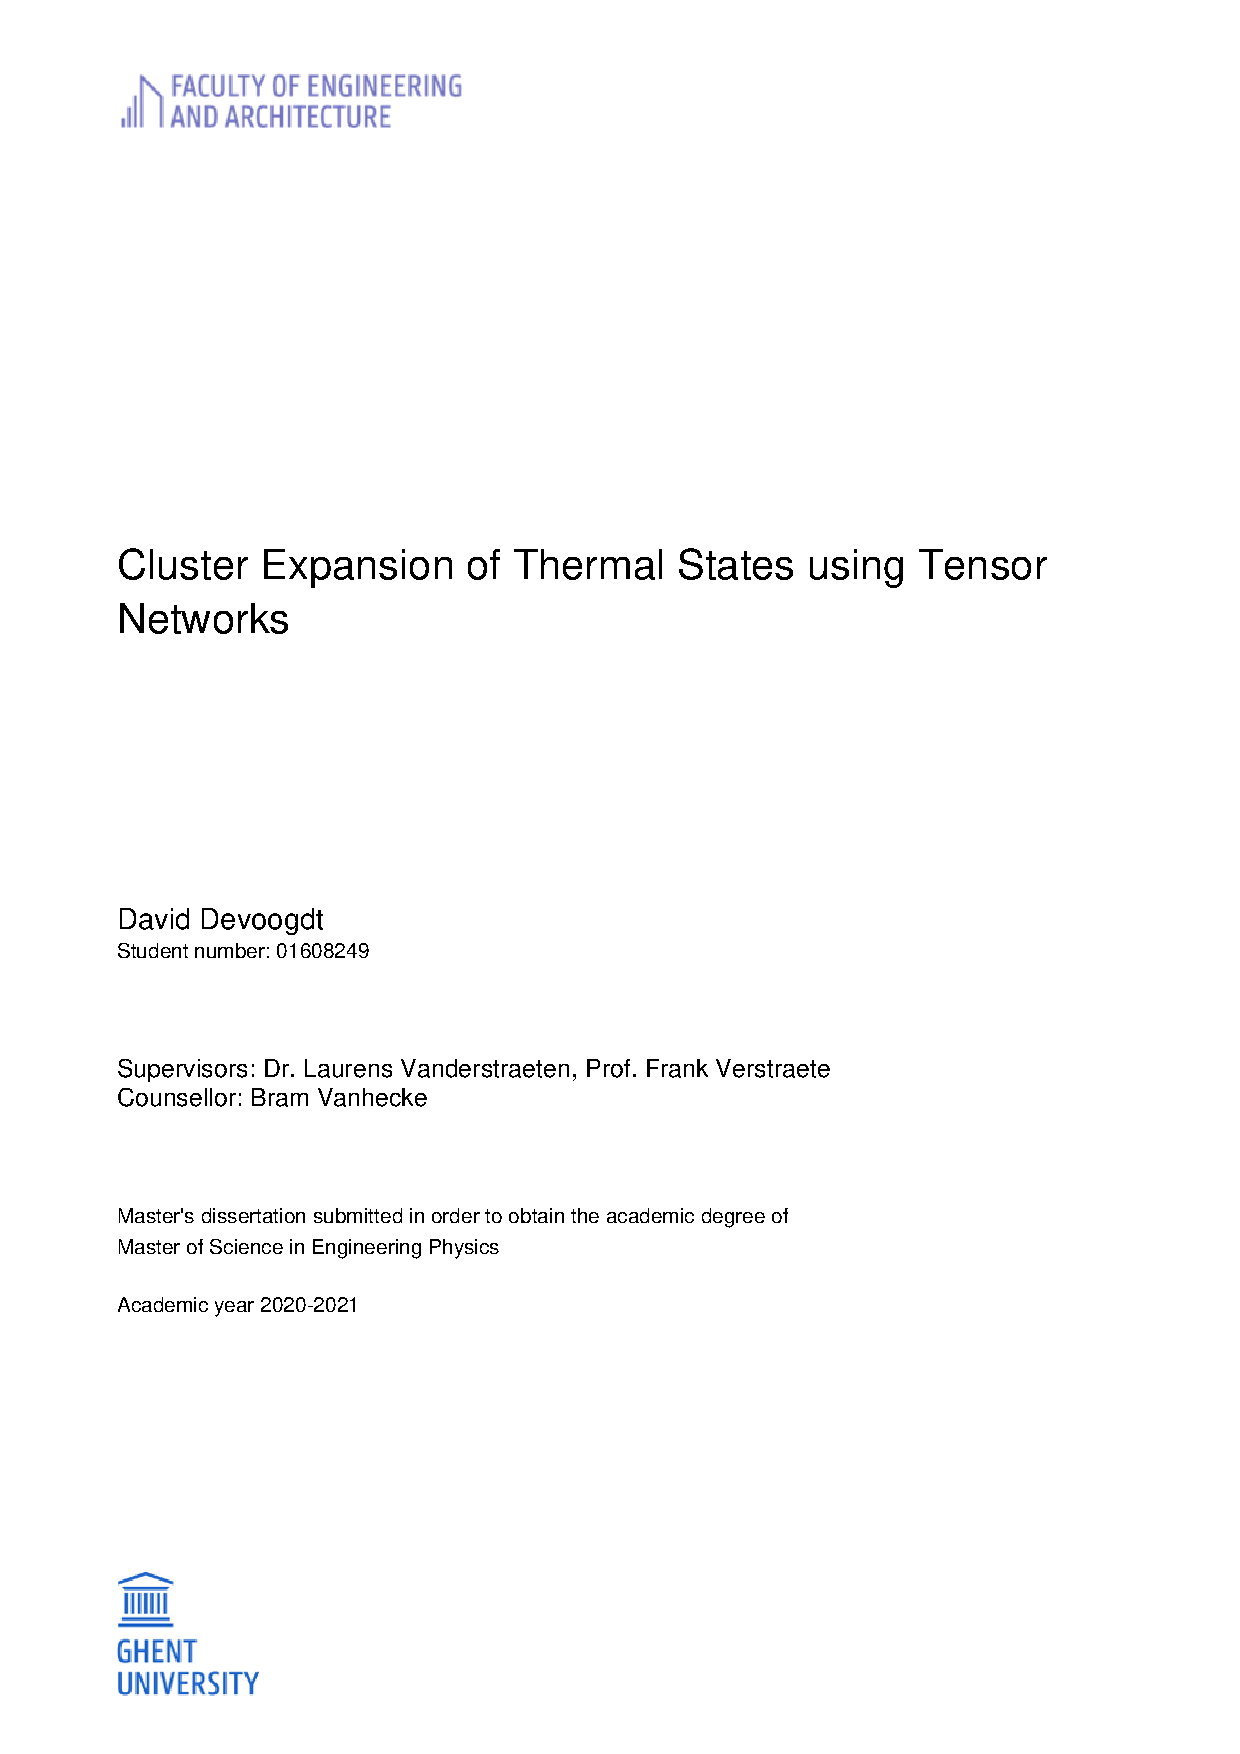
\includepdf[pages={1}]{ titelblad.pdf }

\newpage
\thispagestyle{empty}
\mbox{}
\newpage

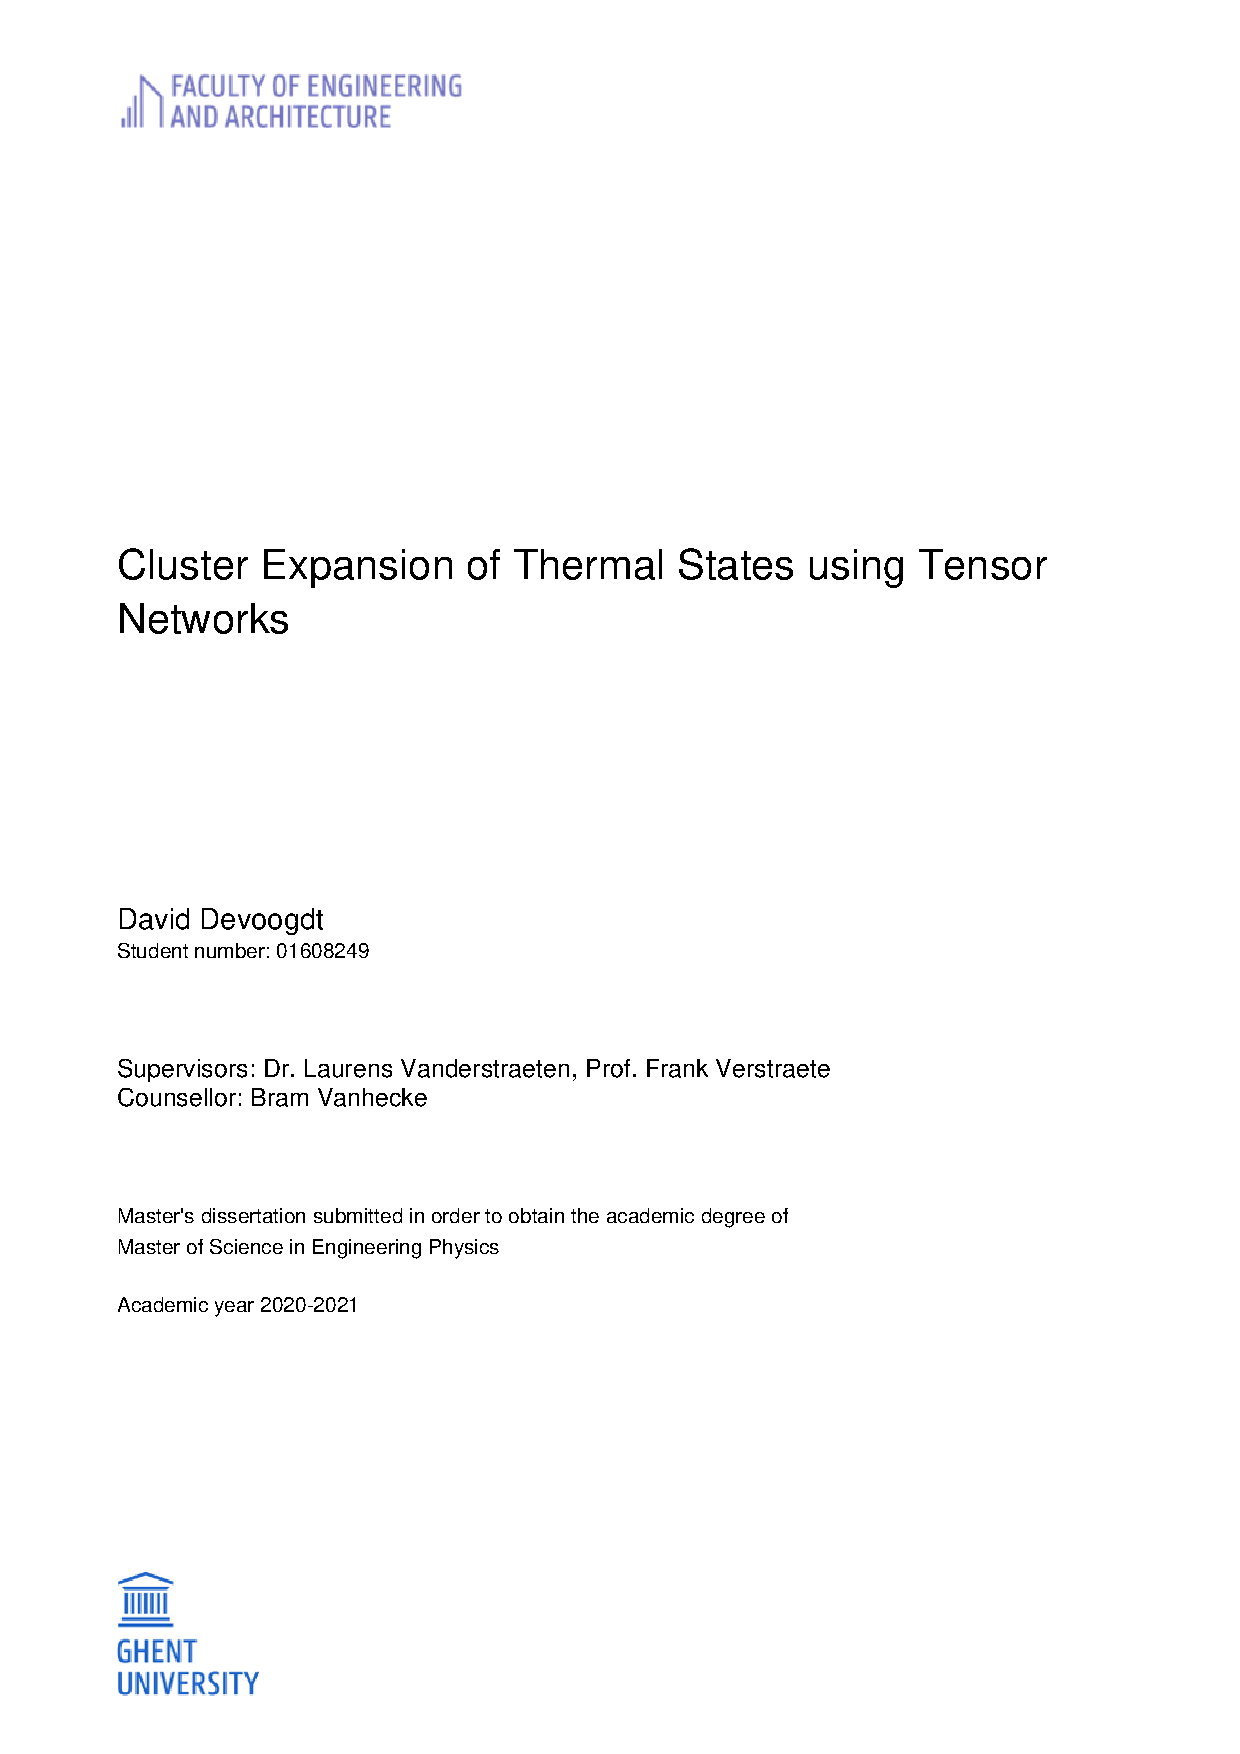
\includepdf[pages={1}]{ titelblad.pdf }

\newpage

\addcontentsline{toc}{chapter}{Foreword}
\section*{Foreword}
During the preliminary first meeting, the quantum group promised me if I'd do a master's thesis in there, I'd get a challenging subject tailored to my interests. I can say that this has absolutely been the case. The quantum group gave me a taste of real research, and introduced me to many exciting (and for someone with an engineering background sometimes unknown) topics during the Friday "lunch talks".
While this is an individual task, I certainly was not on my own. Firstly I want to thank my supervisors Laurens Vanderstraeten, Frank Verstraete and my counsellor Bram Vanhecke for the interesting discussions and feedback given during the year.
I also want to thank my friends and fellow students with who I spend many memorable nights in Ghent. They made my students years truly unforgettable. Also BEST Ghent deserves a mention, because despite the Covid-19 pandemic, my board year is something I won't forget. But most importantly, I want to thank my parents for giving me the chance to study in the first place.

David Devoogdt
Ghent, 29\textsuperscript{th} May 2021


\newpage
\section*{Permission of use on loan}

\vspace*{\fill}

The author(s) gives (give) permission to make this master dissertation available for consultation and to copy parts of this master dissertation for personal use. In all cases of other use, the copyright terms have to be respected, in particular with regard to the obligation to state explicitly the source when quoting results from this master dissertation.

David Devoogdt, May 2021

\newpage

\addcontentsline{toc}{chapter}{Abstract}

\begin{center}

  \Large{\textsc{Cluster Expansion of Thermal States using Tensor
      Networks}} \\  [0.2cm]

  David Devoogdt \footnote{Student number: 01608249 }\\ [0.3cm]

  \normalsize{Supervisors: Dr. Laurens Vanderstraeten, Prof. Frank Verstraete} \\
  \normalsize{Counsellors: Bram Vanhecke} \\ [0.2cm]
  Faculty of Engineering and Architecture Ghent University\\[0.2cm]
  \small{Master's dissertation submitted in order to obtain the academic degree of \\
    Master of Science in Engineering Physics} \\ [0.2cm]
  \normalsize{Academic year 2020-2021} \\

\end{center}

\section*{Abstract}

There is a theory which states that if ever anyone discovers exactly what the Universe is for and why it is here, it will instantly disappear and be replaced by something even more bizarre and inexplicable.
There is another theory which states that this has already happened.

\section*{Keywords}

Tensor networks, Thermal States, Cluster Expansions, Phase transitions, Transverse Field Ising model

\newpage

\addcontentsline{toc}{chapter}{Extended abstract}

\includepdf[pages={1-},pagecommand={\thispagestyle{plain}}]{ extended_abstract/Extended_abstract.pdf }

\setcounter{tocdepth}{3}
\tableofcontents

\newpage

\addcontentsline{toc}{chapter}{Glossaries}

\printglossary[type=\acronymtype,nonumberlist,nogroupskip]

% \newglossaryentry{MPS}
% {
%     name=MPS,
%     description={Matrix Product State}
% }

% \newglossaryentry{MPO}
% {
%     name=MPO,
%     description={Matrix Product Operator}
% }

% \listoffigures

\mainmatter

%H1

\chapter{Introduction}\label{chap1}

\epigraph{There is nothing new to be discovered in physics now. All that remains is more and more precise measurement.}{Lord Kelvin, 1900}


\section{Introduction}

In 2015, there were about 5.6 million known physics papers in literature. At the current rate, this number doubles every 18.7 years \cite{Sinatra2015}. Despite this enormous body of literature, there are a lot of things which are not completely understood. Some examples include a self-consistent theory of quantum gravity, the need for dark energy and matter in cosmology, the arrow of time, the matter-antimatter asymmetry. There even is no interpretation of quantum mechanics where everyone agrees upon \cite{Lulea2015}.
But certainly not all open problems have to do with 'new' physics. In many areas of physics, computing the implications of relatively simple laws becomes exceedingly difficult for many particles. Of historical importance is the classical three-body problem, describing the trajectory of 3 gravitational bodies such as the earth, moon and sun. The general case is not solved, despite developments over the last 300 years \cite{Musielak2014}.
In reality, the real challenge is to model the macroscopic properties of quantum many-body system with around $10^{23}$ particles. This broad field is called condensed matter physics and is important across many disciplines, including physics, chemistry, biology, engineering. Its practitioners include those who discover and develop new materials, those who seek to understand such materials at a fundamental level through experiments and theoretical analysis, and those who apply the materials to create new devices and technologies.  \cite{Mora-Aznar2000}
In computational chemistry, the many-body problem is tackled with methods which fall in one of the following categories: ab-initio methods, density functional theory (DFT), (semi-)empirical methods and for large scale force-field methods \cite{Lewars2011}. The ab-initio methods such as (post-) Hartree-Fock methods are successful at calculating molecule geometries, molecule energies, thermodynamic properties, etc. \cite{Lewars2011}
Still, these methods are not fully able to capture all the properties of the so-called strongly correlated matter. They are defined in \cite{Alexandradinata2020} as "a correlated electron problem is one in which interactions are so strong or have a character such that theories based on the underlying original “bare” particles fail even qualitatively to describe the material properties".
There exist different methods to investigate these exciting materials. A very limited number of models is quantum integrable, meaning they can be solved in a non pertubative way. Also, some properties of models near criticality can be determined exactly with conformal field theory (CFT). But for most systems, we can only simulate the behaviour with numerical techniques. To make progress, new fast and accurate numerical methods are needed, because exact diagonalisation becomes unfeasible for large systems. Some examples of such numerical techniques, which will not be discussed here, are: Dynamical Mean Field (DMFT) / Dynamical Cluster Approximation  (DCA), Series expansion, Density Matrix Embedding Theory (DMET), Fixed-node Monte Carlo, Diagrammatic Monte Carlo, Variational Monte Carlo, Functional renormalization group (FRG) and Coupled-cluster methods. \cite{Corboz}. In this thesis, a technique is proposed that builds on the broad field of \Glspl{TN}.
Strongly correlated electron systems host a tremendous variety of fascinating macroscopic phenomena including high-temperature superconductivity, quantum spin-liquids, fractionalized topological phases, and strange metals \cite{Alexandradinata2020}.
%http://benasque.org/2020scs/talks_contr/106_tensornetworks_lecture1.pdf

\section{Tensor networks}

One problem that makes simulation of large quant systems difficult is the exponentially large size of the Hilbert space.  This is often referred to as the curse of dimensionality. But it turns out that Hilbert space of a many-body quantum system is far too large: all physical states, that is, all states that can ever be created, live on a tiny submanifold of measure zero \cite{Cirac}. More precisely, the physical states obey the so called 'area law', which states that the entanglement of a system scales according to its area and not the volume. Tensor Networks automatically have this property, making them an efficient description of a quantum system.

%https://arxiv.org/pdf/2011.12127.pdf

\section{Outline thesis}

This master's thesis is organised as follows. \Cref{chap2} gives a practical introduction to Tensor Networks. Some important TN algorithms are discussed, including the VUMPS algorithm to contract infinite lattices. \Cref{chap3} treats phases of matter and criticality and some selected quantum models. The importance of operator exponentials is explained. \Cref{chap4} introduces the central topic of this thesis: TN cluster expansion to simulate operator exponentials. \Cref{chap5} treats the implementation aspects of the cluster expansions, in particular the numerical solvers. \Cref{chap:results} measures the accuracy of the cluster expansion in 1D and 2D. Also, some the phase transitions 2D \Gls{TFI} model are calculated and compared with results from literature.

\chapter{Tensor networks}\label{chap2}

\epigraph{We could, of course, use any notation we want; do not laugh at notations; invent them, they are powerful. In fact, mathematics is, to a large extent, invention of better notations.}{Richard Feynman}

\section{Introduction}
\Glspl{TN} form a vast subject. This chapter gives a very brief introduction into the field of \Glspl{TN}. First, the graphical notation used to represent these tensors is explained. The most relevant kinds of \Glspl{TN} for this dissertation are introduced. A practical introduction is given how to manipulate these networks. Next, a selected number of \gls{MPS} algorithms are given. The focus will be to understand the intuition behind them, but not to  provide a mathematical rigorous treatment. The next section treats the contraction of infinite dimensional 2D networks. This is chosen both to improve the understanding of \Glspl{TN} through example, and because one of the algorithms, \gls{VUMPS}, will be widely used in to calculate 2D phase transition later on.

\section{Tensor networks}

\subsection{Graphical notation}

Before explaing tensor networks, some graphical notation should be introduced. This really is a way to conveniently write vectors, matrices an in general tensors without the need to introduce many labels. A tensor T is represented by a circle with a number of external legs, according to the number of external indices. Connected legs are summed. Some examples are shown in \cref{tab:grafical_not}. Every leg which is connected to multiple tensors, is contracted.

\begin{table}[]
    \centering
    \caption{Caption}
    \begin{tabular}{l|l|l}
        conventional            & Einstein                & tensor notation           \\
        \hline
        $\Vec{x}$               & $x_{\alpha}$            &

        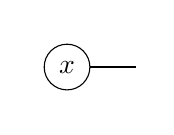
\begin{tikzpicture}[baseline=({N2.base}) ]
            \clip (-0.5,-0.5) rectangle (1,0.5);
            \node[circle, draw] (N2) at (0,0) {$x$};
            \node[] (N1) at (1,0) {};
            \draw  (N1) -- (N2) ;
        \end{tikzpicture}                                                     \\
        M                       & $M_{\alpha \beta}$      & 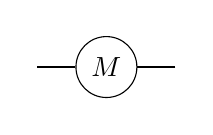
\begin{tikzpicture}[baseline={0cm-0.5*height("$=$")} ]
            \clip (-1,-0.5) rectangle (1,0.5);

            \node[circle, draw] (N2) at (0,0) {$M$};
            \node[] (N0) at (-1,0) {};
            \node[] (N1) at (1,0) {};

            \draw  (N1) -- (N2) ;
            \draw  (N0) -- (N2) ;

        \end{tikzpicture} \\

        $\Vec{x} \cdot \Vec{y}$ & $x_{\alpha} y_{\alpha}$ & 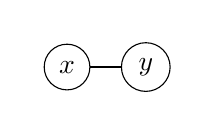
\begin{tikzpicture}[baseline=({N2.base}) ]
            \clip (-0.5,-0.5) rectangle (1.5,0.5);
            \node[circle, draw] (N2) at (0,0) {$x$};
            \node[circle, draw] (N1) at (1,0) {$y$};
            \draw  (N1) -- (N2) ;
        \end{tikzpicture} \\
    \end{tabular}

    \label{tab:grafical_not}
\end{table}

\subsection{Representing a quantum state}

Tensor network come in many shapes and forms. Tensor networks are really used to represent a tensor with many legs. A general quantum state with N sites can be described in a given basis $\ket{i}$ in the following way:
\begin{equation}
    \ket{\Psi} = \sum_{i_1 i_2 \cdots i_n } C^{i_1 i_2 \cdots i_n} \ket{i_1} \otimes \ket{i_2} \otimes \cdots \otimes \ket{i_n}
\end{equation}
Here the tensor $C$ holds all the information of the quantum state. The graphical representation can be seen in \cref{fig:tens:intro:C}.
\begin{figure}
    \centering

    \begin{tikzpicture}[ ]

        \draw (-3,-0) rectangle (1,1)  [add reference=C]   ;
        \node  at (C center) {C};

        \node (N1)  at  (-2.5,-1) {};
        \node (N2)  at  (-1.5,-1) {};
        \node  at  (-.5,-0.5) {...};
        \node  (N3) at  (.5,-1) {};

        \draw    (N1) -- (N1 |-  C south);
        \draw    (N2) -- (N2 |-  C south);
        \draw    (N3) -- (N3 |-  C south);

    \end{tikzpicture}

    \caption{Caption}
    \label{fig:tens:intro:C}
\end{figure}

This requires an exponential number $d^n$ of coefficients C where d is the dimensions of basis $\ket{i}$. In order to make the problem tractable, the following form is proposed as wave function:
\begin{equation}
    C^{i_1 i_2 \cdots i_n} = {C^{1}}_{\alpha_1}^{ i_1} {C^{2}}_{\alpha_1 \alpha_2}^{i_2} \cdots  {C^{n}}_{\alpha_{n-1} }^{i_n}
\end{equation}

\begin{equation}
    \mpo{4}{{"-",,,,,}}{{"$i_1$","$i_2$",,"$i_n$","-"}}{{"-","-",,"-","-"}}{{0,0,1,0,0}}{{"$C^1$", "$C^2$",,"$C^n$", }}
\end{equation}

Where summation over shared indices is implied. It is always possible to find such a representation by means of matrix decomposition (see \cref{sec:mpomath}). The summation over $\alpha_i$ are called a virtual bond and their dimension is denoted by $\chi$. At this point, this is not yet an improvement because the bond dimension needs to be exponentially large in order to represent the tensor C exactly.

Explicit translational invariance is given by tensor $C^i_{\alpha \beta }$ that don't depend on the location. The chain is closed by a matrix M which contains the boundary condiditions. Setting $\alpha_n = \alpha_0$. We can now write this as a Trace over matrix products:

\begin{equation}
    \ket{\Psi} = \Tr( C^{i_1} C^{i_2} \cdots C^{i_n} M  ) \ket{i_1} \otimes \ket{i_2} \otimes \cdots \otimes \ket{i_n}
\end{equation}

\begin{equation}\label{eq:general_mps}
    \mpo{5}{{"Tr",,,,,}}{{"$i_1$","$i_2$",,"$i_n$","-"}}{{"-","-",,"-","-"}}{{0,0,1,0,0}}{{"C", "C",,"C","M" }}
\end{equation}

\subsection{Classification}

Tensor networks come in many shapes and many forms. During this thesis, we will mainly encounter the types explained here.

\subsubsection{MPS}

A general MPS is of the form \cref{eq:general_mps}. For an infinite extended chain with translation invariance, it is logical to assume an unit cell:
\begin{equation}\label{mps:uni}
    \pepob{5}{2}{{
                "-","-", "-","-",
                "","","",""}}{{
                "-",
                "",
                "",
                "",
                "-"}}{{
                4,4,4,4,4,
                13,0,0,0,13}}
\end{equation}
This will be the form we will work with in this thesis. Of course, larger unit cells are also possible.

MPS are dense. This means that (with a bond dimension exponential in the system size) the MPS can represent every state in the full Hilbert space.  \cite{Orus2014}. However, the low energy states can typically be represented by a much lower bond dimension.

This can be explain in terms of the so called 'area law': the entropy low energy states often scale with the boundary area of volume. MPS exactly follow this area law.

\subsubsection{MPO}

Similarly to an MPS, a Matrix Product Operator (MPO) is of the following form:

\begin{equation} \label{def_mpo}
    \begin{split}
        \hat{O} &= \sum Tr(A^{i_1 j_1} A^{i_2 j_2} \cdots A^{i_n j_n} M) \\
        & \times \ket{i_1}\bra{j_1} \otimes \ket{i_2}\bra{j_2} \otimes \cdots \otimes \ket{i_n}\bra{j_n} \\
        &\mpo{5}{{"Tr",,,,,}}{{"$i_1$","$i_2$",,"$i_n$","-"}}{{"$j_1$","$j_2$",,"$j_n$","-"}}{{0,0,1,0,0}}{{"A", "A",,"A","M" }}
    \end{split}
\end{equation}

The matrix M contains the boundary conditions of the operator. Its clear that this can again be made translation invariant. Acting with an MPS on a MPO $\hat{O} \ket{\Psi} $ again results in a MPS, as expected.

An uniform MPO is denoted by:
\begin{equation}
    \pepob{5}{3}{{
                "-","-", "-","-",
                "","","","",
                "-","-", "-","-",}}{{
                "-","-",
                "","",
                "","",
                "","",
                "-","-",}}{{
                4,4,4,4,4,
                13,0,0,0,13,
                4,4,4,4,4,}}
\end{equation}

This can also be reinterpreted as an MPS with physical bond dimension $D^2$, by grouping the i and j indices together per site.

\paragraph{Examples of MPO hamiltonians} \cref{mpo_hamil}

\subsubsection{PEPS}
Projected entangled pair states (PEPS) are the 2D equivalent of MPS. In the visualisation, the physical indices come out of the plane.
\begin{equation}
    \vcenter{ \hbox{ \pepob{5}{5}{{
                        "-","-", "-","-",
                        "",  "", "","",
                        "",  "", "","",
                        "",  "", "","",
                        "-", "-", "-","-",}}{{
                        "-","-", "-","-",
                        "","", "","",
                        "","", "","",
                        "","", "","",
                        "-","-", "-","-",}}{{
                        1,13,13,13,1,
                        13,15,15,15,13,
                        13,15,15,15,13,
                        13,15,15,15,13,
                        1,13,13,13,1,
                    }} }}
\end{equation}

\subsubsection{PEPO}

The operator version of PEPS is called PEPO. The depiction looks as follows:
\begin{equation}
    \vcenter{ \hbox{ \pepob{5}{5}{{
                        "-","-", "-","-",
                        "",  "", "","",
                        "",  "", "","",
                        "",  "", "","",
                        "-", "-", "-","-",}}{{
                        "-","-", "-","-",
                        "","", "","",
                        "","", "","",
                        "","", "","",
                        "-","-", "-","-",}}{{
                        1,13,13,13,1,
                        13,14,14,14,13,
                        13,14,14,14,13,
                        13,14,14,14,13,
                        1,13,13,13,1,
                    }} }}
\end{equation}

\subsubsection{Others}

To show there exist many more tensor network beside the ones treated in this thesis, 2 examples are shown in \cref{fig:tnalgs:ttn_mera}.

Two Tree tensor networks (TTNs)  are shown. The red indices are physical. MERA (c) is also shown. These tensor network are specific because they can be contracted exactly, as opposed to for instance PEPS.

\begin{figure}
    \center
    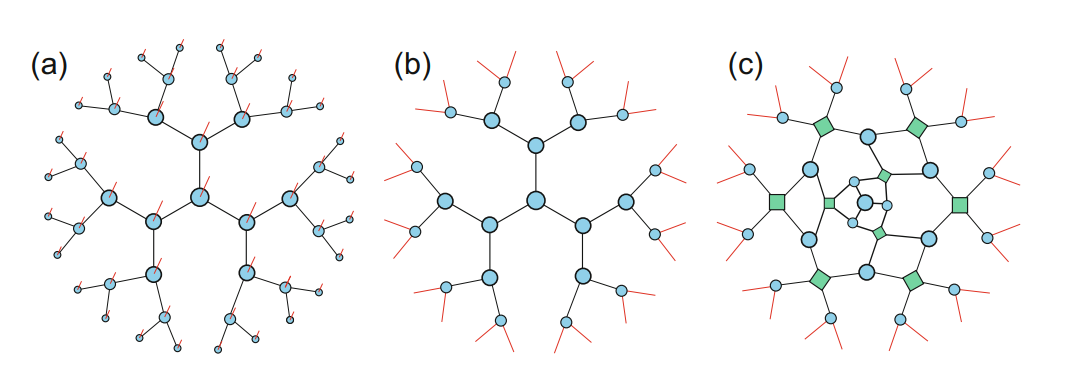
\includegraphics[width=0.8 \textwidth]{Figuren/tnalgs/tnns_and_mera.png}
    \caption{ (a) and (b) two different TTNSs and (c) MERA. Figure taken from \cite{Ran2020}.  }
    \label{fig:tnalgs:ttn_mera}
\end{figure}

%https://link.springer.com/content/pdf/10.1007%2F978-3-030-34489-4.pdf

\section{TN manipulations}\label{sec:mpomath}
This section serves as an introduction of tensor network manipulations. The overview mainly focusses on MPS/MPO networks, but most of the operations translate to the 2D case.

The MPS's are processed by transforming the tensor into a matrix, performing some matrix calculations and casting it back into its original form. In this way, the standard methods from linear algebra can be used. This section gives some examples how this is done in practice:

\subsection{Basics}

\subsubsection{Grouping legs}
One of the most basic manipulations is to group some legs of a tensor into one leg:
\begin{equation}
    \begin{split}
        T^{i_1 i_2 j_1 j_2} &=  \expH{2}{$T$}{{"$i_1$","$i_2$"}}{{"$j_1$","$j_1$"}}{} \\
        & \cong \expH{2}{$T$}{{"-","-"}}{{"-","-"}}{{"$(i_1 j_1 )$","$(i_2 j_2)$"}} \\
        &= T^{ (i_1 j_1 ) (i_2 j_2) } \\
    \end{split}
\end{equation}
The dimension of the new leg is the product of the dimension of the individual legs. Contracting 2 merged legs with 2 merged legs is exactly the same as contracting them separately. The 4 leg tensor and matrix contain exactly the same information.
Manipulating this in memory requires both permute and reshape commands. This requires some time as the internal representation of the matrix changes.

\subsubsection{Decomposition} \label{decompMPO}

The grouping above can be applied to decompose a tensor into 2 tensors with matrix techniques. An example, which will be needed later on, is give here.

\def \figone {\expH{2}{$O^{u v,v w}$}{{"$i_1$","$i_2$"}}{{"$j_1$","$j_1$"}}{{"u","w"}}}

\begin{equation}
    \begin{split}
        \figone &= O^{i_1 i_2 j_1 j_2 }_{\alpha_u \gamma_w} \\
        &\cong O^{u w}_{ (\alpha_u i_1 j_1) (\gamma_w i_2 j_2) } \\
        &= O^{u v}_{(\alpha_u i_1 j_1) \alpha_v } O^{v w}_{ \alpha_v (\alpha_w i_2 j_2) } \\
        &\cong \mpo{2}{{"u","v","w"}}{{"$i_1$","$i_2$"}}{{"$j_1$","$j_1$"}}{}{}
    \end{split}
\end{equation}

The indices U, V and W represent block indices. Step 2 reshapes and groups the indices on to one index on the left and one on the right. The dimension of this index is the product of the separate dimensions. Step 3 decomposes the matrix into a product of 2 matrices. The last step transforms the indices back to separate legs.

For an exact representation, the bond dimension of virtual level v is the product of the dimensions of the outer legs
\begin{equation}
    \dim{v} = \min( \dim{u}, \dim{v}) \cdot ( \dim{i}  ) ^2 .
\end{equation}

Many matrix decompositions exist. Some useful examples here are SVD decomposition, eigenvalue decomposition, QR, $\cdots$.

\subsubsection{Truncation}

The above procedure also gives a way to truncate the bond dimension: first take together 2 neighbouring sites, then perform an SVD $T = U \Sigma V^{\dagger}$. Split as follows:
\begin{equation}
    T = \begin{bmatrix}
        U_1 & U_2 \\
    \end{bmatrix} \begin{bmatrix}
        \Sigma_1 & 0        \\
        0        & \Sigma_2 \\
    \end{bmatrix} \begin{bmatrix}
        V_1 & V_2\\\end{bmatrix}^{\dagger}
\end{equation}
where $\Sigma_1$ contains the n largest singular values. Then $\hat{T} = U_1 \Sigma_1 V_1^{\dagger}$ is the best rank n approximation to the original tensor.
\begin{equation}
    min_{rank(A) \leq n } \| T-A  \|  = \| T- \hat{T}  \|
\end{equation}

\subsubsection{Virtual levels}
In the previous example, the levels were indicated with a block index or virtual level. The idea is to separate the contraction into blocks. This is completely analogous to matrix block multiplication. This will be a more natural form to represent the algorithm. Of course, one can easily switch between block representation and the full one.

\subsubsection{Inversion}
Suppose we want to find a MPO O for given tensors A and B such that the following holds:

\def \figone {\expH{2}{$A$}{{"$i_1$","$i_2$"}}{{"$j_1$","$j_2$"}}{{"u",}}}
\def \figthree {\expH{3}{$B$}{{"$i_1$","$i_2$","$i_3$"}}{{"$j_1$","$j_2$","$j_3$"}}{{"u","v"}}}

\def \figtwo {\mpo{1}{{,"v"}}{{"$i_3$",}}{{"$j_3$",}}{}{}}

\begin{equation}
    \combineTikz{ \figone }{\figtwo}{1.8} =  \figthree
\end{equation}

Again, the indices can be taken together in the following way: $\alpha = (u i_1 j_1  i_2 j_2)$ and $\beta = (i_3 j_3 v)$:
\begin{equation}
    A_{\alpha \gamma} O_{\gamma \beta} = B_{\alpha \beta}
\end{equation}
This is a standard matrix equation and can hence be solved with linear algebra packages. Note that it is not necessary to calculate $A^{-1}$ to obtain the solution, linear solver are generally much faster. As this is one of the core problems to solve both in 1D and 2D, this will be discussed in detail in \cref{sec:framework_impl}.

\subsubsection{Contraction order}

Tensor network diagram determine unambiguously the result of a contraction. This does not mean all contraction orders are equivalent. The number of operations needed to contract 2 vectors is D. Each additional leg multiplies the number of operations by the bond dimension. Two different contraction orders are shown in \cref{fig:tnalgs:cont_ord}.

\begin{figure}[H]
    \center
    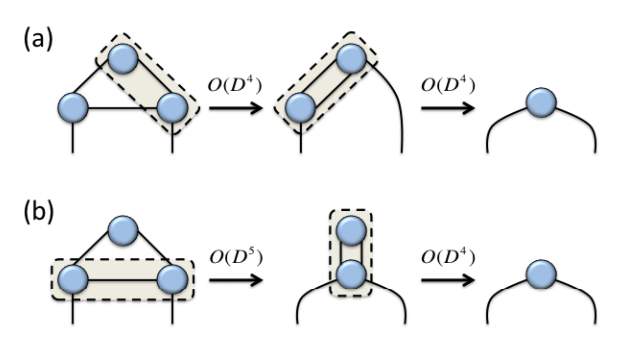
\includegraphics[width=0.8 \textwidth]{Figuren/tnalgs/contraction_order.png}
    \caption{ (a) Contraction of 3 tensors in $O(D^4)$ time (b) Contraction of same tensors in $O(D^5)$ time. Figure taken from \cite{Orus2014}.  }
    \label{fig:tnalgs:cont_ord}
\end{figure}

%\section{\Gls{TN} algorithms}

\section{MPS algorithms}

This section and the following one, will introduce some different tensor network algorithms. The gaol is to provide an intuitive explanation how these algorithms work. For rigorous derivations and mathematical details, other sources can be read.

\subsection{Canonical form}

A translation invariant MPS has the following form shown in \cref{mps:uni}

It can be easily seen that inserting $X X^{-1}$ on each bond doesn't change the contracted tensor. This is called a gauge transformation.
\begin{equation}
    A_l = \pepob{3}{2}{{
                "-","-",
                "",""}}{{
                "-",
                "",
                "-"}}{{
                4,4,4,
                4,2,4}}  =X \pepob{3}{2}{{
                "-","-",
                "",""}}{{
                "-",
                "",
                "-"}}{{
                4,4,4,
                4,0,4}} X^{-1}
\end{equation}

\begin{equation}
    A_r = \pepob{3}{2}{{
                "-","-",
                "",""}}{{
                "-",
                "",
                "-"}}{{
                4,4,4,
                4,3,4}}=Y \pepob{3}{2}{{
                "-","-",
                "",""}}{{
                "-",
                "",
                "-"}}{{
                4,4,4,
                4,0,4}} Y^{-1}
\end{equation}
and
\begin{equation}
    \pepob{3}{2}{{
                "-","-",
                "",""}}{{
                "-",
                "-",
                "-"}}{{
                4,4,4,
                4,6,4}}  = X Y^{-1} = C
\end{equation}
Then \cref{mps:uni}  can be written as follows:
\begin{equation}
    \pepob{6}{2}{{
                "-","-", "-","-","-",
                "","","","",""}}{{
                "-",
                "",
                "",
                "-",
                "",
                "-"}}{{
                4,4,4,4,4,4,
                4,2,2,6,3,4}}
\end{equation}
Introducing one more tensor:
\begin{equation}\label{algs:ACC}
    A_c = \pepob{3}{2}{{
                "-","-",
                "",""}}{{
                "-",
                "",
                "-"}}{{
                4,4,4,
                4,7,4}} = \pepob{4}{2}{{
                "-","-", "-",
                "","",""}}{{
                "-",
                "",
                "-",
                "-"}}{{
                4,4,4,4,
                4,2,6,4}} = \pepob{4}{2}{{
                "-","-", "-",
                "","",""}}{{
                "-",
                "-",
                "",
                "-"}}{{
                4,4,4,4,
                4,6,3,4}}
\end{equation}
At the moment the matrices $X$ and $Y$ are not yet defined. To bring an MPS A in its canonical form, the following choice is made:

\begin{subequations} \label{algs:mpsid}
    \begin{alignat}{3}
                     & \vcenter{ \hbox{ \pepob{3}{2}{{
                            "","",
                            "",""}}{{
                            "",
                            "",
                            "-"}}{{
                            4,2,4,
        4,2,4}} } }= &                                 & \vcenter{ \hbox{  \pepob{3}{2}{{
                            "","-",
                            "","-"}}{{
                            "",
                            "-",
                            "-"}}{{
                            4,4,4,
        4,4,4}} } }  &                                 & = I                              \\
                     & \vcenter{ \hbox{ \pepob{3}{2}{{
                            "","",
                            "",""}}{{
                            "-",
                            "",
                            ""}}{{
                            4,3,4,
        4,3,4}} } }= &                                 & \vcenter{ \hbox{  \pepob{3}{2}{{
                            "","-",
                            "","-"}}{{
                            "",
                            "-",
                            "-"}}{{
                            4,4,4,
        4,4,4}} } }  &                                 & = I
    \end{alignat}
\end{subequations}

The tensors below are the conjugated version of the tensors above. There is still some freedom: a unitary gauge transformation can still be applied. With this choice, it is possible to bring $C$ in diagonal form.

\subsubsection{Entropy}

The canonical form above is very convenient to calculate the entropy, which is given by
\begin{equation}
    S = -\sum_i \alpha_i^2 \log (\alpha_i^2 )
\end{equation}
where $\alpha_i$ are the singular values of $C$.

\subsubsection{Expectation value}\cref{subsec:exp_val_1d}

One property of MPS is that expectation values can be calculated exactly. Suppose we have an operator $\hat{O}$ acting on a single site of the MPS: $\Braket{ \Psi |  \hat{O} | \Psi  }$
\begin{equation}
    \vcenter{\hbox{\pepob{5}{3}{{
                        "","", "","",
                        "-","-","-","-",
                        "","","","",}}{{
                        "-", "-",
                        "", "",
                        "", "",
                        "", "",
                        "-", "-",}}{{
                        13,2,7,3,13,
                        1,4,0,4,1,
                        13,2,7,3,13}} }}  =   \vcenter{\hbox{\pepob{5}{3}{{
                        "","", "","",
                        "-","-","-","-",
                        "","","","",}}{{
                        "-", "*-",
                        "", "",
                        "", "",
                        "", "",
                        "-", "-",}}{{
                        1,4,7,4,1,
                        1,4,0,4,1,
                        1,4,7,4,1}} }}
\end{equation}
where we made use of \cref{algs:mpsid}. Similar techniques allow calculating correlation functions, energies, ...

\section{Tensor network contraction}

The contraction in this section is somewhat different. The MPO with the same $S_n =  (i_1 i_2 \cdots i_n) = (j_1 j_2 \cdots j_n)$ represents the probability of finding the system in state $S_n$.  This will be needed in \cref{subsec:statmech}. On a patch, an operator X is applied. This could be a measurement.

\subsection{1D problem}

Suppose that the there is an MPO representation A that gives the probability of a state, and an operator X which performs a measurement over a number of sites. The expectation value $ \Braket{X}$ is given by:
\begin{equation}
    \Braket{X} = \frac{
        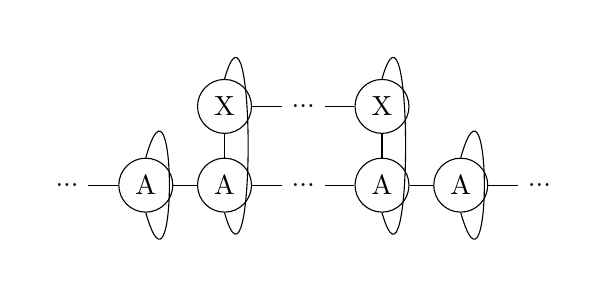
\begin{tikzpicture} [   ]
            \clip (-1.5,-1) rectangle (5.5,2);

            \node[] (N0) at (-1,0) {...};
            \node[circle, draw] (N1) at (0,0) {A};
            \node[circle, draw] (N2) at (1,0) {A};
            \node[circle, draw] (X2) at (1,1) {X};

            \node[] (N3) at (2 ,0) {...};
            \node[] (X3) at (2,1) {...};

            \node[circle, draw] (N4) at (3 ,0) {A};
            \node[circle, draw] (X4) at (3,1) {X};

            \node[circle, draw] (N5) at (4 ,0) {A};
            \node[] (N6) at (5 ,0) {...};

            \draw  (N0) -- (N1) ;

            \draw  (N1) -- (N2) ;
            \draw  (N2) -- (N3) ;
            \draw  (N3) -- (N4) ;
            \draw  (N4) -- (N5) ;
            \draw  (N5) -- (N6) ;

            \draw  (X2) -- (X3) ;
            \draw  (X3) -- (X4) ;

            \draw  (N2) -- (X2) ;
            \draw  (N4) -- (X4) ;

            \draw (X2.north)   .. controls +(0.4,1.4) and +(0.4,-1.4) .. (N2.south);
            \draw (X4.north)   .. controls +(0.4,1.4) and +(0.4,-1.4) .. (N4.south);

            \draw (N1.north)   .. controls +(0.4,1.4) and +(0.4,-1.4) .. (N1.south);
            \draw (N5.north)   ..  controls +(0.4,1.4) and +(0.4,-1.4)  .. (N5.south);
        \end{tikzpicture}
    }{
        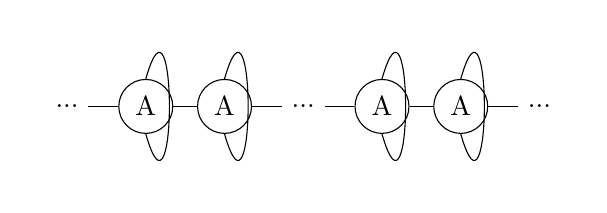
\begin{tikzpicture} [   ]

            \clip  (-1.5,-3) rectangle (5.5,-1);

            \node[] (O0) at (-1,-2) {...};
            \node[circle, draw] (O1) at (0,-2) {A};
            \node[circle, draw] (O2) at (1,-2) {A};

            \node[] (O3) at (2 ,-2) {...};
            \node[circle, draw] (O4) at (3 ,-2) {A};

            \node[circle, draw] (O5) at (4 ,-2) {A};
            \node[] (O6) at (5 ,-2) {...};

            \draw  (O0) -- (O1) ;

            \draw  (O1) -- (O2) ;
            \draw  (O2) -- (O3) ;
            \draw  (O3) -- (O4) ;
            \draw  (O4) -- (O5) ;
            \draw  (O5) -- (O6) ;

            \draw (O2.north)   .. controls +(0.4,1.4) and +(0.4,-1.4) .. (O2.south);
            \draw (O4.north)   .. controls +(0.4,1.4) and +(0.4,-1.4) .. (O4.south);

            \draw (O1.north)   .. controls +(0.4,1.4) and +(0.4,-1.4) .. (O1.south);
            \draw (O5.north)   ..  controls +(0.4,1.4) and +(0.4,-1.4)  .. (O5.south);
        \end{tikzpicture}
    }
    \label{sm:expecatation_X}
\end{equation}

In the thermodynamic limit there are an infinity number of A to the left and the right. This can be simulated by taking the left and right fixed points of the traced MPO A corresponding to the largest eigenvector $\lambda$.

\begin{equation}\label{algs:exp}
    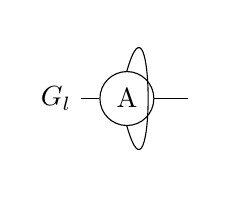
\begin{tikzpicture}[baseline={0cm-0.5*height("$=$")} , scale=0.9]
        \clip (-1.4,-1) rectangle (1,1);
        \node[] (N0) at (-1,0) {$G_l$};
        \node[] (N2) at (1,0) {};
        \node[circle, draw] (N1) at (0,0) {A};
        \draw  (N0) -- (N1) ;
        \draw  (N1) -- (N2) ;
        \draw (N1.north)   .. controls +(0.4,1.4) and +(0.4,-1.4) .. (N1.south);
    \end{tikzpicture}
    = \lambda
    \begin{tikzpicture}[baseline={0cm-0.5*height("$=$")}, scale=0.9 ]
        \clip (-.4,0.5) rectangle (1,-0.5);
        \node[] (N2) at (1,0) {};
        \node[] (N1) at (0,0) {$G_l$};
        \draw  (N1) -- (N2) ;
    \end{tikzpicture}
\end{equation}

\begin{equation}
    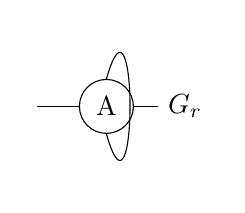
\begin{tikzpicture}[baseline={0cm-0.5*height("$=$")} ]
        \clip (-1,-1) rectangle (1.4,1);
        \node[] (N0) at (-1,0) {};
        \node[] (N2) at (1,0) {$G_r$};
        \node[circle, draw] (N1) at (0,0) {A};
        \draw  (N0) -- (N1) ;
        \draw  (N1) -- (N2) ;
        \draw (N1.north)   .. controls +(0.4,1.4) and +(0.4,-1.4) .. (N1.south);
    \end{tikzpicture}
    = \lambda
    \begin{tikzpicture}[baseline={0cm-0.5*height("$=$")} ]
        \clip (0,-0.5) rectangle (1.4,0.5);
        \node[] (N2) at (1,0) {$G_l$};
        \node[] (N1) at (0,0) {};
        \draw  (N1) -- (N2) ;
    \end{tikzpicture}
\end{equation}

Equation \cref{sm:expecatation_X} can now be easily calculated:

\begin{equation}
    \Braket{X} = \frac{
        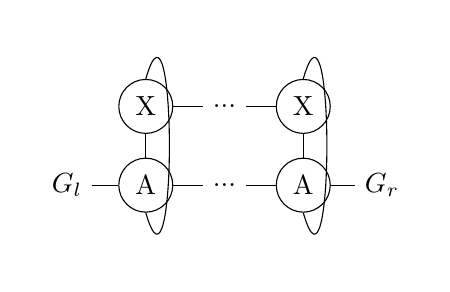
\begin{tikzpicture} [   ]
            \clip (-0.5,-1) rectangle (4.5,2);

            \node[] (N1) at (0,0) {$G_l$};
            \node[circle, draw] (N2) at (1,0) {A};
            \node[circle, draw] (X2) at (1,1) {X};

            \node[] (N3) at (2 ,0) {...};
            \node[] (X3) at (2,1) {...};

            \node[circle, draw] (N4) at (3 ,0) {A};
            \node[circle, draw] (X4) at (3,1) {X};

            \node[] (N5) at (4 ,0) {$G_r$};

            \draw  (N1) -- (N2) ;
            \draw  (N2) -- (N3) ;
            \draw  (N3) -- (N4) ;
            \draw  (N4) -- (N5) ;

            \draw  (X2) -- (X3) ;
            \draw  (X3) -- (X4) ;

            \draw  (N2) -- (X2) ;
            \draw  (N4) -- (X4) ;

            \draw (X2.north)   .. controls +(0.4,1.4) and +(0.4,-1.4) .. (N2.south);
            \draw (X4.north)   .. controls +(0.4,1.4) and +(0.4,-1.4) .. (N4.south);

        \end{tikzpicture}
    }{
        \lambda^n
        \begin{tikzpicture}[baseline={0cm-0.5*height("$=$")} ]
            \clip (-0.5,-0.5) rectangle (1.4,0.5);
            \node[] (N2) at (1,0) {$G_r$};
            \node[] (N1) at (0,0) {$G_r$};
            \draw  (N1) -- (N2) ;
        \end{tikzpicture}
    }
    \label{sm:expecatation_X_2}
\end{equation}

\subsection{2D problem}
PEPS contraction concerns a similar problem, but in 2D. Here, instead of already applying operator X, the (one site) reduced density matrix $ \rho_{i,j}$ is computed:
\begin{equation}\label{algs:biggrid}
    \rho_{i,j} =\vcenter{ \hbox{ \pepob{7}{7}{{
                        "-","-", "-","-","-","-",
                        "",  "", "","","","",
                        "",  "", "","","","",
                        "",  "", "","","","",
                        "",  "", "","","","",
                        "",  "", "","","","",
                        "-", "-", "-","-","-","-",}}{{
                        "-","-", "-","-","-","-",
                        "","", "","","","",
                        "","", "","","","",
                        "","", "","","","",
                        "","", "","","","",
                        "","", "","","","",
                        "-","-", "-","-","-","-",}}{{
                        1,13,13,13,13,13,1,
                        13,0,0,0,0,0,13,
                        13,0,0,0,0,0,13,
                        13,0,0,12,0,0,13,
                        13,0,0,0,0,0,13,
                        13,0,0,0,0,0,13,
                        1,13,13,13,13,13,1,
                    }} }}
\end{equation}
This problem is much harder than in 1D. For instance, the related problem of calculating the expectation value of on operator, similar to \cref{subsec:exp_val_1d} in 1D, is  \#P-Hard \cite{Orus2014}.

\subsection{Overview methods}

As this is a difficult task, and often the bottleneck in simulations, many algorithms exist to perform this. The classification is taken from \cite{Nietner2020}.

\subsubsection{Real-space renormalisation-group methods}

The general idea is to course grain the tensor network. Of the many methods, historically the first one was Tensor renormalisation group (TRG)  \cite{Hauru}, shown in \cref{fig:tnalgs:trg}. In the first step i, the tensor are split with an SVD in 2 different ways, depending on the position on the lattice. Step ii recombines 4 halves of the decomposition into 1 new tensor. The result is a rotated grid, with side length $\sqrt{2}$. The bond dimension is truncated during the SVD step.

\begin{figure}
    \center
    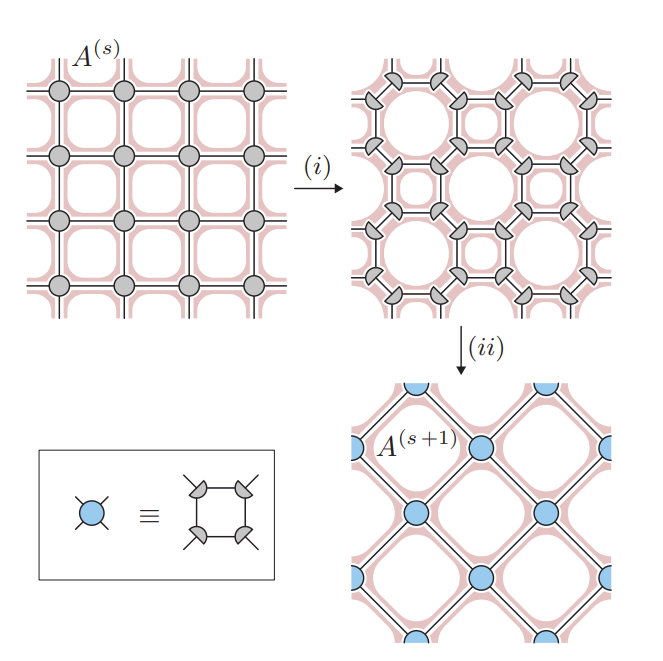
\includegraphics[width=0.8 \textwidth]{Figuren/tnalgs/TRG.png}
    \caption{ Steps in TRG procedure. Figure taken from \cite{Hauru}.  }
    \label{fig:tnalgs:trg}
\end{figure}

Many other variants exist, such as Tensor Network Renormalisation (TNR), which will not be discussed here.

\subsubsection{Corner transfer matrix  methods}

Another method goes by the name Corner transfer matrix renormalisation group (CTMRG), as described in \cite{orus}. The full network is approximated by 4 corner matrices and 4 C and 4 half row transfer matrices T as shown in \cref{fig:tnalgs:ctmrg:a}. The idea is to find matrices such that inserting a row and truncating it again results in the same tensors. This is shown in \cref{fig:tnalgs:ctmrg:b}. First, a new row is inserted. From \cref{fig:tnalgs:ctmrg:a} it can be seen that this should not change the environment. Some tensors are taken together in step 2. As a final step, the tensor are suitably truncated. Once this cycle converges, the environment is known.

\begin{figure}
    \centering
    \begin{subfigure}[b]{0.8\textwidth}
        \centering
        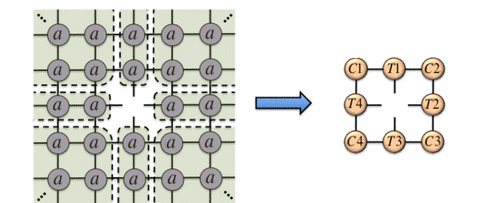
\includegraphics[width=\textwidth]{Figuren/tnalgs/CTMRG_Def.png   }
        \caption{Definition of environment}
        \label{fig:tnalgs:ctmrg:a}
    \end{subfigure}

    \begin{subfigure}[b]{0.7\textwidth}
        \centering
        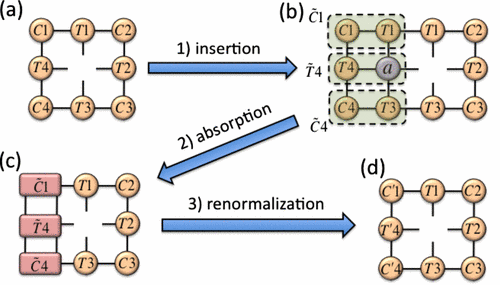
\includegraphics[width=\textwidth]{Figuren/tnalgs/CTMRG.png   }
        \caption{3 steps of CTMRG}
        \label{fig:tnalgs:ctmrg:b}
    \end{subfigure}
    \caption{  Figures adapted from \cite{orus} }
    \label{fig:tnalgs:ctmrg}
\end{figure}

Note that many important details are not written down here, and this is merely to give some intuition about tensor network contraction algorithms.

\subsubsection{Boundary methods}

The goal of these methods is to find an MPS fixed point for the infinite lattice:

\begin{equation}\label{algs:mpslayermpo}
    \pepob{5}{3}{{
                "-","-", "-","-",
                "","","","",
                "","","","",}}{{
                "-", "-",
                "", "",
                "", "",
                "", "",
                "-", "-",}}{{
                4,4,4,4,4,
                13,0,0,0,13,
                13,2,7,3,13}}  \approx  \pepob{5}{2}{{
                "-","-", "-","-",
                "","","",""}}{{
                "-",
                "",
                "",
                "",
                "-"}}{{
                4,4,4,4,4,
                13,2,7,3,13}}
\end{equation}

\paragraph{Time-evolving block decimation}

Time-evolving block decimation was introduced as a method to calculate thermal states (this will also be encountered later on in \cref{fig:tnalgs:tebd}). It can also be used as a power method for contraction.
The idea is shown in \cref{fig:tnalgs:tebd}. The boundary MPS is applied, and afterwards truncated. When this procedure is applied enough times, a fixed point is reached.

\begin{figure}
    \center
    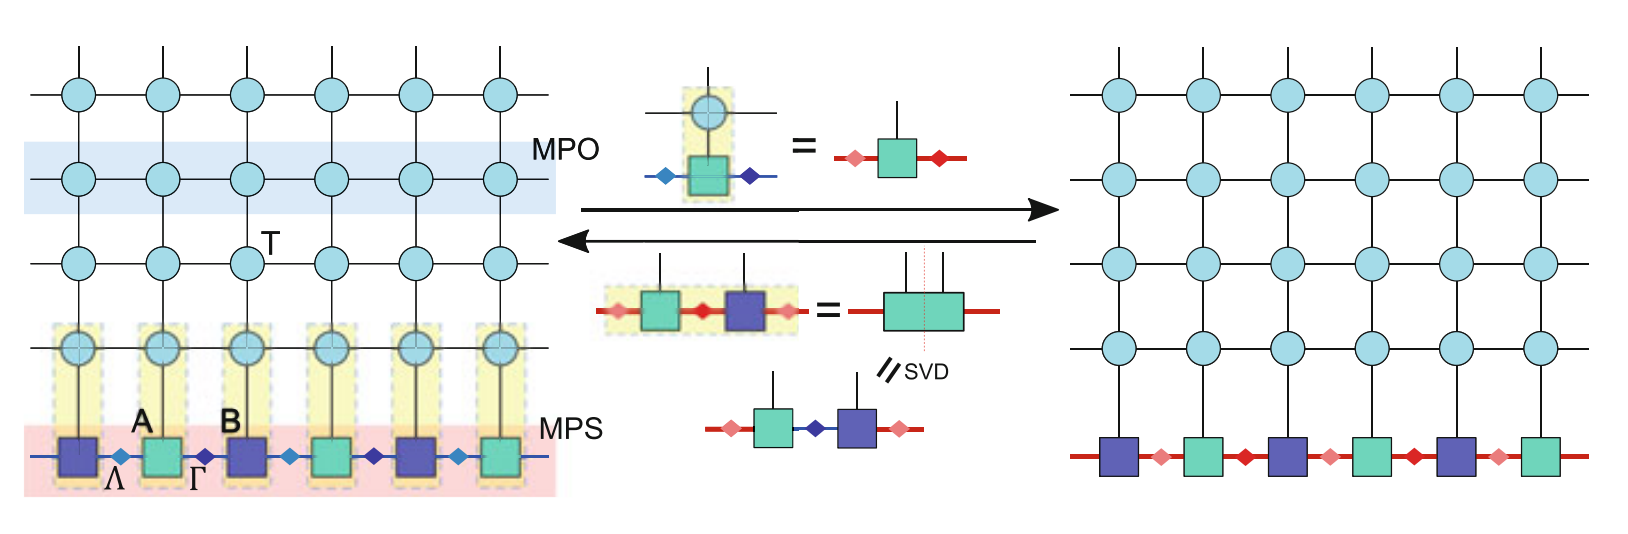
\includegraphics[width=1 \textwidth]{Figuren/tnalgs/tn_con_TEBD.png}
    \caption{  Figure taken from \cite{Ran2020}.  }
    \label{fig:tnalgs:tebd}
\end{figure}

\subsection{VUMPS}

The purpose of this section is to give some intuition on the variational uniform Matrix Product State  (VUMPS) algorithm, which will be used later on in this thesis.

The goal is to find an MPS layer for the MPO such that:
\begin{equation}\label{algs:mpslayermpo}
    \pepob{5}{3}{{
                "-","-", "-","-",
                "","","","",
                "","","","",}}{{
                "-", "-",
                "", "",
                "", "",
                "", "",
                "-", "-",}}{{
                4,4,4,4,4,
                13,0,0,0,13,
                13,2,7,3,13}}  \approx  \pepob{5}{2}{{
                "-","-", "-","-",
                "","","",""}}{{
                "-",
                "",
                "",
                "",
                "-"}}{{
                4,4,4,4,4,
                13,2,7,3,13}}
\end{equation}
This is very similar to \cref{algs:exp}. The expression holds approximately, because the MPS on the left-hand side has a larger bond dimension than on the right-hand side.

\subsubsection{The equations}
Suppose there are tensors which fulfil the conditions stated below:
\begin{subequations} \label{algs:vumpsenv}
    \begin{alignat}{2}
                                 & \vcenter{ \hbox{  \pepob{5}{3}{{
                            "","-", "-","",
                            "","Gl","","",
                            "","","",""}}{{
                            "-","-",
                            "-","-",
                            "","",
                            "-","-",
                            "",""}}{{
                            1,4,4,4,1,
                            1,4,0,4,1,
        1,5,2,4,1}} }} = \lambda &                                   & \vcenter{ \hbox{    \pepob{5}{3}{{
                            "-","-", "-","-",
                            "-","","Gl","-",
                            "-","","","-"}}{{
                            "-","-",
                            "-","-",
                            "","",
                            "-","-",
                            "-","-"}}{{
                            1,4,4,4,1,
                            1,4,2,4,1,
        1,1,5,4,1}}}}                                                                                     \\
                                 & \vcenter{ \hbox{   \pepob{5}{3}{{
                            "-","-", "-","-",
                            "","","Gr","-",
                            "","","",""}}{{
                            "-","-",
                            "-","-",
                            "","",
                            "-","-",
                            "-","-"}}{{
                            1,4,4,4,1,
                            1,4,0,4,1,
        1,4,8,1,1}} }}=  \lambda &                                   & \vcenter{ \hbox{ \pepob{5}{3}{{
                            "-","-", "-","-",
                            "-","-","Gr","",
                            "-","-","",""}}{{
                            "-","-",
                            "-","-",
                            "-","-",
                            "","",
                            "-","-"}}{{
                            1,1,4,4,4,
                            1,1,4,3,4,
                            1,1,10,1,1}} }}
    \end{alignat}
\end{subequations}

These eigentensor equations are solved in practice in a slightly different manner:
\begin{equation}\label{vumps_transfer_eigs}
    \vcenter{ \hbox{   \pepob{5}{3}{{
                        "-","", "","-",
                        "","","Gr","-",
                        "","","",""}}{{
                        "-","-",
                        "-","-",
                        "","",
                        "","",
                        "-","-"}}{{
                        1,4,3,4,1,
                        1,4,0,4,1,
                        1,4,8,1,1}} }}=  \lambda  \vcenter{ \hbox{ \pepob{5}{3}{{
                        "-","", "","",
                        "-","-","Gr","",
                        "-","-","",""}}{{
                        "-","-",
                        "-","-",
                        "-","-",
                        "","",
                        "",""}}{{
                        1,1,4,4,1,
                        1,1,4,4,1,
                        1,1,10,1,1}} }}
\end{equation}
Where the $ Ar  $ tensor was connected from below on both sides and \cref{algs:mpsid} was used on the right-hand side. The blocks in \cref{algs:vumpsenv} form a zipper from the left and right respectively. Each application brings down one of the MPS tensors in the following way.
\begin{equation}
    \begin{split}
        &       \vcenter{ \hbox{ \pepob{7}{3}{{
                            "-","-", "-","-","-","-",
                            "","Gl","","","","",
                            "","","","","","",}}{{
                            "-", "-",
                            "", "",
                            "", "",
                            "", "",
                            "", "",
                            "", "",
                            "-", "-",}}{{
                            1,4,4,4,4,4,4,
                            13,2,0,0,0,0,13,
                            1,5,2,2,2,2,13}}}} \\
        =&       \vcenter{ \hbox{ \pepob{7}{3}{{
                            "-","-", "-","-","-","-",
                            "","","Gl","","","",
                            "","","","","","",}}{{
                            "-", "-",
                            "", "",
                            "", "",
                            "", "",
                            "", "",
                            "", "",
                            "-", "-",}}{{
                            1,4,4,4,4,4,4,
                            13,2,2,0,0,0,13,
                            1,1,5,2,2,2,13}}}} \\
        =&       \vcenter{ \hbox{ \pepob{7}{3}{{
                            "-","-", "-","-","-","-",
                            "","","","Gl","","",
                            "","","","","","",}}{{
                            "-", "-",
                            "", "",
                            "", "",
                            "", "",
                            "", "",
                            "", "",
                            "-", "-",}}{{
                            1,4,4,4,4,4,4,
                            13,2,2,2,0,0,13,
                            1,1,1,5,2,2,13}}}} \\
    \end{split}
\end{equation}
The left and right zipper can now move towards each other, until they meet at the center. In order to become the same MPS as before the application to the MPO (\cref{algs:mpslayermpo}), one more condition is needed:
\begin{equation} \label{algs:AC}
    \vcenter{ \hbox{   \pepob{5}{3}{{
                        "-","-", "-","-",
                        "","Gl","Gr","-",
                        "","","",""}}{{
                        "-","-",
                        "-","-",
                        "","",
                        "-","-",
                        "-","-"}}{{
                        1,4,4,4,1,
                        1,4,0,4,1,
                        1,5,9,1,1}} }}=  \lambda_{AC} \; \pepob{3}{2}{{
                "-","-",
                "",""}}{{
                "-",
                "",
                "-"}}{{
                4,4,4,
                4,7,4}}
\end{equation}
This completely determines the problem, but one more equation is used to solve the problem. Combining on of the equations \cref{algs:vumpsenv}, the definition of $A_c$ \cref{algs:AC} and one of \cref{algs:mpsid} gives $C$:
\begin{equation}\label{algs:vumpsenvc}
    \vcenter{ \hbox{   \pepob{5}{3}{{
                        "-","-", "-","-",
                        "","Gl","Gr","-",
                        "","","",""}}{{
                        "-","-",
                        "-","-",
                        "-","-",
                        "-","-",
                        "-","-"}}{{
                        1,4,4,4,1,
                        1,4,4,4,1,
                        1,5,11,1,1}} }}  =  \lambda_C \;  \pepob{3}{2}{{
                "-","-",
                "",""}}{{
                "-",
                "-",
                "-"}}{{
                4,4,4,
                4,6,4}}
\end{equation}

Then  \cref{algs:mpslayermpo} is solved:

\begin{equation}
    \begin{split}
        & \vcenter{ \hbox{ \pepob{7}{3}{{
                            "-","-", "-","-","-","-",
                            "","","","","","",
                            "","","","","","",}}{{
                            "-", "-",
                            "", "",
                            "", "",
                            "", "",
                            "", "",
                            "", "",
                            "-", "-",}}{{
                            4,4,4,4,4,4,4,
                            13,0,0,0,0,0,13,
                            13,2,2,7,3,3,13}} }}\\
        =&       \vcenter{ \hbox{ \pepob{7}{3}{{
                            "-","-", "-","-","-","-",
                            "","Gl","","","Gr","",
                            "","","","","","",}}{{
                            "-", "-",
                            "", "",
                            "", "",
                            "", "",
                            "", "",
                            "", "",
                            "-", "-",}}{{
                            1,4,4,4,4,4,4,
                            13,2,0,0,0,3,13,
                            1,5,2,7,8,1,4}}}} \\
        =&  \vcenter{ \hbox{ \pepob{7}{3}{{
                            "-","-", "-","-","-","-",
                            "","","Gl","Gr","","",
                            "","","","","","",}}{{
                            "-", "-",
                            "", "",
                            "", "",
                            "", "",
                            "", "",
                            "", "",
                            "-", "-",}}{{
                            1,4,4,4,4,4,4,
                            13,2,2,0,3,3,13,
                            1,1,5,9,1,1,1}} }}\\
        =& \vcenter{ \hbox{ \pepob{7}{3}{{
                            "-","-", "-","-","-","-",
                            "","","","","","",
                            "","","","","","",}}{{
                            "-", "-",
                            "", "",
                            "", "",
                            "", "",
                            "", "",
                            "", "",
                            "-", "-",}}{{
                            1,4,4,4,4,4,4,
                            13,2,2,7,3,3,13,
                            1,1,1,1,1,1,1}} }}
    \end{split}
\end{equation}

Contracting a 2D tensor network is thus reduced to solving the  \cref{algs:ACC}, \cref{algs:vumpsenv}, \cref{algs:AC} and \cref{algs:vumpsenvc} simultaneously. Inspection of the equations show that the following cycle needs to be solved:

\begin{itemize}
    \item  $A_c,C  \rightarrow A_l,A_r  $  \cref{algs:ACC}
    \item  $A_l,A_r  \rightarrow G_l,G_r  $ \cref{algs:vumpsenv}
    \item  $ G_l,G_r   \rightarrow Ac,C $ \cref{algs:AC} and  \cref{algs:vumpsenvc}
\end{itemize}

The calculated environment can now be used to solve the original problem. Due to symmetry, the same MPS can be applied from below. \cref{algs:biggrid} now becomes:
\begin{equation}\label{vumps_Below}
    \vcenter{ \hbox{   \pepob{5}{3}{{
                        "","", "","",
                        "","Gl","Gr","",
                        "","","",""}}{{
                        "-","-",
                        "","",
                        "","",
                        "","",
                        "-","-"}}{{
                        13,2,7,3,13,
                        13,2,12,3,13,
                        1,5,9,1,1}} }}
\end{equation}

As always, the identity \cref{algs:mpsid} can be used to simplify the equation

\begin{equation}
    \vcenter{ \hbox{   \pepob{5}{3}{{
                        "","", "","",
                        "","Gl","Gr","",
                        "","","",""}}{{
                        "-","-",
                        "","",
                        "","",
                        "","",
                        "-","-"}}{{
                        1,4,7,4,1,
                        1,4,12,4,1,
                        1,5,9,1,1}} }}
\end{equation}

\subsubsection{The derivation}\label{vumps_Deriv}
While the above derivation is reasonable, it is not very rigorous. The algorithm finds its origins  in tangent space methods, such as explained in \cite{Vanderstraeten2019}.

Not every state in the many body Hillbert space can be represented by an MPS. For a

By carefully constructing the tangent space and making use of the available gauge freedom, a compact expression can be found for the tangent space projector $\mathcal{P}_A$. This projects a state from the many body Hillbert space to the tangent space of an MPS A. For an optimal MPS approximation A, the error made in the approximation should be orthogonal to the tangent space. For \cref{algs:mpslayermpo} this means that the application of the projection of the error on the tangent space should be zero, i.e. the MPS is at a variational minimum.  \cite{Nietner2020}

Applying the projector $\mathcal{P}_A$ to \cref{algs:mpslayermpo} exactly gives rise to the equations stated earlier.

\subsubsection{Multisite}
In \cite{Nietner2020}, a version of VUMPS is proposed that can compute the environment of an m by n unit cell with only a linear increase in computation cost. Larger unit cells might be needed for ground states with non-trivial unit cell.

\subsubsection{Calculating the MPS from below}\label{subsec:vumps_below_alt}

One questions, which does not seem to be answered in literature, is which tensor $B$ to use to complete the contraction from below for a complete general MPO:

\begin{equation}
    \vcenter{ \hbox{   \pepob{5}{3}{{
                        "","", "","",
                        "","Gl","Gr","",
                        "","","",""}}{{
                        "-","-",
                        "","",
                        "","",
                        "","",
                        "-","-"}}{{
                        1,4,16,4,1,
                        1,4,12,4,1,
                        1,5, 9  ,1,1}} }}
\end{equation}

The reason for this doubt will be explained in \cref{subsec:results:loops_and_ext}. As method suggested to me, and used throughout this thesis, is finding the largest eigenvalue from below (similar to \cref{algs:AC}):
\begin{equation}
    \vcenter{ \hbox{   \pepob{5}{3}{{
                        "","", "","",
                        "","Gl","Gr","",
                        "","","",""}}{{
                        "-","-",
                        "","",
                        "","",
                        "","",
                        "-","-"}}{{
                        1,4,16,4,1,
                        1,4,0,4,1,
                        1,5, 18  ,1,1}} }}  = \lambda_B   \vcenter{ \hbox{  \pepob{3}{2}{{
                        "","",
                        "-","-"}}{{
                        "-",
                        "",
                        "-"}}{{
                        4,16,4,
                        4,4,4}} }}
\end{equation}
The idea is to use the same environments $G_l$ and $G_r$, but find the fixed point from below. This has some problems: $B$ can not be brought into a canonical form according to \cref{algs:ACC} (in combination with the analogue of \cref{algs:vumpsenvc}), and hence does not represent a fixed point MPS as was the case from above. This also doesn't work in the multisite setting.

It is not completely surprising, suppose we have a fixed point MPS $B$ (denoted in bold) from below (for instance obtained by performing the VUMPS algorithm on an MPO rotated by 180 degrees), then contracting the upper half plane and the lower half plane amounts to:

\begin{equation}
    \vcenter{ \hbox{   \pepob{5}{3}{{
                        "","", "","",
                        "","Gl","Gr","",
                        "","","",""}}{{
                        "-","-",
                        "","",
                        "","",
                        "","",
                        "-","-"}}{{
                        13,22,25,23,13,
                        13,2,12,3,13,
                        1,5,9,1,1}} }}
\end{equation}

To solve this equation, left and right fixed point need to be calculated
\begin{equation}\label{eq:vumps_B_own}
    \vcenter{ \hbox{   \pepob{3}{2}{{
                        "","",
                        "",""}}{{
                        "",
                        "",
                        "-"}}{{
                        24, 22 ,4,
                        4,  2 ,4}} }} = \lambda_f    \vcenter{ \hbox{  \pepob{3}{2}{{
                        "","",
                        "",""}}{{
                        "",
                        "-",
                        "-"}}{{
                        24, 4 ,1,
                        4,  4 ,1}} }}
\end{equation}
Then (with $Fr$ the analogous fixed point from the right side) the problem becomes:
\begin{equation}
    \vcenter{ \hbox{   \pepob{5}{3}{{
                        "","", "","",
                        "","Gl","Gr","",
                        "","","",""}}{{
                        "-","-",
                        "","",
                        "","",
                        "","",
                        "-","-"}}{{
                        1,24,25,26,1,
                        1,4,12,4,1,
                        1,5, 9  ,1,1}} }}
\end{equation}

Of course both methods could also be equal, if the following holds (up to a factor):
\begin{equation}
    \vcenter{ \hbox{  \pepob{3}{2}{{
                        "","",
                        "-","-"}}{{
                        "-",
                        "",
                        "-"}}{{
                        4,16,4,
                        4,4,4}} }} =   \vcenter{ \hbox{   \pepob{5}{3}{{
                        "","", "","",
                        "","","","",
                        "","","",""}}{{
                        "-","-",
                        "","",
                        "","",
                        "","",
                        "-","-"}}{{
                        4,24,25,26,4,
                        1,1, 4,1,1,
                        1,1, 1  ,1,1}} }}
\end{equation}

Some numerical investigation is needed to test whether or this method gives a more correct result.



\section{Conclusion}
Tensor networks were introduced from a practical point of view: what different kinds exist, how to reason about and manipulate tensor networks. Some useful algorithms are discussed. One of the reasons MPS's are the standard to simulate strongly correlated systems is its successful canonical form as discussed. Another groundbreaking algorithm not discussed here is DMRG, introduced by White. \todo{citation}
The difficulty of contracting an 2D tensor network was touched upon, and some powerful algorithms are introduced, in particular VUMPS. The engineering approach was taken, mainly focussing on the diagrams and not on the mathematical rigour behind them. For VUMPS, the question is raised what the best way is to contract the lower half plane. An untested solution is proposed.

\chapter{Strongly correlated matter}\label{chap3}

\epigraph{All models are wrong, but some are useful.}{George Box}

\section{Introduction}
This chapter talks about strongly correlated matter. First, the focus will be on the different phases of matter, and phase transitions between them. There are a lot of interesting aspects related to phase transitions, not in the least universality. This principle says that the physics of many models at criticality can be captured by a limited numbers of classes, each charactered by a set of critical exponents. From a simulation point of view, the finite-size scaling method is introduced to capture these properties while using a relative small grid.
In the second section, some models are introduced, together with some known properties of these models. These models will be used to test the cluster expansions introduced later.
In a last section, an overview of operator exponentials is given. These are used both in statistical mechanics and as a method to evolve a quantum state in time. The current methods for approximating these exponentials within the \Gls{TN} framework are discussed.

\section{Phases and Criticality} \label{sec:PhasesAndCrit}
\subsection{Phases of matter}

An important area of research is the study of the different phases of (quantum) matter. A phase is a state of matter in which the macroscopic physical properties of the substance are uniform on a macroscopic length scale. These phases can be measured by the thermodynamic function, i.e.\ by a function of a few macroscopic parameters. \cite{Nishimori2011}. More precisely, for a given phase the properties vary as an analytic function of the macroscopic variables.
Interesting physics happens at the boundary between 2 or more distinct phases. The phase transitions were classified by Ehrenfest \cite{Jaeger1998}, who looked at the free energy across the phase boundary. If the free energy shows a discontinuity, it is called first order (or discontinuous) phase transition. Similarly, if the derivative shows a discontinuity, it is called second order (or continuous). Higher order phase transitions are possible, and there are even examples of infinite order transitions, such as the Berezinskii-kosterlitz-thouless (BKT) transition.  In 2016, kosterlitz and thouless were awarded the nobel prize in Physics for their discovery \cref{Bletenholz2016}.

\subsection{Symmetry breaking}

Sometimes, but not always, a phase transition is  related to spontaneous symmetry breaking. A state $\ket{\Psi}$ is said to be symmetric under a unitary transformation U if the state only changes by a phase factor: $ \hat{U} \ket{\Psi} = e^{i \phi} \ket{\Psi} $. A Hamiltonian possesses a symmetry if it commutes with U: $ [H,U]=0$  \cite{Beekman2019}. A remarkable fact is that many ground states are not invariant under a symmetry U of the Hamiltonian.
For phase transitions associated with a broken symmetry, one can define an order parameter. This parameter evaluates to 0 for the symmetric phase, but not for the spontaneous broken phase.
In continuous or second-order phase transitions the order parameter increases continuously from zero as the critical temperature is traversed. The entropy also changes continuously. On the other hand, the correlation length and related energy scales diverge at the critical temperature. In fact, at the critical temperature of a second-order phase transition, the system becomes scale-invariant, in the sense that physical properties no longer depend on the length (or energy) scale at which they are probed. Many symmetry-breaking phase transitions are second-order, with the onsets of superfluidity, (anti)ferromagnetism and many phases of liquid crystals as famous examples\cite{Beekman2019}.

\subsection{Universality}

Universality looks at the behaviour of the system near a continuous phase transition. These can be described well by so-called power laws. For classical phase transitions (driven by temperature) near the critical temperature $T_c$, observables $a_i$ depend in the following way on the reduced temperature $t=\frac{T-T_c}{T_c}$: $ a_i(t) \sim t^{\alpha_i}$ (see \cref{crit:cft}). One would expect that the set of critical exponents ${\alpha_i}$ depends on the precise form of the Hamiltonian of the system, but it turns out these exponents can be captured by a limited number of universality classes. This means that the physics near criticality is completely understood once it is understood for one member of the class.

\subsection{Critical exponents for spin systems}
\begin{table}[h!]
    \centering
    \caption{Definition of parameters for Ising model}
    \begin{tabular}{c c c c}
        Symbol & name                \\
        \hline
        m      & magnetisation       \\
        $\xi$  & correlation length  \\
        g      & external field      \\
        t      & reduced temperature \\
        $\tau$ & relaxation time     \\
    \end{tabular}
    \label{isingtable}
\end{table}

\begin{table}[h!]
    \centering
    \caption{Definition of parameters for Ising model. Values from \cite{Odor2004}.}
    \begin{tabular}{c c c c}
        Symbol  & relation             & 2D  value \\
        \hline
        $\beta$ & $m \sim t^{\beta} t$ & $1/8$     \\
        $\nu$   & $\xi \sim t^{-\nu}$  & 1         \\
        $z$     & $\tau = \xi^z$       & 1         \\
    \end{tabular}
    \label{isingtable2}
\end{table}

\Cref{isingtable} defines some parameters for the Ising system (see also \cref{models:ising}) and \cref{isingtable2} its relevant critical  exponents. The 2-point correlation function is defined as $ f( x,y) =  \left < m(x) m(y) \right > -  \left<m(x) \right> \left<m(y) \right> $. At larger distances this decays exponentially fast $ f(  x,y ) = e^{ -\frac{ |x-y|}{ \xi} } $ (see \cref{crit:cft}), where $\xi$ is the correlation length. For the ordered phase, the following relations hold: $m \sim |t|^{\beta} $ , $\xi(t) \approx |t|^{-\nu} $\cite{Odor2004}.  At the critical temperature near a quantum phase transition for 2D ising, the following relation holds: $ t \approx |g-g_c|^{z \nu_{3D}} $ \cite{Hesselmann2016}.

\subsection{Finite-size scaling}\label{subsec:fss}

Phase transitions only occur for systems with an infinite number of degrees of freedom. \cite{Kadanoff2010} This poses a problem, as in for instance Monte Carlo simulations only finite grids can be simulated. One computational expensive way to extract the properties in the thermodynamic limit is by making the grid increasingly bigger until the properties have converged. Fisher's  insight was that the properties could also be extrapolated from different finite-size calculations \cite{Fisher1967} by making the following assumption: near a critical point, every thermodynamic property scales as a universal function of $L/\xi$, with L the size of the system and $\xi$ the correlation length.
Define $t=\frac{T-T_c}{T_c}$. The mathematical formulation is \cite{Beach2005}
\begin{equation}\label{eq:fssansatz}
    A(T,L) = L^{\kappa / \nu} f_A( t L ^{1/ \nu} ).
\end{equation}
This holds for t small (near critical point) and L sufficient large compared to the lattice spacing. The exponents can be fitted by plotting $A(T,L)  L^{-\kappa / \nu} $ as a function of $t L ^{1/ \nu}$ for different sizes L and temperature t. For the correct critical exponents and critical temperature, all the points should collapse to one single graph. From the ansatz \cref{eq:fssansatz}, other ways can be derived to determine certain coefficients.

\subsubsection{Finite-size scaling for MPS}

The finite-size scaling for \Gls{MPS} is somewhat different. In \cite{Vanhecke2019}, it is argued that $\delta$ can take the place of $1/L$. Suppose $\lambda_i$ are the eigenvalues of \cref{vumps_transfer_eigs} ordered from the largest real part to smallest. Then
\begin{equation}
    \epsilon_i = - \log( \left | \lambda_i  \right |  )
\end{equation}
and
\begin{equation} \label{eq:cit_delta}
    \delta = - \sum_i c_i \epsilon_i  \quad \sum_i c_i = 0
\end{equation}
The intuition behind this is as follows: for an \Gls{MPS} approximation, the gaps in the transfer spectrum always go to zero for sufficiently large bond dimension. The distance between these gaps is thus a measure for the system size.

\subsubsection{Subleading corrections}
In \cite{Beach2005}, it is argued that the form proposed in \cref{eq:fssansatz} does also not fully take into account the finite-size effects. Subleading corrections could be introduced as follows:
\begin{equation}\label{ea:subleadparam}
    A(T,L) = L^{\kappa / \nu} ( 1+c L^{-\omega} ) f_A( t L ^{1/ \nu} -d L^{-\phi/\nu} )
\end{equation}
Indeed, this reduces to \cref{eq:fssansatz} for sufficiently large L. Because there is always data needed to perform the collapse in a region around the critical point, the original procedure could be biased and result in wrong parameters. On the other hand, introducing extra parameters can lead to overfitting, again not improving the result.

\subsection{CFT}\label{crit:cft}

One of the tools to derive some properties of phase transitions is Conformal Field Theory (CFT). CFT is a quantum field theory, which obeys an additional rule: the physics remains invariant under a conformal transformation. The exact form of these transformations is
\begin{equation}
    g'_{\mu \nu}(x') = \Lambda(x) g_{\mu \nu}(x) .
\end{equation}
In 2D, the shape of the correlation functions can be determined exactly, and indeed correspond to the form from the previous section. One of the properties characterising a conformal field theory is the central charge $c$, which can only take a discrete number of values.  In the case of unitary systems with $c \leq  1$, this has  turned out to give a complete classification of possible two-dimensional critical behaviour \cite{Ginsparg1988}. For the 2D Ising model, the central charge is $c=1/2$. A scaling relation used in the results chapter is \cite{Calabrese}
\begin{equation}
    L e^{  6 S( T,L ) /c }  \sim   \xi .
\end{equation}

\subsection{Quantum phase transitions}

A traditional second order phase transition is driven by a change in temperature. Quantum phase transitions on the other hand happen at zero temperature under influence of another parameter g of the model. At finite temperature, 2 things can happen (see \cref{fig:crit:qtran}): either there is a line connecting a classical second order phase transition to the quantum phase transition, or the phase transition disappears at finite temperatures \cite{Sachdev1999}.

\begin{figure}[h!]
    \center
    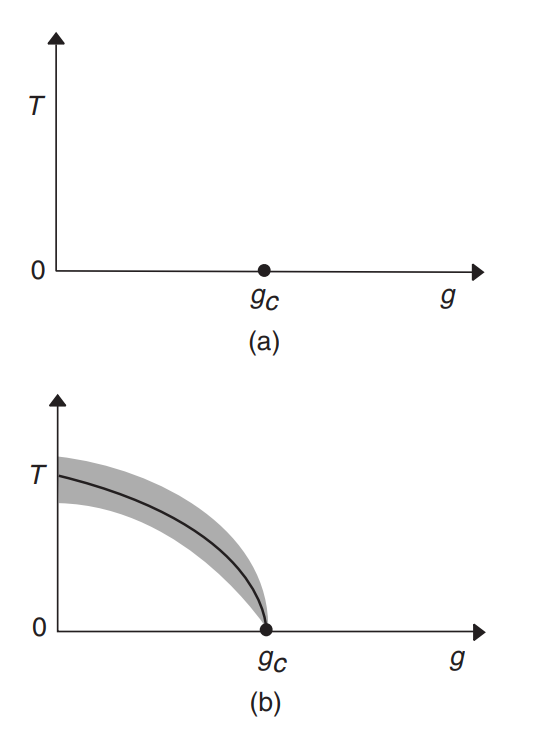
\includegraphics[width=0.5\textwidth]{Figuren/crit/Screenshot from 2021-05-06 15-58-55.png}
    \caption{ Two possible phase diagrams of a system near a quantum phase transition. In both cases there is a quantum critical point at $g = g_c$ and $T = 0$. In (b), there is a line of $T > 0$ second-order phase transitions terminating at the quantum critical point. The theory of phase transitions in classical systems driven by thermal fluctuations can be applied within the shaded region of (b).  Figure and caption taken from \cite{Sachdev1999}. }
    \label{fig:crit:qtran}
\end{figure}



\section{Models}
Models are a simplified mathematical description that captures some relevant physics of more complicated systems. This section introduces some specific models, their relevance and some properties. These models will be used later to benchmark the developed \Gls{TN} cluster expansions.

\subsection{Ising model}\label{models:ising}

The prototypical example of a model in the field of strongly correlated matter is the Ising model. It was first introduced 1925 by Ernest Ising, as a model to capture ferromagnetism. He proved that for a linear chain, there is no phase transition at finite temperatures. He wrongly concluded that this would also be the case in higher dimensions, but it turned out to be one of the deepest and far-reaching problems in the $20^{th}$ century \cite{Taroni2015}.

The Ising model, in essence, assigns an energy contribution to neighbouring spins. These spins sit on a fixed position on a chain (1D) or lattice (2D/3D/...). In classical Ising, the operators in the Hamiltonian all commute with each other. An energy is assigned between neighbouring spins. There is also a contribution for the alignment with an external magnetic field in the same direction. In \Gls{TFI} model, a transversal field is added. The operator measuring the transversal field no longer commutes with the operator measuring the alignment, and hence this is a quantum model. Often, the particles on the grid are spin 1/2 particles, but of course other particles are possible. Many generalizations exist for the Ising model, which will not be discussed her.

\subsubsection{Classical Ising}

The classical Ising model is given by the Hamiltonian
\begin{equation}
    H = -J \left (  \sum_{\Braket{i j }} \sigma_i \sigma_j + h \sum_i \sigma_i \right ),
\end{equation}
where $  \Braket{i j }$ runs over all neighbouring lattice sites. The possible values of $\sigma$ depends on the spin dimension. For spin $1/2$ lattices $\sigma \in {-1,+1}$. g encodes the interaction strength of the external magnetic field. The sign J determines the low temperature ground state. A positive J will tend to align all neighbouring spins at low temperature. This is often called ferromagnetic, because all the aligned spins cause a macroscopic magnetisation. On the other hand, a negative J causes neighbouring spins to have an opposite sign. Depending on the sign of the longitudinal field h, the spins tend to align or antialign with this external field. This lifts the degeneracy of the ground state.

\paragraph{1D}

The classical 1D model was solved analytically by Lens. It can be solved analytically and shows no phase transitions  at finite temperature.

\paragraph{2D}

In 2D, it becomes important to define the lattice. Here, and in the simulations, we will consider a square lattice. This model was famously solved by Lars Onsager in 1944, by using the transfer matrix method. In 2 dimensions, the Ising model has a continuous phase transition at finite temperature. The critical temperature is $T_c = \frac{2 J}{T ln( \sqrt{2}+1)}$. Only the $h=0$ case is solved analytically. For higher dimensions, no analytical solution is known. On different lattices, interesting things can happen. For instance, the ground state of an antiferromagnet on a triangular lattice is not obvious to determine. The spins tend to antialign, but at least 2 of 3 spins on the corner of a triangle have to align. This is called frustration.

\subsubsection{Transverse Field Ising}

As we all know, the real world behaves, certainly at small length and time scales, quantum mechanically. Therefore, it is important to understand how the \acrfull{TFI} model differs from the classical model. In the \Gls{TFI} model, the operators no longer commute with each other. An example is the \Gls{TFI} model given by the  Hamiltonian
\begin{equation}
    \hat{H} = -J \left (  \sum_{\Braket{i j }} \sigma^x_i \sigma^x_j + g \sum_i \sigma^z_i \right ) .
\end{equation}
In the case that $g=0$, this is the classical Ising model (in the $h=0$ case).

\paragraph{1D}
Different to the classical case, the 1D model contains a quantum phase transition at $g=1$. For smaller fields, the ground state has a macroscopic magnetisation, for higher g not. The transition is of type \Cref{fig:crit:qtran} (a). The critical value can be calculated exactly using the Kramers-Wannier duality \cite{Radicevic2018}. The fact that this model has a phase transition can also be understood with \cref{q2cmap}.

\paragraph{2D}

The 2D phase diagram of the \Gls{TFI} model is shown in \cref{2dtisingphasediag}. The notation $\Gamma=g$ is taken in this figure. The classical phase transition is visible at $g=0$. The red dot is the quantum critical point, situated at $ G \approx 3.04  $. A part of this phase diagram will be reproduced in \cref{subsec:qphasediag}.

\begin{figure}[!htbp]
    \center
    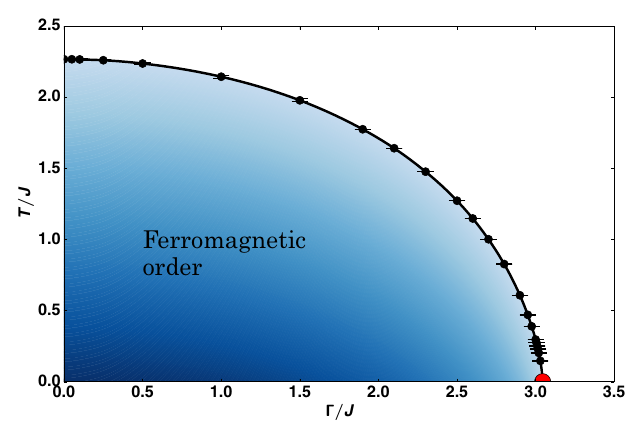
\includegraphics[width=\textwidth]{Figuren/phsyics/2disingphase.png}
    \caption{Phase diagram for 2D \Gls{TFI} model. Figure taken from \cite{Hesselmann2016}.}
    \label{2dtisingphasediag}
\end{figure}

\subsection{Heisenberg}

The Heisenberg model is given by
\begin{equation}
    \hat{H} =  -\left( \sum_{\Braket{i j }} J_x \sigma^z_i \sigma^z_j + J_y \sigma^y_i \sigma^y_j+ J_z \sigma^z_i \sigma^z_j + h \sum_i \sigma^z_i \right ).
\end{equation}
This is a whole class of models, and they have different names depending on the values of $J_{\alpha} $ with $\alpha=x,y,z$. E.g. $J_x = J_y \neq J_z = \Delta$ is called the XXZ model, because the weight for $\sigma^z$ is different. The isotropic version or simply Heisenberg model in the remainder of this thesis, which will be simulated in \cref{chap:results}. The model is
\begin{equation}
    \hat{H} =  -J \left( \sum_{\Braket{i j }} \vec{\sigma} \cdot \vec{\sigma} \right ).
\end{equation}

\subsection{Random}\label{randhamexpl}
It's also possible to construct random Hamiltonians. This is a useful, because it ensures that no special simple structure is present. The single site (which can be thought of as an external field as before) and nearest neighbour Hamiltonians are generated by making Hermitian matrices with random real and complex numbers between -1 and 1. In order to make them comparable, the energy scale is set such that the norm of the Hamiltonian evaluated on 2 sites is 1.

\subsection{Quantum to classical mapping}\label{q2cmap}

In a certain sense, a quantum model in d dimensions can be mapped to a classical model in d+1 dimension. Due to the Lie product formula
\begin{equation}
    e^{A+B} = \lim_{M \to \infty } ( e^{A/M} e^{B/M}  )^M
\end{equation}
we can rewrite the partition function as
\begin{equation}
    \begin{split}
        Z &= \sum_n e^{ - \beta E_n} \\
        &= \sum_n \Braket{n | e^{ - \beta \hat{H} }  | n} \\
        &= \sum_{n_1 \cdots n_M} \Braket{n_1 | e^{ - \beta \hat{H} /M}  | n_2}  \Braket{n_2 | e^{ - \beta \hat{H} /M }  | n_3} \cdots  \Braket{n_{M} | e^{ - \beta \hat{H} /M }  | n_1} \\
        &= \sum_{  n_1 \cdots n_M} \Braket{n_1 | e^{ - \beta \hat{H} /M}  | n_2}  \Braket{n_2 | e^{ - \beta \hat{H} /M }  | n_3} \cdots  \Braket{n_{M} | e^{ - \beta \hat{H} /M }  | n_1} \\
    \end{split}
\end{equation}
where completeness relations $ I = \sum_{n_i}  \ket{ n_i } \bra{ n_i}  $ inserted M times in line 3. This is similar to a path integral. The quantum imaginary time has become a spatial dimension. The quantum model of d dimensions now has the structure of a classical model in d+1 dimensions. In this way, the 2D \Gls{TFI} model can be mapped to the 3D classical Ising model \cite{Hsieh}.

\section{Operator exponentials}

While it is often possible to find exact \Gls{MPO} representation to represent a wide class of Hamiltonians (see \cref{mpo_hamil}), it is much harder to do the same for exponentiated operators. These operators play an important role: they act as time evolution operators for quantum systems $ \ket{\Psi(t)} = \exp( -i \hat{H} t ) \ket{\Psi(0)}$. A very similar operator governs the partition function in statistical mechanics: the probability of finding a system at inverse temperature $\beta = \frac{1}{T}$ in a microstate $i$ is given by $p_i = \exp(  - \beta \hat{H_i} )$. This is often called “imaginary” time, due to the substitution $\beta = i t$. The ability to calculate these operators is essential for understanding the dynamics of a given quantum model, and making contact with real world observations of these systems at finite temperature.

\subsection{Statistical mechanics}\label{subsec:statmech}

The physics of a system in thermodynamic equilibrium can be derived from its partition function Z. The classical formula generalises to a density matrix $\rho$ as follows:
\begin{equation}
    \begin{split}
        Z &= \sum e^{ - \beta E_n} \\
        &= \sum_n \Braket{n | e^{ - \beta \hat{H} }  | n} \\
        &= \Tr( e^{ - \beta \hat{H} } )
    \end{split}
\end{equation}
The first line is the partition function for classical discrete systems. The index n runs over all possible microstates. It is known that the probability to find the system in a given microstate is given by
\begin{equation}
    p_i = \frac{\sum e^{ - \beta E_i}}{Z} .
\end{equation}
A useful quantity is the density matrix $\rho$:
\begin{equation}
    \begin{split}
        \rho &= \sum_j p_i  \Ket{ \Psi_j} \Bra{\Psi_j}   \\
        &= \sum_j \frac{ e^{ - \beta \hat{H} } }{Z}  \Ket{ \Psi_j} \Bra{\Psi_j} .
    \end{split}
\end{equation}
With this notation, the partition function Z and ensemble average of an operator $\hat{X}$ are given by:
\begin{equation}
    \begin{split}
        Z &= \Tr( \rho) \\
        \Braket{X} &= \Tr(\rho \hat{X}) .
    \end{split}
\end{equation}

\subsection{Applications}

\subsubsection{Temporal correlation functions}
The dynamical behaviour of a system can be captured by its dynamic correlation function:
\begin{equation}
    \begin{split}
        C(r,t) &= \left<  \hat{X}(0,0) \hat{X}(r,t)  \right >\\
        &=  \left<  \hat{X}(0)  e^{i \hat{H} t}  \hat{X}(r)  e^{-i \hat{H} t}   \right >
    \end{split}
\end{equation}
This requires time evolution operators $e^{-i \hat{H} t}$.

\subsubsection{Ground state}
One practical way of finding the ground state $ \ket{E_0}$ is to cool down a given random state $ \ket{\Psi(0)}$ to very small T (large $\beta$) \cite{Orus2014}:
\begin{equation}
    \ket{E_0} = \lim_{\beta \rightarrow \infty} \frac{e^{-\beta \hat{H} } \ket{\Psi(0)}  }{  \Braket{ \Psi(\beta) | \Psi(\beta) }  } ,\quad  \ket{\Psi(\beta)} =  e^{-\beta \hat{H} } \ket{\Psi(0)} .
\end{equation}

\subsection{ TN methods}\label{rt_tn_methods}
In the following section I will give a very short review of the current \Gls{TN} methods to simulate real or imaginary time evolution. This overview is mainly based on the review paper \cite{Paeckel2019}.

% https://arxiv.org/pdf/1901.05824.pdf

\subsubsection{Approximations to \texorpdfstring{$ \hat{U}(\delta)$}{U}}
The goal is to approximately make a \Gls{MPO} for a small timestep $\delta$ which gives a new \Gls{MPS} at time $t+\delta$.
\paragraph{\Gls{TEBD}}
Time-evolving block decimation (\Gls{TEBD})  uses the Trotter-Suzuki decomposition. Suppose the chain is split in even and odd sites.
\begin{equation}
    \hat{H} = \hat{H}_{\text{even}}+\hat{H}_{\text{even}}
\end{equation}

\begin{equation}\label{trotter_exp}
    \begin{split}
        \hat{U} = e^{-i \delta \hat{H}_{\text{even}}}  e^{-i \delta \hat{H}_{\text{even}} }e^{-i \delta \left[ \hat{H}_{\text{even}}, \hat{H}_{\text{odd}} \right] }\\
        \approx e^{-i \delta \hat{H}_{\text{even}}}  e^{-i \delta \hat{H}_{\text{even}} }
    \end{split}
\end{equation}
This is now easy to solve: first apply $e^{-i \delta \hat{H}_{\text{even}}}$ for every even bond and afterwards  $e^{-i \delta \hat{H}_{\text{odd}}}$. The error is $O(\delta^2)$ and the number of steps to reach temperature $\beta$ is $\beta / \delta$. The error can be made arbitrarily small. This can be generalised to higher order schemes.

\paragraph{ MPO $W^{I,II}$}
These methods directly use the \Gls{MPO} representation of a certain Hamiltonian
%https://tensornetwork.org/mps/algorithms/timeevo/
This is a more recent method (2015) to construct an \Gls{MPO} first detailed in \cite{Zaletel2015}. The idea is to generalise
\begin{equation}
    1+ \delta \sum_x H_x \rightarrow \prod_x (1+  \delta H_x)
\end{equation}
The error is formally still $O(\delta^2)$, but includes many more terms. The advantages lay in the fact that the form above has an efficient representation as an \Gls{MPO}. \Gls{MPO} $W^I$ and $W^{II}$ are capable of dealing with long-ranged interaction terms which makes it suitable to simulate 2D systems \cite{Paeckel2019}.

\subsubsection{Global Krylov method}

Krylov methods are widely used in linear algebra to calculate eigenvectors. An example is the Lanczos algorithm. These methods are applied to \Glspl{MPS}, but do not fully make use of its structure. For this method, only a \Gls{MPO} representation is needed.

\subsubsection{MPS-local methods}

\paragraph{Local Krylov}
The Krylov methods from the previous paragraph can be adapted to work on a reduced basis.

\paragraph{TDVP} Time-dependent variational principle (TDVP) can be seen as a further development of the local Krylov method. Its also been formulated in as a tangent space algorithm, similar to the \Gls{VUMPS} derivation (\cref{vumps_Deriv}). The Schrödinger equation becomes
\begin{equation}
    i \frac{\partial \ket{ \Psi( A(t) ) }}{\partial t} = \mathcal{P}_{ A ( t) }  H  \ket{ \Psi( A (t) ) } .
\end{equation}
Where the right-hand side is projected on the tangent space, because the left-hand side is also a tangent vector. (See \cite{Vanderstraeten2019}).



\section{Conclusion}
An introduction to phases of matter, and their surprising structure was discussed. 2 models, namely Heisenberg model and the Ising for different dimensions are discussed. The phases for different dimensions are listed. The last section explained the importance of operator exponentials to understand the physics of these models. Competing \Gls{TN} methods to approximate them numerically were very briefly listed.

\chapter{Construction Cluster expansion} \label{chap4}

\section{Introduction}
This is the key chapter of the whole thesis. Here, the novel method to construct the operator $e^{-\beta \hat{H}}$, is explained in detail. The basis of the method was first introduced in \cite{Vanhecke2021}. There are many variations on the same idea. Some of the most notable examples in 1D will be discussed. At this point, no simulation results will be given. These can be found in \cref{chap:results}. The section mentions some objective info about the construction, such as the bond dimension.The 2D construction will generalise the best result from 1D. First, an analogous construction as in 1D will be presented. As can be expected, also some new ideas are needed to capture the rich physics of the models in 2D.The question of how to construct these cluster expansions and other implementation details are reported in \cref{chap5}.

\subsection{Notation}

First, some extra clarification on the notation is needed in order to avoid confusion. In the following, the external legs and virtual level 0 will be omitted. Also, all the physical indices will not be shown. This should not be confused with the diagram earlier.

\begin{equation}
    \mpo{1}{ {0,0}  }{ {"$i$",}  }{ {"$j$",}}{}{{"",}} = \mpob{1}{ {0,0}  }{ {"$i$",}  }{ {"$j$",}}{}{{"",}}
\end{equation}
Each virtual level has its own bond dimension. The bond dimension of level 0 is 0. Two neighbouring sites connected through virtual level 1 are similarly denoted by
\begin{equation}
    \mpo{2}{ {0,1,0}  }{ {"$i_1$","$i_2$"}  }{ {"$j_1$","$j_2$",}}{}{{"",}} =\mpob{2}{ {0,1,0}  }{ {"$i_1$","$i_2$"}  }{ {"$j_1$","$j_1$",}}{}{{"",}}.
\end{equation}
As a reminder, unlabeled incdices such as in
\begin{equation}
    \mpo{3}{ {0,,,0}  }{ {"$i_1$","$i_2$","$i_3$"}  }{ {"$j_1$","$j_2$","$j_3$"}}{}{{"",,}} =\mpob{3}{ {0,,,0}  }{}{}{}{{"",,}}
\end{equation}
implies a summation over all possible virtual levels. A combination is valid if all the separate tensors were defined previously. The goal is capture the exponential of the Hamiltonian operator $\hat{H}$
\begin{equation}
    \hat{H} = \left (  \sum_{<i j>} H^i_2 H^j_2 + \sum_i H^i_1 \right )
\end{equation}
This Hamiltonian consists of 1 and 2 site operators. Of course more general Hamiltonians can also be used. The notation for the contraction of the tensor network will also be used to denote the Hamiltonian evaluated on the given geometry
\begin{alignat}{3}
    H \left( \mpob{3}{ {0,,,0}  }{}{}{}{{"",,}} \right ) = & H_1 &  & \otimes 1   &  & \otimes 1  \nonumber  \\
    +                                                      & 1   &  & \otimes H_1 &  & \otimes 1 \nonumber   \\
    +                                                      & 1   &  & \otimes 1   &  & \otimes H_1 \nonumber \\
    +                                                      & H_2 &  & \otimes H_2 &  & \otimes 1   \nonumber \\
    +                                                      & 1   &  & \otimes H_2 &  & \otimes H_2 \nonumber \\.
\end{alignat}

\subsection{Idea}
This chapter shows the main construction of this dissertation. A cluster expansion is used to approximate $e^{ \hat{H} }$ for every possible geometry. The goal is to make a MPO/PEPO which captures the tensor exponential in the thermodynamic limit.

The main idea is to make an extensive expansion by adding blocks which solve the model exactly on a local patch. Crucially, the expansion is not in the inverse temperature $\beta$ but in the size of the patches. The local patches are separated by a virtual level 0 bond. To make this somewhat more precise, the first steps of the expansion are shown here. The smallest patch, i.e. 1 site,  encodes the exponential of that Hamiltonian
\begin{equation}
    \mpob{1}{ {0,0}  }{}{}{}{{"",}} = \exp \left( -\beta H(\mpob{1}{}{}{}{}{{"",}})   \right).
\end{equation}
If there were no 2 site interactions, this already captures the full diagonalisation. Of course, such a model wouldn't be useful. The next step is to introduce 2 site interactions, where the one site interactions are subtracted from the diagonalised Hamiltonian.
\begin{equation} \label{eq:lev1}
    \begin{split}
        \mpob{2}{ {0,1,0}  }{}{}{}{{"",}}  = \exp -\beta H( & \mpob{2}{ {,,} }{}{}{}{{"",}})  \\
        - &\mpob{2}{ {0,0,0}  }{}{}{}{{"",}}
    \end{split}
\end{equation}
Contraction of larger network lead to many terms, such as
\begin{equation}
    \mpob{10}{ {0,1,0,0,0,1,0,1,0,0,1,0}  }{}{}{}{{"","","","","","","","","","","",}} .
\end{equation}
The beauty of this lays in the fact that disconnected regions(regions separated by level 0) combine in exactly the right way to capture the terms appearing in the series expansion of the exact tensor exponential. Only the terms of the exponential which acts on 3 or more neighbouring sites at once, are not accounted for.

Notice that in \cref{eq:lev1}, 2  new blocks are introduced: $\mpo{1}{ {0,1}  }{ {"$i$",}}{ {"$j$",}}{}{{"",}}$ and of course also $\mpo{1}{ {1,0}}{ {"$i$",}}{ {"$j$",}}{}{{"",}}$. As can be seen, the dimension of virtual level 1 needs to be $d^2$, with d the dimension of physical level. Although different possible constructions already differ in the next step, one more step is added to make te construction and notation clear.
\begin{equation}\label{constr:intro:gen}
    \begin{split}
        \mpob{3}{ {0,1,1,0}  }{}{}{}{{,,,}}  = \exp  -\beta H( &\mpob{3}{ {,,,} }{}{}{}{{,,}})  \\
        - \;&\mpob{3}{ {0,0,0,0}  }{}{}{}{{,,,}}\\
        - \; &\mpob{3}{ {0,1,0,0}  }{}{}{}{{,,,}}\\
        - \; &\mpob{3}{ {0,0,1,0}  }{}{}{}{{,,,}}\\
        =\exp  -\beta H( &\mpob{3}{ {,,,} }{}{}{}{{,,}})\\
        - \; &\mpob{3}{ {,,,}  }{}{}{}{{,,,}}\\
    \end{split}
\end{equation}
This is called an cluster expansion of order 3, because there are 3 connected sites solved exactly. The right-hand side of \cref{constr:intro:gen} can be ommited, as it is just evaluating the exponentiated Hamiltonian on the same geometry as the left hand side and substructing all possible contractions of the blocks which were added previously. This very compact notation will be able to capture the essence of the different constructions. Because it is important for the remainder of the chapter, it is stressed that for an equation similar to
\begin{equation}
    \boxed{\mpob{3}{ {0,1,1,0}  }{}{}{}{{,,,}} },
\end{equation}
the right-hand side of \cref{constr:intro:gen} is implied. In the following section, different types will be discussed. For every chain lenght, a new block is defined. This could be done in numerous ways. The different types list some ways to do this.

\section{Construction MPO}\label{H4_mpo_cons}

\subsection{Type A}
This type was originally proposed in \cite{Vanhecke2021}. The first few blocks in the expansion are the following:

\begin{equation}
    \begin{split}
        &\mpob{1}{ {,}  }{}{}{}{{,,}} \\
        &\mpob{2}{ {,"1",}  }{}{}{}{{,,}}\\
        &\mpob{3}{ {,"1","1",}  }{}{}{}{{,,,}}\\
        &\mpob{4}{ {,"1","2","1",}  }{}{}{}{{,,,,,}}\\
        &\mpob{5}{ {,"1","2","2","1",}  }{}{}{}{{,,,,,}}\\
    \end{split}
\end{equation}

The following types of blocks appear in the cluster expansion

\mpo{1}{ {"n","m"}  }{}{}{}{},\mpo{1}{ {"m ","n"}  }{}{}{}{} and \mpo{1}{ {"n","n"}  }{}{}{}{} with $n \in \mathbb{N}_0$ and $m=n-1$.

The $O^{n n}$ block is in defined for a chain with an odd number of sites. The contraction of $O^{n m }$ and $O^{m n} $ is defined by for a chain with even order. The decomposition is defined up to a gauge transformation.

\subsubsection{Dimension}

In this scheme, virtual level n has dimension $d^n$. Of course, this dimension can be lowered if some error is allowed for the longest chain.

\subsubsection{discussion}

Type A can form long chains, which where not explicitly optimised for. The question arise whether this will results in accurate results for cyclic systems or not.

\subsection{Type B}

Type B only contains blocks of the following form; $O^{m n}$ and $O^{n 0}$.The first few blocks are:
\begin{equation}
    \begin{split}
        &\mpob{1}{ {,}  }{}{}{}{{,,}} \\
        &\mpob{2}{ {,"1",}  }{}{}{}{{,,}}\\
        &\mpob{3}{ {,"1","1",}  }{}{}{}{{,,,}}\\
        &\mpob{4}{ {,"1","2","3",}  }{}{}{}{{,,,,,}}\\
        &\mpob{5}{ {,"1","2","3","4",}  }{}{}{}{{,,,,,}}\\
    \end{split}
\end{equation}

\def \rhs{\expH{2}{ $L_{m}^{-1}  M_{n+1} $ }{{"$i_n$","$i_{n+1}$"}}{{"$j_n$","$j_{n+1}$"}}{{"m","0"}}  }
\begin{equation}
    \begin{split}
        \mpo{2}{ {"m","n","0"}  }{ { "$i_n$","$i_{n+1}$"}}{ { "$j_n$","$j_{n+1}$"}}{}{} =  U^n  \Sigma V^{\dagger}\\
    \end{split}
\end{equation}

The following split is made: $O^{m n} \cong U^n$ and $O^{n 0} \cong  \Sigma V^{\dagger}$. In this way the left inverse exists and doesn't need any calculation: $O^{m n} = U^{\dagger}$.

\subsubsection{dimension} From the construction the bond dimension grows from the left to the right. For the last step, there are only $d^2$ non zero singular values.  Each steps adds $d^2$ to the dimension.
For the last step, only $d^2$ non zero singular values need to be keeped. With the following natation:
\begin{equation}
    \begin{split}
        \mpo{1}{ {"m","n"}  }{ { "\(i\)",}}{ { "$j$",}}{}{} &= A^m_{ (\alpha i j ) \beta} \\
        \mpo{1}{ {"n","0"}  }{ { "$i$",}}{ { "$j$",}}{}{} &= B^n_{ (\alpha i j ) \beta} \\
    \end{split}
\end{equation}
The bond dimension of lower virtual levels can be reduced if we can solve the following equations simultaneously:

Then the MPO doesn't change if there are matrices $A'^{n}$, $A'^{n+1}$ and $B'^{n}$ such that
\begin{equation}
    \begin{split}
        S=A^{m} A^{n} &= A'^{m} A'^{n} \\
        T=A^{m} B^{n} &= A'^{m} B'^{n} \\
    \end{split}
\end{equation}
Such matrices with optimal bond dimension can be found with generalised SVD. Generalised SVD decomposes 2 matrices as follows:
\begin{equation}
    \begin{split}
        S^{\dagger} = (U \Sigma_1) Q^{\dagger} \\
        T^{\dagger} = (V \Sigma_2) Q^{\dagger}
    \end{split}
\end{equation}
The new bond dimension is the $\dim{n'} =d^2 \cdot \min( \dim{n-1}, \dim (n+1) )$.  This is higher than the dimension of type A.

\subsubsection{Discussion}
The bond dimension is larger than type A, but the long chains from A are absent. The left inverse is always well defined and doesn't need any computation, because hermitian matrix U can be inverted easily. One major drawback is that for long chains, the virtula bonds are very large before they can be shrunk with the gsvd procedure.

\subsection{Type C}

This type implements the same strict type as Type B, but in a different way. No calculation is involved, except the calculation of the the exponentiated hamiltonian to certain order. The following kind of MPO strings are allowed:

\begin{equation}
    \begin{split}
        &\mpob{1}{ {,}  }{}{}{}{{,,}} \\
        &\mpob{2}{ {,"1",}  }{}{}{}{{,,}}\\
        &\mpob{3}{ {,"1'","1'",}  }{}{}{}{{,,,}}\\
        &\mpob{4}{ {,"1''","2''","3''",}  }{}{}{}{{,,,,,}}\\
        &\mpob{5}{ {,"1'''","2'''","3'''","4'''",}  }{}{}{}{{,,,,,}}\\
    \end{split}
\end{equation}
and so forth. All but one MPO elements are chosen to be the identity matrix. The middle one is the exponentiated hamiltonian with reshaped legs.

\subsubsection{discussion}
As can be expected from the construction, the bond dimension grows very fast. This type is just as precise as Type B.

\subsection{Type D}

This type uses a differemt setup which tries to capture the best of both Type A and B. Type  could handle long range correlation better because of the introuction of $O^{n n}$, but the inverse was not necesarily well defined. Type B had well conditioned inverses, but performed in most of the cases worse. The block appearing in type D are as follows:

\mpo{3}{{"m","n","n","m"}}{{,"-",}}{{,"-",}}{}{{"O","$D_n$","O"}} and \mpo{1}{{"n","n"}}{}{}{}{}

Similar to type A,

\def \rhs{\expH{2}{ $L_{n}^{-1}  M_{2n+2}  R_{n}^{-1}$ }{}{}{{"n","n"}}  }
\begin{equation}
    \begin{split}
        \mpo{3}{{"m","n","n","m"}}{{,"-",}}{{,"-",}}{}{{"O","$D_n$","O"}} &= \rhs \\
        &= U \Sigma V^{ \dagger}
    \end{split}
    \label{eq_nmn_level}
\end{equation}

Matrix $D_n$ is the singular value diagonal matrix devided by a normalisation factor $\phi$. Both U and V are multiplied by $  \sqrt{\phi} $.

\subsubsection{discussion}
It's not completely clear what the values of $\phi$ should be.  If $\phi$ is to large, large chains are not surpressed. If phi is to small, the $O^{n n}$ blocks will become large and hence the chain will diverge again. A reasonable value is the sum of the singular values. Other combination could be tried.

\subsubsection{matrisation}
The cost of this type lies in the fact that it has no compact way of casting it to a matrix. The following works, but has quite a large dimension:

\begin{tabular}{ccc|cc|cc|cc}
    $O_{00}$               & $O_{01} $   &             & $-2  O_{01}$ &                & $ O_{01}$ &             & $ O_{01}  D_1^{1/2}$           &                                \\
    ${O_{10}}$             &             & ${ O_{12}}$ &              & $-2 { O_{12}}$ &           & ${ O_{12}}$ &                                &                                \\
                           & ${ O_{21}}$ &             &              &                &           &             &                                &                                \\
    \hline
    ${O_{10}}$             &             &             &              &                &           &             &                                &                                \\
                           & ${ O_{21}}$ &             &              &                &           &             &                                &                                \\
    \hline
    ${ O_{10}}$            &             &             &              &                & $O_{11}$  &             &                                &                                \\
                           & ${ O_{21}}$ &             &              &                &           & $O_{22}$    &                                &                                \\
    \hline
    $ D_1^{1/2} { O_{10}}$ &             &             &              &                &           &             &                                & $D_1^{-1/2} O_{12}  D_2^{1/2}$ \\
                           &             &             &              &                &           &             & $ D_2^{1/2} O_{21} D_1^{-1/2}$                                  \\\end{tabular}

\subsection{Type E}

Again, this is a strict variant which needs exactly twice the bond dimension of type A. The idea is to split every chain in a left and a right part. For the left part, the numbers increase while right part they decrease. This construction carries over well to higher dimensions. The first few blocks are:
\begin{equation}
    \begin{split}
        &\mpob{1}{ {,}  }{}{}{}{{,,}} \\
        &\mpob{2}{ {,"1",}  }{}{}{}{{,,}}\\
        &\mpob{3}{ {,"1","1'",}  }{}{}{}{{,,,}}\\
        &\mpob{4}{ {,"1","2","1'",}  }{}{}{}{{,,,,,}}\\
        &\mpob{5}{ {,"1","2","2'","1'",}  }{}{}{}{{,,,,,}}\\
    \end{split}
\end{equation}
The construction is very similar to type A

\subsection{Type F}

The idea behind this type is very similar to type D. The blocks look as follows:
\begin{equation}
    \begin{split}
        &\mpob{1}{ {,}  }{}{}{}{{,,}} \\
        &\mpob{2}{ {,"1'",}  }{}{}{}{{,,}}+\mpob{2}{ {,"1'",}  }{}{}{}{{,,}}\\
        &\mpob{3}{ {,"1","1",}  }{}{}{}{{,,,}}\\
        &\mpob{4}{ {,"1","2","1",}  }{}{}{}{{,,,,,}}+\mpob{4}{ {,"1","2'","1",}  }{}{}{}{{,,,,,}}\\
        &\mpob{5}{ {,"1","2","2","1",}  }{}{}{}{{,,,,,}}\\
    \end{split}
\end{equation}

The  blocks $O^{n-1,n}$ and $O^{n,n-1}$ unitary matrices from the svd decomposition, scaled by the largest singular value. The blocks $O^{n-1,n'}$ and $O^{n',n-1}$ are then used to actually solve the problem for the given chain. In the next step, $O^{n,n}$ is added as usual. The idea here is once again to keep this block small, in order to not cuase any divergences.

\subsection{Conclusion}

Many 1D constructions are discussed here. They can be roughly divided in 2 groups. B, C and E are strict variants, meaning only the explicitly constructed blocks will appear in the final expansion. As a consequence, they have exactly the same predictive power. While B has some advantageous properties such as its final bond dimension and well-defined inverses, type E will be used in the results chapter due to its simplicity and scalability. It also generalises well to 2D, in contrast to type B.

The second category are the unstrict types. Type A has the lowest possible bond dimension to exactly represent a chain of a given length. One hurdle to be overcome are the badly conditioned inverses, when implemented naively. Types D and F try to remedy this. D scales very badly with the maximum number of sites, and has a construction which doesn't fit in with the simple diagrams. The construction was only implemented in 1D code due to this. This type won't be reported, and has a similar performance to type F.

In short, type A, E and F will be reported in \cref{sec:results1d}.

\section{Construction PEPO}\label{H4_pepo_cons}
While there were some interesting choices in the 1D construction, the number of possibilities in 2D is virtually limitless. The focus will mainly be to generalise type A to 2D. As can be expected, the construction starts off quite similar. The following blocks are called 'Linear', due to the way they will be solved.

\subsection{Linear blocks}\label{subsec:lin_block_Def}

\begin{equation}
  O^{0 0 0 0 }= \mpob{1}{ {,}  }{}{}{}{{,,}} = \vcenter{ \hbox{ \pepob{4}{3}{{
            "-","-","-",
            "-","0","0",
            "-","-","-"}}{{
            "-","-",
            "-","-",
            "0","0",
            "-","-"}}{{
            1,1,4,1,
            1,4,12,4,
            1,1,4,1}} }}
\end{equation}
This block now contains 2 physical indices and 4 virtual legs. Similar to 1D construction, the 0 legs and physical indices are hidden. The next order 2 blocks are
\begin{equation}\label{2dblocksorder2}
  \pepob{2}{2}{{"1",,}}{{,,}}{{0,0,1,1}}  \pepob{2}{2}{{,,}}{{"1",,}}{{0,1,0,1}}.
\end{equation}
From 3 blocks onwards, the number of extra blocks start to increase:
\begin{equation}
  \begin{split}
    \pepob{2}{2}{{"1","1",}}{{"1","1",}}{{0,0,0,1}} \;  \pepob{2}{2}{{"1","1",}}{{"1","1",}}{{0,0,1,0}} \; \pepob{2}{2}{{"1","1",}}{{"1","1",}}{{0,1,0,0}} \; \pepob{2}{2}{{"1","1",}}{{"1","1",}}{{1,0,0,0}}\\
    \pepob{3}{2}{{"1","1","1","1"}}{{"1","1","1","1"}}{{0,0,0,1,1,1}} \; \pepob{2}{3}{{"1","1","1","1"}}{{"1","1","1","1"}}{{0,1,0,1,0,1}}
  \end{split}
\end{equation}
Of course, besides linear blocks also $\perp$ and + shapes need to be constructed to fully capture the model.
\begin{equation}
  \pepob{3}{2}{{"1","1","1","1"}}{{"1","1","1","1"}}{{0,0,0,1,0,1}}
\end{equation}
\begin{equation}
  \pepob{3}{3}{{"1","1","1","1","1","1",}}{{"1","1","1","1","1","1",}}{{1,0,1,0,0,0,1,0,1}}
\end{equation}
Here, and in the following, care has to be taken in which order the blocks are added. In general, every block which fits in the given block needs to be constructed beforehand. The construction continues by introducing a virtual level 2 as before:
\begin{equation}
  \mpob{4}{ {,"1","2","1",}  }{}{}{}{{,,,,,}}
\end{equation}
Again, 2 blocks are introduced. For other variations of the linear chain, only one block needs to be solved
\begin{equation}
  \begin{split}
    &\pepob{3}{2}{{"2","1","2","1",}}{{"1","1","1",,}}{{0,1,1,0,0,0}}\\
    &\pepob{3}{2}{{"2","1",,}}{{"1","1",,,}}{{0,0,0,0,1,1}} .
  \end{split}
\end{equation}
Due to the way they are constructed, the error for every linear chains of a given length will be the same as in the 1D case. Once again, all possible $\perp$  and + blocks are created. Some of these blocks are shown here:
\begin{equation} \label{eq:cross_terms:order4}
  \vcenter{\hbox{ \pepob{4}{3}{{
            "-","-","-",
            "1","2","1",
            "-","-","-"}}{{
            "-","-",
            "-","-",
            "1","-",
            "-","-"}}{{
            1,1,0,1,
            0,0,0,0,
            1,1,1,1}}  \pepob{4}{3}{{
            "-","-","-",
            "1","2","1",
            "-","-","-"}}{{
            "-","-",
            "-","-",
            "1","1",
            "-","-"}}{{
            1,1,0,1,
            0,0,0,0,
            1,1,0,1}} }}
\end{equation}
\begin{equation} \label{eq:cross_terms:order5}
  \begin{split}
    &\pepob{5}{3}{{
          "-","-","-","-",
          "1","2","2","1",
          "-","-","-","-"}}{{
          "-","-",
          "-","-",
          "1","-",
          "-","-",
          "-","-"}}{{
          1,1,0,1,1,
          0,0,0,0,0,
          1,1,1,1,1}}  \pepob{5}{3}{{
          "-","-","-","-",
          "1","2","2","1",
          "-","-","-","-"}}{{
          "-","-",
          "-","-",
          "1","1",
          "-","-",
          "-","-"}}{{
          1,1,0,1,1,
          0,0,0,0,0,
          1,1,0,1,1}} \\
    &\pepob{5}{4}{{
          "-","-","-","-",
          "-","-","-","-",
          "1","2","2","1",
          "-","-","-","-"}}{{
          "-","-","-",
          "-","-","-",
          "1","2","1",
          "-","-","-",
          "-","-","-"}}{{
          1,1,0,1,1,
          1,1,0,1,1,
          0,0,0,0,0,
          1,1,1,1,1}} \pepob{5}{4}{{
          "-","-","-","-",
          "-","-","-","-",
          "1","2","2","1",
          "-","-","-","-"}}{{
          "-","-","-",
          "-","-","-",
          "1","2","1",
          "-","-","-",
          "-","-","-"}}{{
          1,1,0,1,1,
          1,1,0,1,1,
          0,0,0,0,0,
          1,1,0,1,1}} \\
    &\pepob{5}{5}{{
          "-","-","-","-",
          "-","-","-","-",
          "1","2","2","1",
          "-","-","-","-",
          "-","-","-","-"}}{{
          "-","-","-","-",
          "-","-","-","-",
          "1","2","2","1",
          "-","-","-","-",
          "-","-","-","-"}}{{
          1,1,0,1,1,
          1,1,0,1,1,
          0,0,0,0,0,
          1,1,0,1,1,
          1,1,0,1,1}} \; .
  \end{split}
\end{equation}
For each block shown, there are still multiple permutations of the legs possible. Due to the way the virtual level 1 blocks were added, all variations are captured, such as
\begin{equation}
  \vcenter{\hbox{ \pepob{4}{3}{{
            "-","-","-",
            "1","2","1",
            "-","-","-"}}{{
            "-","-",
            "-","1",
            "1","-",
            "-","-"}}{{
            1,1,0,1,
            1,0,0,0,
            1,0,1,1}} }} \; .
\end{equation}
It is clear that a completely automated solver is needed to construct all these different blocks. From here on, the construction generalises easily to higher block numbers, and to higher dimensions. The difference between \cref{eq:cross_terms:order4} and the blocks in \cref{eq:cross_terms:order4} is the longest chain that fit in the geometry. For \cref{eq:cross_terms:order4}, only chains of order 4 are present, while  \cref{eq:cross_terms:order5} has chains of length 5. It seems that when a virtual level is present, it is most advantageous to create both the even and odd order chains, but this will not be the case when a virtual level is truncated.

\subsection{Loops}

While the blocks above certainly encode many finite-size patches, there are still quite some patches that need to be encoded. The simplest case is a 1 square loop.
\begin{equation}
  {\pepob{2}{2}{{"","",}}{{"","",}}{{0,0,0,0}}}
\end{equation}
It is clear that this problem cannot be solved with the techniques from the previous section. The square loop needs a new virtual level $\alpha$. In general, all the loop levels will be named with Greek letters for convenience. The simplest choice for the loop is:
\begin{equation}\label{tikzfig:plaquetter}
  {\pepob{2}{2}{{"$\alpha$","$\alpha$",}}{{"$\alpha$","$\alpha$",}}{{0,0,0,0}}}
\end{equation}
At this point all blocks of order 4 are solved.

\subsubsection{Single extensions}
The loops need to be connected to the linear blocks. One way to do this is as
\begin{equation}
  \vcenter{\hbox{ \pepob{5}{3}{{
            "-","-","-","-",
            "-","1","$\alpha$","-",
            "-","-","$\alpha$","-"}}{{
            "-","-",
            "-","-",
            "-","$\alpha$",
            "-","$\alpha$",
            "-","-"}}{{
            1,1,1,1,1,
            1,0,0,0,1,
            1,1,0,0,1}} }} .
\end{equation}
With the given blocks, the following combination is also possible
\begin{equation}
  \vcenter{\hbox{  \pepob{5}{3}{{
            "-","-", "-",     "-",
            "-","1","$\alpha$","-",
            "-","-","$\alpha$","-"}}{{
            "-","-",
            "-","-",
            "-","$\alpha$",
            "1","$\alpha$",
            "-","-"}}{{
            1,1,1,0,1,
            1,0,0,0,1,
            1,1,0,0,1}} }}.
\end{equation}
This results in very large errors, and it would require many more blocks to be added in order to counteract this. Luckily, there are many possibilities in 2D. One example is
\begin{equation}\label{eq:loop_1ext}
  \vcenter{\hbox{ \pepob{5}{3}{{
            "-","-", "-",     "-",
            "-","1","$\beta$","-",
            "-","-","$\alpha$","-"}}{{
            "-","-",
            "-","-",
            "-","$\gamma$",
            "-","$\alpha$",
            "-","-"}}{{
            1,1,1,1,1,
            1,0,0,0,1,
            1,1,0,0,1}}}} \; .
\end{equation}
The pieces with $\beta$ and $\gamma$ are only rotated, and not for instance switched. Different to the $\alpha$-cornerpiece, only a loop with one extension at is possible. Of course, there is no need to stop here, the following blocks can now be constructed easily
\begin{equation}\label{eq:s_loop_ext}
  \vcenter{\hbox{  \pepob{5}{3}{{
            "-","-", "-",     "-",
            "1","2","$\beta$","-",
            "-","-","$\alpha$","-"}}{{
            "-","-",
            "-","-",
            "-","$\gamma$",
            "-","$\alpha$",
            "-","-"}}{{
            1,1,1,1,1,
            0,0,0,0,1,
            1,1,0,0,1}} \quad \pepob{5}{3}{{
            "-","-", "-",     "-",
            "-","1","$\beta$","-",
            "-","-","$\alpha$","-"}}{{
            "-","-",
            "-","-",
            "1","$\gamma$",
            "-","$\alpha$",
            "-","-"}}{{
            1,1,0,1,1,
            1,0,0,0,1,
            1,1,0,0,1}} }} \; .
\end{equation}

\subsubsection{Double extensions}

It seems as if one of the corner pieces can be used as follows
\begin{equation}
  \vcenter{\hbox{  \pepob{5}{3}{{
            "-","-", "-",     "-",
            "-","1","$\beta$","-",
            "-","-","$\alpha$","-"}}{{
            "-","-",
            "-","-",
            "-","$\gamma$",
            "1","$\alpha$",
            "-","-"}}{{
            1,1,1,0,1,
            1,0,0,0,1,
            1,1,0,0,1}} }} \; ,
\end{equation}
But in order to make a meaningful change in the residual error, the bond dimension of both $\alpha$ and $\beta$ needs to be enlarged significantly. It is more advantageous to introduce yet another level $\delta$, which forms the link between the 2 parts. As both corner tensors can be optimised at once, the total bond dimension is lower than for the previous suggestion, but still larger than the dimensions of the other loop levels.

\begin{equation}
  \pepob{5}{3}{{
        "-","-", "-", "-",
        "-","1","$\delta$","-",
        "-","-","$\alpha$","-"}}{{
        "-","-",
        "-","-",
        "-","$\gamma$",
        "1","$\beta$",
        "-","-"}}{{
        1,1,1,0,1,
        1,0,0,0,1,
        1,1,0,0,1}}
\end{equation}

\subsubsection{Larger loops}
One question which comes to mind is where the focus should be for the construction. Making blocks for all possible single loop extensions comes at an increasing cost in total bond dimension. From a physics point of view, the model will be better approximated when the smallest non-solved patch is solved by introducing new blocks. On the other hand, the already included blocks may cause an error which was not present before the blocks were introduced. An example is the different + blocks which connect upon themselves in the following shapes
\begin{equation}
  \vcenter{\hbox{  \pepob{5}{3}{{
            "","","","",
            "","","","",
            "","","",""}}{{
            "","",
            "","",
            "","",
            "","",
            "",""}}{{
            1,0,0,1,1,
            1,0,0,0,1,
            1,1,0,0,1}}  }}  \quad   \vcenter{\hbox{   \pepob{5}{3}{{
            "","","","",
            "","","","",
            "","","",""}}{{
            "","",
            "","",
            "","",
            "","",
            "",""}}{{
            1,1,0,0,1,
            1,0,0,0,1,
            1,0,0,1,1}} }} .
\end{equation}
One way to solve this, without breaking the rotation pattern of $\beta$ and $\gamma$, is
\begin{equation}\label{tbtrectblock}
  \pepob{5}{3}{{
        "","$\alpha$","","",
        "","$\beta$","$\beta$","",
        "","","$\alpha$",""}}{{
        "","",
        "$\alpha$","",
        "$\gamma$","$\gamma$",
        "","$\alpha$",
        "",""}}{{
        1,0,0,1,1,
        1,0,0,0,1,
        1,1,0,0,1}}
\end{equation}
Many more blocks were tried, such as blocks to solve
\begin{equation}
  \pepob{5}{3}{{
        "","","","",
        "","","","",
        "","","",""}}{{
        "","",
        "","",
        "","",
        "","",
        "",""}}{{
        1,1,1,1,1,
        1,0,0,0,1,
        1,0,0,0,1}}.
\end{equation}
The tried extensions mostly failed, including the double extensions and larger loops discussed here. In \cref{subsec:results:loops_and_ext}, it is explained why the results of these additions were not very reliable.

\subsubsection{Bond dimension}

While for the linear blocks it is clear what the bond dimension should be, this is not the case for the graphs with loops. This optimal dimension cannot be directly determined for a tensor ring decomposition \cite{Zhao2016}, but needs to be deduced during the construction. In practice, a bond dimension of 6 is enough to fully solve \cref{tikzfig:plaquetter} (for physical dimension 2). For \cref{eq:loop_1ext}, at least bond dimension 8 is required for $\beta$ and $\gamma$ level. This is also sufficient to solve longer extensions and multiple extensions from one corner.



\section{Symmetry}\label{sec:symm}
When the linear blocks are constructed without symmetry considerations, quite some blocks are required. For any one of the 4 legs, the virtual level can range from 1 to M, with M the maximum virtual bond dimension. This results in $(M+1)^4$ blocks. Another possibility is to restrict all equations further by imposing rotation symmetry of the PEPO legs:
\begin{equation}\label{eq:rotsympepo}
  \vcenter{ \hbox{\pepob{2}{2}{{"1","1"}}{{"1","1"}}{{
            0,4,
            1,1,
          }} } } =     \vcenter{ \hbox{\pepob{2}{2}{{"1","1"}}{{"1","1"}}{{
            4,0,
            1,1,
          }} } } = \vcenter{ \hbox{\pepob{2}{2}{{"1","1"}}{{"1","1"}}{{
            4,1,
            0,1,
          }} } }= \vcenter{ \hbox{\pepob{2}{2}{{"1","1"}}{{"1","1"}}{{
            0,1,
            4,1,
          }} } }
\end{equation}
In this way, only the blocks unique up to a permutation of the legs need to be solved. More generally, the following rotation symmetry on the PEPO level is imposed
\begin{equation}
  \vcenter{ \hbox{ \pepob{4}{3}{{
            "-","-","-",
            "-","a","c",
            "-","-","-"}}{{
            "-","-",
            "-","-",
            "d","b",
            "-","-"}}{{
            1,1,4,1,
            1,4,12,4,
            1,1,4,1}} }} = \vcenter{ \hbox{ \pepob{4}{3}{{
            "-","-","-",
            "-","b","d",
            "-","-","-"}}{{
            "-","-",
            "-","-",
            "a","c",
            "-","-"}}{{
            1,1,4,1,
            1,4,12,4,
            1,1,4,1}} }} \; .
\end{equation}


\section{Conclusion}
The cluster expansions are introduced here for both a 1D and 2D setting. This can be represented with some very compact notation, as explained in \cref{constr:intro:gen}. The best 1D type, namely A, was used as an inspiration for 2D cluster expansion. For 2D, mainly the linear blocks, loops and single extension will be important in the results.

\chapter{Framework implementation}\label{chap5}

%“Experience is the name everyone gives to their mistakes.” – Oscar Wilde

% \epigraph{An expert is a person who has made all the mistakes that can be made in a very narrow field}{Niels Bohr}

\epigraph{Experience is the name everyone gives to their mistakes.}{Oscar Wilde}

\section{Introduction}
The construction was explained in the previous chapter, but there is a lot of work that needs to be done to go from an idea to a working implementation in MATLAB. The framework to do these calculations was programmed starting from scratch during the course of this thesis. This chapter aims to show some work involved. First, the solvers, used to numerically extract the new blocks introduced for each equation in the previous chapter, are explained. There are 3 different solvers: a linear solver based on matrix inversion, a nonlinear solver based on MATLAB's fsolve and a sequential linear solver, which iteratively solves each occurring tensor with the linear solvers takes a step in that direction. The solvers need to be as fast as possible, numerically stable and accurate. The optimisation section gives more details about the framework in general. A section is dedicated to the code for generating the phase diagrams reported in the results chapter.  The source code is freely available, and \cref{sec:H5:source_code} shows very briefly how the code is structured. Finally, some limitations and possibilities relating to the framework are discussed.

\section{Solvers} \label{sec:framework_impl}
The construction can be written down quite compactly as done in the previous section, but actually implementing the code in full generality is somewhat more complex. In practice, the 1D and 2D implementation were performed separately. Where a part of the code but mainly the ideas and lessons learned from 1D where taken to the 2D code. Of course, the 1D construction is just a subset of the 2D implementation. In fact, the 2D implementation even outperforms the 1D implementation for reasons with will be explained later. The main focus of this chapter will go to the 2D implementation. At the end some particular optimisations in 1D will be highlighted.

Solving the blocks introduced in the previous sections need 2 different approaches. The graphs of the maps can be split in 2 groups. The first one, considers problems where there are no loops and at most one node with more than 2 legs Examples include:
$\pepob{3}{2}{{"1","1","1","1"}}{{"1","1","1","1"}}{{0,0,0,1,0,1}}$ and $\mpob{4}{ {,"1","2","1",}  }{}{}{}{{,,,,,}}$.
These will be reduced to a standard matrix problem, and solve with matrix (pseudo-) inversion.

The other group, of course, constitutes the nonlinear problems. This includes every problem where a block (or rotated version) occurs more than once, problems which include loops, ...

\subsection{Linear solver} \label{subsec:linear_solver}

\todo{make tikz figures}

\subsubsection{Full inverse}

The linear solver is a general purpose block solver which reduces the problem to a set of linear matrix equations. Linear block consist of a tree structure, where the new block is the root of the tree, and all the branches need to be inverted.  Let $ I^m = (i^1_1 i^1_2 \cdots i^1_{n_1})$ be all the physical indices of one leg m and $\alpha^m$ the index between leg m and unknown matrix X. Then the problem can in general, after some tedious tensor leg bookkeeping, be rewritten in the following form
\begin{equation}\label{axb}
    \begin{split}
        &A_{ I^1  I^2 \cdots I^n \alpha^1 \alpha^2 \cdots \alpha^m   } X_{ \alpha^1 \alpha^2 \cdots \alpha^m j  } \\
        = &B_{  I^1  I^2 \cdots I^m   j } .
    \end{split}
\end{equation}
Here $i^M_N$ has the following meaning: M numbers the different legs or branches of the tree, N number of sites of the leg and i numbers the bra and ket states and has dimension $d^2$. Hence, the bond dimension of $I_n= d^{2 n_m }$.

\def \pepoat {\begin{tikzpicture}[baseline=0.5]

        \def \legLength { 0.8}
        \def \radius {0.1}

        \pgfmathsetmacro{\step}{2*\radius+ \legLength} % 1
        \pgfmathsetmacro{\legpos}{\radius+\legLength} %0.9

        \node[draw,circle, radius=\radius] (O0) at (0,0) {};

        \node[draw, circle,radius=\radius] (L1) at (-1,0) {};
        \node[draw, circle,radius=\radius] (L2) at (-2,0) {};
        \node[draw, circle,radius=\radius] (L3) at (-3,0) {};

        \node[draw, circle,radius=\radius] (U1) at (0,1) {};
        \node[draw, circle,radius=\radius] (U2) at (0,2) {};

        \node[draw, circle,radius=\radius] (D1) at (0,-1) {};

        \node[draw, circle,radius=\radius] (R1) at (1,0) {};

        \draw (O0) -- (L1);
        \draw (L2) -- (L1);
        \draw (L2) -- (L3);

        \draw (O0) -- (U1);
        \draw (U2) -- (U1);

        \draw (O0) -- (R1);

        \draw (O0) -- (D1);

        \draw (O0.center) -- ++(0.2,0.2);
        \draw (L1.center) -- ++(0.2,0.2);
        \draw (L2.center) -- ++(0.2,0.2);
        \draw (L3.center) -- ++(0.2,0.2);
        \draw (U1.center) -- ++(0.2,0.2);
        \draw (U2.center) -- ++(0.2,0.2);
        \draw (R1.center) -- ++(0.2,0.2);
        \draw (D1.center) -- ++(0.2,0.2);

    \end{tikzpicture}}

\def \blockat {  \begin{tikzpicture}[baseline=0.5]

        \def \legLength { 0.8}
        \def \radius {0.1}

        \pgfmathsetmacro{\step}{2*\radius+ \legLength} % 1
        \pgfmathsetmacro{\legpos}{\radius+\legLength} %0.9

        \node[draw=none] (O0) at (0,0) {};

        \node[draw=none] (L1) at (-1,0) {};
        \node[draw=none] (L2) at (-2,0) {};
        \node[draw=none] (L3) at (-3,0) {};

        \node[draw=none] (U1) at (0,1) {};
        \node[draw=none] (U2) at (0,2) {};

        \node[draw=none] (D1) at (0,-1) {};

        \node[draw=none] (R1) at (1,0) {};

        \draw (O0.center) -- ++(0.2,0.2);
        \draw (L1.center) -- ++(0.2,0.2);
        \draw (L2.center) -- ++(0.2,0.2);
        \draw (L3.center) -- ++(0.2,0.2);
        \draw (U1.center) -- ++(0.2,0.2);
        \draw (U2.center) -- ++(0.2,0.2);
        \draw (R1.center) -- ++(0.2,0.2);
        \draw (D1.center) -- ++(0.2,0.2);

        \draw (-3.3,0.3)--(-0.3,0.3) -- (-0.3,2.3)--(0.3,2.3)
        -- (0.3,0.3) -- (1.3,0.3) -- (1.3,-0.3) -- (0.3,-0.3)
        -- (0.3,-1.3) -- (-0.3, -1.3) -- (-0.3,-0.3) -- (-3.3,-0.3) -- cycle;

    \end{tikzpicture}}

\def \pepobt {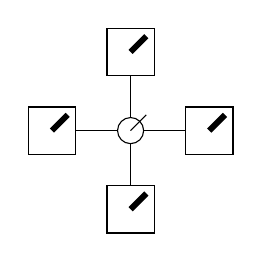
\begin{tikzpicture}[baseline=0.5]

        \def \legLength { 0.8}
        \def \radius {0.1}

        \pgfmathsetmacro{\step}{2*\radius+ \legLength} % 1
        \pgfmathsetmacro{\legpos}{\radius+\legLength} %0.9

        \node[draw, circle, radius=\radius] (O0) at (0,0) {};

        \node[draw, minimum size=0.6cm] (L1) at (-1,0) {};
        \node[draw, minimum size=0.6cm] (U1) at (0,1) {};
        \node[draw, minimum size=0.6cm] (D1) at (0,-1) {};
        \node[draw, minimum size=0.6cm] (R1) at (1,0) {};

        \draw (O0) -- (L1);
        \draw (O0) -- (U1);
        \draw (O0) -- (R1);
        \draw (O0) -- (D1);

        \draw(O0.center) -- ++(0.2,0.2);
        \draw[line width=0.75mm]  (L1.center) -- ++(0.2,0.2);
        \draw[line width=0.75mm] (U1.center) -- ++(0.2,0.2);
        \draw[line width=0.75mm] (R1.center) -- ++(0.2,0.2);
        \draw[line width=0.75mm] (D1.center) -- ++(0.2,0.2);

    \end{tikzpicture} }

\def \blockbt {   \begin{tikzpicture}[baseline=0.5]

        \def \legLength { 0.8}
        \def \radius {0.1}

        \pgfmathsetmacro{\step}{2*\radius+ \legLength} % 1
        \pgfmathsetmacro{\legpos}{\radius+\legLength} %0.9

        \node[draw=none] (O0) at (0,0) {};

        \node[draw=none] (L1) at (-1,0) {};
        \node[draw=none] (L2) at (-2,0) {};
        \node[draw=none] (L3) at (-3,0) {};

        \node[draw=none] (U1) at (0,1) {};
        \node[draw=none] (U2) at (0,2) {};

        \node[draw=none] (D1) at (0,-1) {};

        \node[draw=none] (R1) at (1,0) {};

        \draw (O0.center) -- ++(0.2,0.2);
        \draw[line width=0.75mm] (L3.center) -- ++(0.2,0.2);
        \draw[line width=0.75mm] (U2.center) -- ++(0.2,0.2);
        \draw[line width=0.75mm] (R1.center) -- ++(0.2,0.2);
        \draw[line width=0.75mm] (D1.center) -- ++(0.2,0.2);

        \draw (-3.3,0.3)--(-0.3,0.3) -- (-0.3,2.3)--(0.3,2.3)
        -- (0.3,0.3) -- (1.3,0.3) -- (1.3,-0.3) -- (0.3,-0.3)
        -- (0.3,-1.3) -- (-0.3, -1.3) -- (-0.3,-0.3) -- (-3.3,-0.3) -- cycle;

    \end{tikzpicture} }

\def \pepoct { 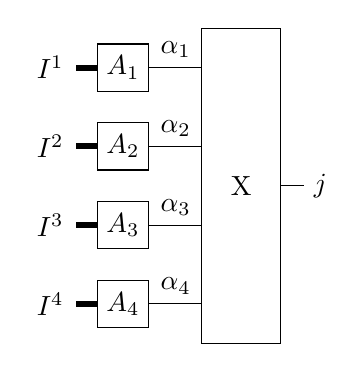
\begin{tikzpicture}[baseline=0.5]
        \draw (0,2.5)-- (0,-1.5) -- (1,-1.5)-- (1,2.5) -- cycle;

        \node[draw=none] (x)  at (0.5,0.5) {X};

        \node[draw, minimum size=0.6cm] (n1)  at (-1,2) {$A_1$};
        \node[draw, minimum size=0.6cm] (n2)  at (-1,1) {$A_2$};
        \node[draw, minimum size=0.6cm] (n3)  at (-1,0) {$A_3$};
        \node[draw, minimum size=0.6cm] (n4)  at (-1,-1) {$A_4$};

        \draw (n1) -- node [above] {$\alpha_1$} (0,2);
        \draw (n2) -- node [above] {$\alpha_2$} (0,1);
        \draw (n3) -- node [above] {$\alpha_3$} (0,0);
        \draw (n4) -- node [above] {$\alpha_4$} (0,-1);

        \draw[line width=0.75mm] (n1) -- ++(-0.6,0) node [left] {$I^1$};
        \draw[line width=0.75mm] (n2) -- ++(-0.6,0) node [left] {$I^2$};
        \draw[line width=0.75mm] (n3) -- ++(-0.6,0) node [left] {$I^3$};
        \draw[line width=0.75mm] (n4) -- ++(-0.6,0) node [left] {$I^4$};

        \draw (1,0.5) -- (1.3,0.5)  node [right] {$j$} ;

    \end{tikzpicture} }

\def \blockct { 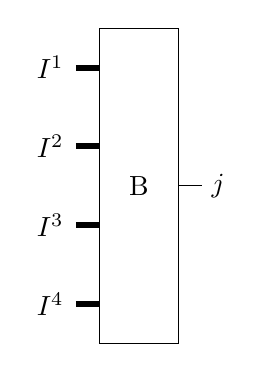
\begin{tikzpicture}[baseline=3]
        \draw (0,2.5)-- (0,-1.5) -- (1,-1.5)-- (1,2.5) -- cycle;

        \node[draw=none] (x)  at (0.5,0.5) {B};

        \draw[line width=0.75mm] (-0.3,2)  node [left] {$I^1$}  -- (0,2) ;
        \draw[line width=0.75mm] (-0.3,1)  node [left] {$I^2$} -- (0,1);
        \draw[line width=0.75mm] (-0.3,0)  node [left] {$I^3$} -- (0,0);
        \draw[line width=0.75mm] (-0.3,-1)  node [left] {$I^4$} -- (0,-1);

        \draw (1,0.5) -- (1.3,0.5)  node [right] {$j$} ;

    \end{tikzpicture} }

An exmple of this procedure is
\begin{align}
    \pepoat                    & = \blockat                        \\
    \pepobt                    & = \blockbt                        \\
    \vcenter{\hbox{ \pepoct }} & =  \vcenter{\hbox{  \blockct }} .
\end{align}
On the first line, the original problen is shown. The second line groups the physical indices in legs, and transforms the right-hand side accordingly. The third line shows the tensors in the form of \cref{axb}.

The most obvious way to solve this system is by using a linear solver. This results in some numerical problems. This is a result of the potentially ill conditioned inverses inherent to the construction. A pseudo-inverse of the full matrix can be easily obtained and resolves this issue (see for numerical example \cref{subsec:inversion_procedure}).

The pseudoinverse $A^{+}$ of matrix A is calculated as follows:
\begin{align}
    A     & = U \Sigma V^{\dagger}     \\
    A^{+} & = V \Sigma^{+} U^{\dagger}
\end{align}
Where for $\Sigma^{+}$ all the non-zero diagonal elements are replaced by their inverse. In the numerical pseudoinverse, every singular value below a given threshold e.g. $\sigma_0 = 10^{-12}$ is set to zero.

The problem with this full inverse is that the bond dimension increases very fast: matrix A has dimension $d^ {2 \sum_m n_m } \cross d^ {2 \sum_m n_m } $. Although using a linear solver instead of full inversion is considerably faster, this method still becomes infeasible for very quickly.

\subsubsection{Sequential inverse}

A second method consist of solving the following sequence of linear problems one leg at a time:

\begin{equation}
    \begin{split}
        A^1_{ I^1 \alpha^1 } X_{ \alpha^1  I^2 \cdots I^m j} &=  B_{  I_1  I_2 \cdots I_m   j }\\
        A^2_{ I^2 \alpha^2 } X_{ \alpha^1   \alpha^2  I^3 \cdots I^m j} &=  B_{  \alpha^1  I_2 \cdots I_m   j }\\
        &\vdots\\
        A^m_{ I^m \alpha^m } X_{ \alpha^1 \alpha^2 \cdots \alpha^m j  } &=  B_{ \alpha^1 \alpha^2 \cdots \alpha^{m-1} I_m   j }\\
    \end{split}
\end{equation}
While this method is very quick and scales well, in practice it results in unstable result. Solving sequentially, the errors of the pseudo-inverses (or worse full inverse) accumulate. If there are 4 legs, the threshold needs to be set at $ \sigma_0 = \sqrt[4]{ 10^{-12} } $. The inverse now becomes a bad approximation of the problem, rendering the results useless.

\subsubsection{Sparse full inverse}

Luckily the problem can be resolved by first performing an SVD decomposition of $A^m_{ I^m \alpha^m } = U^m_{ I_m \beta^m } S^m_{\beta^m \gamma^m}  V^{m\dagger}_{\gamma^m \alpha^m}$ matrices, with S diagonal and U and V unitary. All the $U^m$ matrices can be inverted by applying the Hermitian transpose to the leg m of B. The Tensor $S = S^1 \otimes S^2 \cdots \otimes S^m$ is very sparse and can be (pseudo)-inverted at once. For a full rank construction, $S$  is already diagonal. For truncated constructions (or inverses involving loops), this is no longer the case.
The last step consist of applying all the matrices $V^m$ to the right-hand side. This is shown in this equation
\begin{alignat}{1}
    A^1_{ I^1 \alpha^1 }   A^2_{ I^2 \alpha^2 }  \cdots  A^m_{ I^m \alpha^m }   X_{ \alpha^1  \alpha^2  \cdots \alpha^m j } & =  B_{  I_1  I_2 \cdots I_m   j }               \\%%%%%%%%%%%%%%%%%%
    U^1_{ I_1 \beta^1 } S^1_{\beta^1 \gamma^1}  V^{1\dagger}_{\gamma^1 \alpha^1}                                            & \nonumber                                       \\
    U^2_{ I_2 \beta^2 } S^2_{\beta^2 \gamma^2}  V^{2\dagger}_{\gamma^2 \alpha^2}                                            & \cdots  \nonumber                               \\
    U^m_{ I_m \beta^m } S^m_{\beta^m \gamma^m}  V^{m\dagger}_{\gamma^m \alpha^m}                                            & \nonumber                                       \\
    X_{ \alpha^1  \alpha^2  \cdots \alpha^m j }                                                                             & =  B_{  I_1  I_2 \cdots I_m   j }               \\ %%%%%%%%%%%%%%%%%%%%%%%%%%%%%%
    S_{ (\beta^1 \beta^2 \cdots \beta^m) (\gamma^1  \gamma^2 \cdots \gamma^m)  }                                            & \nonumber                                       \\
    V^{1\dagger}_{\gamma^1 \alpha^1}   V^{2\dagger}_{\gamma^2 \alpha^2}  \cdots  V^{m\dagger}_{\gamma^m \alpha^m}           & \nonumber                                       \\
    X_{ \alpha^1  \alpha^2  \cdots \alpha^m j }                                                                             & =  B'_{  \beta_1  \beta_2 \cdots \beta_m   j }.
\end{alignat}

The complexity is determined by the SVD decomposition of the individual legs. Due to its sparsity, S does not take much space to construct and is quite fast to pseudo-invert. Doing the pseudo-inverse at once means that it has the same precision as the full pseudo-inverse, as desired.

It is also possible to take a pseudoinverse of a matrix with a QR-decomposition, which is faster \cite{Moylan2016}. The Q could be inverted directly, and the $R = R^1 \otimes R^2 \cdots \otimes R^m$  matrix is still upper triangular. This method is not used because of the memory requirements to store this matrix is quite large.

\subsection{Extension}
The linear solver is made for problems linear problems. Nevertheless, it can solve every local patch appearing in a map, such as 2 neighbouring sites. These sites are split using an SVD decomposition. Another example is the following corner block, which can perfectly be solved with the linear solver.
\begin{equation}
    \pepob{5}{3}{{
                "-","-", "-",     "-",
                "-","1","$\beta$","-",
                "-","-","$\alpha$","-"}}{{
                "-","-",
                "-","-",
                "-","$\gamma$",
                "-","$\alpha$",
                "-","-"}}{{
                1,1,1,1,1,
                1,0,0,0,1,
                1,1,0,0,1}}
\end{equation}
The algorithm will treat this as 2 legs.

\subsection{Nonlinear solver}

In some cases, the above solver does not return the best possible solution to a given problem. The reason is that it is not able to incorporate symmetries or solve problems where the new blocks appear more than once. A new solver is needed which does not rely on methods from linear algebra, but on more general nonlinear least squares solvers.

In essence, the nonlinear least squares solver needs as input a vector with the error values $\vec{f}( \vec{x} )$, and if possible also the Jacobian, i.e. $ J_{I,J}  = \frac{ \partial f_I }{ \partial x_J } $. This info is used to choose a direction and a step size, minimising the error. An improved point x is chosen by the algorithm, until some convergence criterium is reached. The implementation uses MATLAB fsolve routine, which uses Levenberg-Marquardt algorithm under the hood.

\subsubsection{Automatic differentiation}
With some care, the Jacobian can be calculated for a general tensor network in an automated way. Suppose we want to differentiate the contracted tensor $T^{i_1  \cdots i_n  }$ with respect to one of the PEPO blocks $x_n = O^{i_n }_{\alpha \beta \gamma \delta}$. Denote $I=(i_1 \cdots i_n )$ and $J=(i_m  \alpha \beta \gamma \delta)$, and this block only occurs once. Then $  J_{I J}  = \frac{\partial T^{i_1  \cdots i_n  } }{  \partial O^{i_m }_{\alpha \beta \gamma \delta} } = T^{i_1 \cdots i_n } _{ i_m  \alpha \beta \gamma \delta}  \delta^{i_n}_{i_m}   $  amounts to  contracting the network with the tensor $x_m$ removed, and treating the non-contracted indices as external ones.

If a tensor appears in multiple places, the sum rule for derivatives has to be used.

\subsubsection{Symmetry}

The nonlinear solver can handle rotated and permuted blocks. For instance, a simple loop (square) can be solved by rotating one tensor $T^I_{ \alpha \alpha 0 0}$ 4 times, once for every corner. The Jacobian should be adapted according to the chain rule. Another example is the following decomposition:  $  X^I_\alpha X^J_\alpha = T^{I J} $, which is used in \cref{eq:rotsympepo}.

\subsubsection{Combining problems}
As only solver, the nonlinear solver can solve multiple (non-neighbouring) tensors at once, and do this for multiple maps at once.

\subsection{Sequential linear solver}
While from the previous section it seems all nonlinear problems need to be solved with the nonlinear solver, this is in fact not the case. This solver takes as input multiple new tensors, and solves them one by one. As this is not truly a linear system, the error will not be zero after one pass. But solving the tensors repeatedly lowers the error at each step, giving an iterative procedure. This procedure can be sped up by reusing some parts of the calculations involved in the linear solver. For example, the exponentiated Hamiltonian and contraction of all virtual levels that do not involve the optimised blocks only needs to be performed once.

The step is chosen as follows: suppose X is the current tensor and X' the newly computed one. Then the tensor is updated as follows: $X \leftarrow X + \alpha (X'-X)$. If the error has increased, the step is made smaller. The algorithm stops after a number of steps or when a certain threshold is reached.

\subsubsection{Conclusion}

The framework is equipped with 3 different solvers, designed to solve different problems. The code below shows how they are called from within the code:
\begin{verbatim}
[obj, ln_prefact, err] = solve_lin_and_assign(obj, map, {pattern}, 
                ln_prefact, struct);
[obj, ln_prefact, err] = solve_sequential_lin_and_assign(obj, map, {pattern},
                ln_prefact, struct, {rot_90});
[obj, ln_prefact, err] = solve_non_lin_and_assign(obj, {map}, {pattern}, 
                ln_prefact, struct, {rot_90});
\end{verbatim}
They only need a map, which is the geometry of the problem, and a pattern, i.e. the new block to add. \verb#rot_90# is an optional argument, listing all the permutations (such as rotation symmetry over 90 degrees). For completeness, \verb#ln_prefact# is the normalisation factor as discussed will be discussed in the next \cref{subsec:nf}.

Whenever the linear solver can be used, it is the solver of choice. The sparse full inverse procedure is fast and handles the ill-conditioned inverses very well. The sequential linear solver builds on this solver to handle the introduction of multiple new tensors, possibly related to each other through a permutation.

The nonlinear solver is at the moment only the fastest for small highly nonlinear problems, such as solving \cref{tikzfig:plaquetter} in a rotation invariant manner. The nonlinear solver can optimise multiple problems at once, and could be extended to fully use internal symmetries of the model.

\section{Optimisation}

\subsection{Bookkeeping}

One important aspect of programming these general solvers is to devise a scheme that keeps track of all the involved tensors and transforms to problem to the form described above. In the code, the geometric info is represented by a map. This keeps track of the neighbours for each site, numbers the internal and external legs and a list to perform the contractions.

The framework provides some tools to transform these maps into other maps, for instance by removing 1 site.

\subsection{Fast contraction}

One particular task is to determine all the possible combinations of virtual levels for a given geometry. Simply looping over all possible combinations scales as $n^m$, with the number of virtual levels and m the number of internal legs. This quickly becomes a bottleneck.
This problem can be restated as a PEPS contraction in the following way: for each site make a tensor $ T^{i}_{  \alpha \beta \gamma \delta } $ where i encodes all the non-empty combinations of legs $(\alpha \beta \gamma \delta)$. On each site, the right boundary conditions need to be applied to get the right geometry. After setting the boundary conditions, the sparse PEPS network can be contracted and the resulting tensor gives, after decoding, all the possible contractions. Due to its sparsity, this performs quite fast.
As an added bonus, removing a tensor from T gives all contractions without this tensor. As both results are sorted list, the subset of contractions containing a given tensor can also be found fast.

\subsection{Normalisation}\label{subsec:nf}

For many of the end results, the PEPO cells can be divided by a normalisation factor. Normalising the calculations is important, because $\exp( \hat{H})$ scales exponentially in the number of sites. Luckily, the exponential can be calculated directly in normalised form. Suppose H is the matrisation of the Hamiltonian evaluated for a certain geometry. This is a Hermitian matrix and can be diagonalised $H= Q D Q^{\dagger}$ with Q unitary. Then
\begin{align}
    exp(  H_{d^N} - N \alpha I  ) & =  Q exp(  D- N \log(\alpha ) I    ) Q^{\dagger} \\
                                  & =  Q \begin{bmatrix} exp(D_{1 1} - N \log(\alpha )) &        &                                     \\
                                               & \ddots &                                     \\
                                               &        & exp(D_{ d^N d^N} - N \log(\alpha )) \\
    \end{bmatrix}  Q^{\dagger}     \\
                                  & = \frac{  exp(  H_{d^N} ) }{ \alpha^N }.
\end{align}
With $I$ the unit matrix. Next to a global normalisation factor, every block calculation calculates a specific normalisation factor such that the largest eigenvalue of $exp(H)$ is of the order 1.

\subsection{Internal representation}

Two main internal representations are used to construct the given MPO. Either, the MPO is stored as a cell of matrices, or as one big matrix where the blocks are added to during the construction. The output type can be chosen. For some types, sparse matrices are used during the construction. Given that Matlab doesn't support multidimensional matrices by default, \href{https://nl.mathworks.com/matlabcentral/fileexchange/29832-n-dimensional-sparse-arrays}{this}\cite{Matt} library is used.

\subsection{Even faster inverses}

% \def \figoneb {\expH{2}{$A$}{{,}}{{,}}{{,}}}
% \def \figthreeb {\expH{3}{$B$}{{,,"$i_3$"}}{{,,"$j_3$"}}{{,"v"}}}
% \def \figtwob {\mpo{1}{{"w","v"}}{{"$i_3$",}}{{"$j_3$",}}{} {}}
% \def \figfour { \expH{1}{$A^{-1}B$}{{"$i_3$",}}{{"$j_3$",}}{{"u","v"}} }

% \begin{equation}
%     \begin{split}
%         \combineTikz{ \figoneb }{\figtwob}{1.8} &=  \figthreeb \\
%         \figtwob &= \figfour
%     \end{split}
%     \label{eq_mpoinvdef}
% \end{equation}

While the inversion procedure above states how to make use of pseudoinverses, it was not yet clear in the 1D case it was needed. The 1D implementation uses a trick to get all the inverses for free from the SVD decomposition. Take the MPO which corresponds to a unitary matrix:

% \def \figone {\expH{2}{$O^{u v,v w}$}{{"$i_1$","$i_2$"}}{{"$j_1$","$j_1$"}}{{"u","w"}}}

% \begin{equation}
%     \figone  = \mpo{2}{{"u","v","w"}}{{"$i_1$","$i_2$"}}{{"$j_1$","$j_1$"}}{}{}
% \end{equation}

% \begin{equation}
%     \begin{split}
%         U^n_{(\alpha i j) \beta} & A_{\beta \gamma} = B_{\alpha i j \gamma} \\
%         &A_{\delta \gamma} =   U^{ n\dagger}_{\delta (\alpha i j)} B_{\alpha i j \gamma}
%     \end{split}
% \end{equation}
% If we now define the MPO $O^{-1}_n$ equal to $U^{n \dagger}$ with the second index split and permuted:

\begin{equation}
    \mpo{1}{ {"$\delta$","$\beta$",}  }{ { "$i$",}}{ { "$j$",}}{}{ {"$O_n$",} } \cong U^{n}_{\alpha (i j \beta)}
\end{equation}
Then the inverse MPO can be calculated by taking its Hermitian conjugate and reshaping.
\begin{equation}
    \mpo{1}{ {"$\beta$","$\gamma$",}  }{ { "$i$",}}{ { "$j$",}}{}{ {"$O^{-1}_n$",} } \cong U^{n \dagger}_{ (i j \beta)  \gamma }
\end{equation}
% With the notation from \cref{eq_mpoinvdef} we have:
% \def \OnBlock {\expH{4}{ $L_n^{-1} $  }{ {,,"...",} }{ {,,"...",} }{{"$\alpha$",0}} }
The left inverse looks like
\begin{equation}
    2 =  \mpo{4}{ {"$\alpha$",,,,0}  }{ {,,,,,}}{ { ,,,,,}}{{0,0,1,0}}{{"$O^{-1}_n$","$O^{-1}_m$",,"$O^{-1}_1$",} }
\end{equation}
where the physical indices need to be contracted with the corresponding indices of the right-hand side.

\subsection{Buffering Results}

Some calculations, such as calculating the matrix exponential, take some time. In 1D code, the same calculations were performed over and over again, and hence a buffer mechanism was written to store these results. In the 2D framework, this not necessary as the solvers only calculate the matrix exponential once and return the blocks together with the made error.

\subsection{Profiling}
To get a sense of the speed, constructing a 2D PEPO up till order 6 with level 3 truncated at bond dimension 20 with loop extensions takes about 25 seconds on my pc. The most time intensive processes are performing the contractions. For larger systems, the time limiting factor is calculating the exponential of the Hamiltonian.

\subsection{Calculating the error}

Every solver returns the residual error for the new block. This comes at almost no cost, because all the calculations are already done during the solving procedure.

\section{Calculating phase diagrams} \label{sec:phase_diag}

This section details how the phase diagrams are calculated, stored and the critical parameters fitted. The results are discussed in \cref{subsec:2dpahsediag}.

\subsection{Points sampling}

This concerns the problem which temperatures to select to calculate the phase diagram. As  the transition between 2 phases is sharp, a uniform sampling in T is not the best option. A very fine grid is needed to capture the transition well, requiring high computation times.
The sampling starts by calculating the magnetisation for N  uniformly sample points between 2 temperatures. These calculations are performed in parallel on a multicore server. When they are all finished (or have run for a maximum amount of iterations), all the arch lengths are calculated, and repeatedly a new T point is inserted in the largest interval until N new points are selected. The arch length in the m-T plan can be changed to require more points in the m direction than T direction.

\subsection{Storing the information}

Each run has a template with all the common model info. For each point 2 files are stored. One file contains the info and results, such as temperature, magnetisation, correlation length, etc. The other file is much larger and contains the PEPO tensor, the calculated VUMPS environments, \dots
The files of the first kind are used in other calculations, such as fitting procedure.  Reassembling the files into one structure happens in a central function. Another function is able to reprocess already calculated points. The sampling can be continued from where it was last stopped.

\subsection{Fitting}\label{subsec:qphasediag}

The coded performs a finite-size scaling as explained in \cref{subsec:fss}.

The fitting procedure works as follows: a function $f_X$ defined by a limited number of parameters is made for every observable $X \in \{ m , \xi, S \}$. The parametrisation is chosen such that it has the right scaling behaviour, and the analytical derivative is known.

The code performs a nonlinear optimisation, where the error is either the vertical distance to $f_X$ or the orthogonal distance. The fitted function and parameters are determined simultaneously.

The optimisation runs for a limited number of cycles. Afterwards, a random displacement is made to the parameters of the current best fit. This is repeated until convergence.

The code to perform this collapse was originally written by Bram Vanhecke and adapted to its current form. This includes the possibility to fit he subleading corrections and $c_i$ to calculate $\delta$.

\section{How to use}\label{sec:H5:source_code}

All the code neede to generate all the results from this dissertation is available on my github page \url{https://github.com/DavidDevoogdt/Thesis_Tensor_Networks}. The starting points to explore the code are in the readme file.

\subsection{Source code structure 1D}

The source code for this project can be found on \href{https://github.com/DavidDevoogdt/Thesis_Tensor_Networks}{github}. The implementation of these types can be found under \path{src/generateMPO.m}. In this class the different types of MPO can be constructed. It bundles some helper functions such as contracting a chain or cycle of MPO's or construction of an exponentiated hamiltonian for the given input hamiltonian. Other examples are making $L_n^{-1}$ by sequential invers MPO contractions,...

\path{src/test.m}  contains the code to create the plots to compare different types and orders. The other files in the folder are self-explanatory.

\subsection{Source code structure 2D}

\todo{source code 2D}


\section{Limitations and outlook}

In short, all components are in place in the framework to generate easily and efficiently all the blocks.

\subsection{Implementation}

By far the largest amount of time invested in this thesis was creating and testing this framework. Everything (except the fitting code) was written from scratch. Implementation of the maps and solvers in its full generality is a very error-prone problem. In hindsight, the 1D framework may seem unneeded, given that the 2D framework is even better. This is not the case. Constructing the 2D framework was only possible due to the lessons learned (and mistakes made) in the 1D code.

\subsection*{Code quality}
The first and most important goal of writing numerical code is of course that it compiles and that the results are as correct. But this is only the first step. The 2D framework neatly orders the different task is functions to avoid as much code duplication as possible. This improves readability and decreases the number of errors as every component is used in many ways.

\subsection*{Size limitation}
The main bottleneck is, as expected, calculating the matrix exponential for large systems (N>14). For large maps, contracting the PEPO network is an equally expensive operation. The other components are efficient enough to not cause any troubles. In particular, the solvers aren't a limiting factor at this point to go further.

\subsection*{Lattices}
The models studied were all on a square lattice. It would be beneficial to be able to simulate other lattices, but also higher dimensions could be included. In essence all the information of the lattice is contained in the maps generated for each calculation, such as all the connected sites, how to contract them, etc. Although undoubtedly many details will need to be changed to use it in practice, the solvers can stay almost the same.

\subsection*{Symmetries}

At the moment rotation and permutation symmetries can be included in the construction of the blocks. Internal symmetries are not yet included. This could push computational boundaries further.


\chapter{Results} \label{chap:results}

\epigraph{With four parameters I can fit an elephant, and with five I can make him wiggle his trunk}{John von Neumann}

%\section{Benchmarking}
%\subsection{dioganalsation}

The performance of the MPO construction can be compared with the exact diagonalisation of the hamiltonian for a given number of sites. To obtain a faithful results, the number of sites should be as high as possible. In practice, diagonalisation of large matrices becomes slow and memory consuming. The size grows exponentially in the number of sites: $d^{n} \times d^{n} $. A double takes 8 bytes of memory.A Rough estimated of the amount of RAM $R$ needed to store this complex array is:

\begin{equation}
    R = d^{2 n} \times 16 bytes
\end{equation}

Which means a 14 site chain already takes up  GB of RAM.

\todo{time complexity algoritms}

\todo{open chain or cyclical}


\subsubsection{norms}

\todo{trace norm, schatten p norm, ...}

The schatten 2 norm is used in the following analysis, dentoted by ${\| \cdot \|} _{2}$. In the figures the relative error $\epsilon$ is reported.


\def \expHBlock {\expH{4}{ $e^{- \beta \hat{H}_{n}}$   }{ {,,"...",} }{ {,,"...",} }{}{} }
\def \Mn {\mpo{4}{ {0,,,,0}  }{}{}{{0,0,1,0,0}}{}}


\begin{equation}
    \epsilon = \frac{  {  \left \|  \expHBlock - \Mn  \right \|} _{2}  }{ {  \left\|  \expHBlock \right \|}_2}
\end{equation}


\subsubsection{Ising}

The first model used to benchmark the different types of MPO's is the transversal ising model. For type A the $\epsilon$ increases with
$\beta$. As expected, the relative error decreases with increasing order.

The behaviour of type B is more chaotic. The error increases no longer monotonously. For small values of $\beta$, the order is truncated.


\begin{figure}[H]
    \center
    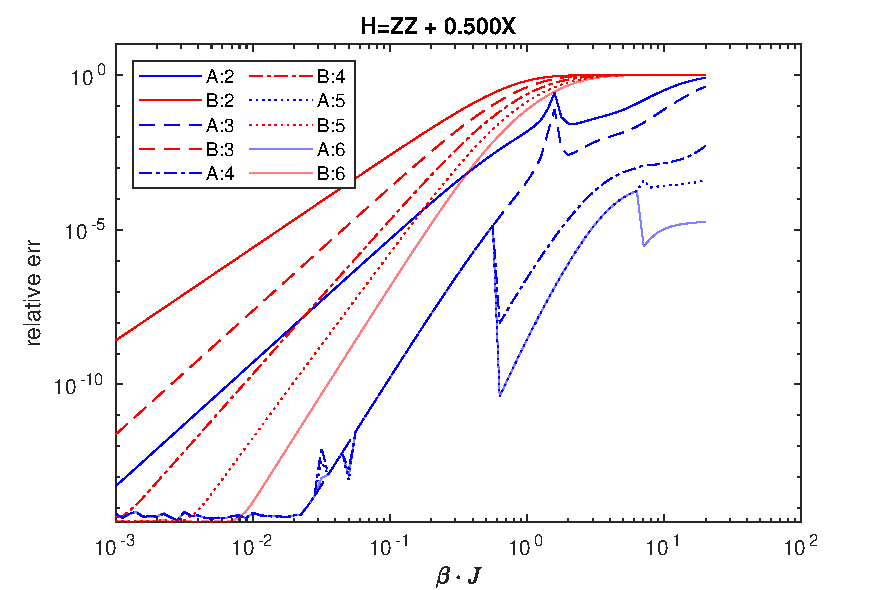
\includegraphics[width=\textwidth]{Figuren/benchmarking/t_ising_copmAB6.pdf}
    \caption{Comparison type A and B for Transversal Ising}
    \label{fig:benchmark:tising}
\end{figure}

\subsubsection{Heisenberg}

For the Heisenberg model, type A is also an improvement over type B. For large values of $\beta$, type A is not able to reproduce the exact


\begin{figure}[H]
    \center
    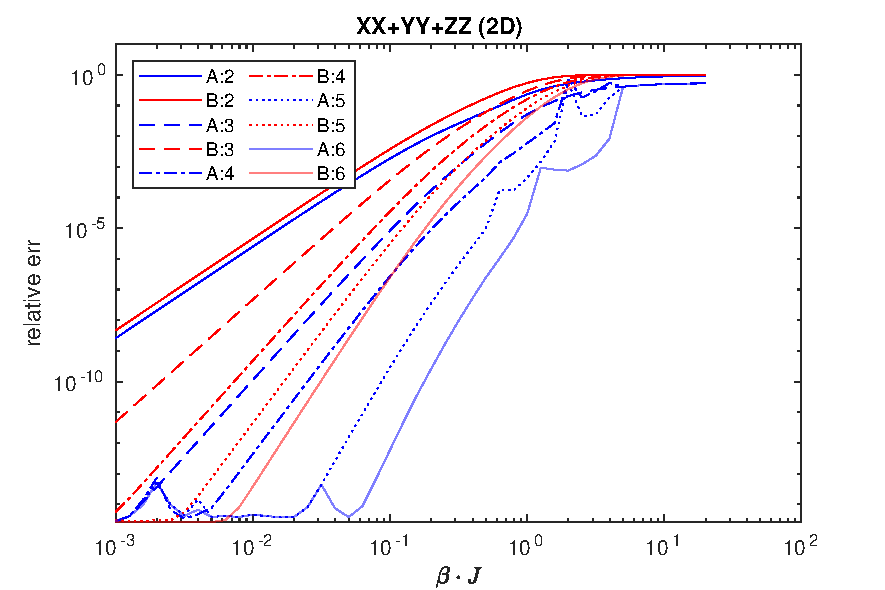
\includegraphics[width=\textwidth]{Figuren/benchmarking/heisenberg_compAB6.pdf}
    \caption{Comparison type A and B for Heisenberg}
    \label{fig:benchmark:Heisenberg}
\end{figure}


\todo{run with M=11}

\subsection{Random}

To give a representative overview for random hamiltonians, several simulations were run. The single site and nearest neighbourgh hamiltonians are generated by making hermitian matrices with random real and complex numbers between -1 and 1. In order to compare the different graphs, the engergy scale is set such that the norm of the 2 site hamiltonian is 1.


Clearly, the performance of type B is almost independent on the chosen random variables. For type A there is more variation. Sometimes there are spikes for a given $\beta$. Despite the worse relative error, higher orders (with exact the same lower order blocks) seem to remove the spike.

For most of the trials, orders higher than 6 get truncated.

\begin{figure}[H]
    \begin{subfigure}[]{\textwidth}
        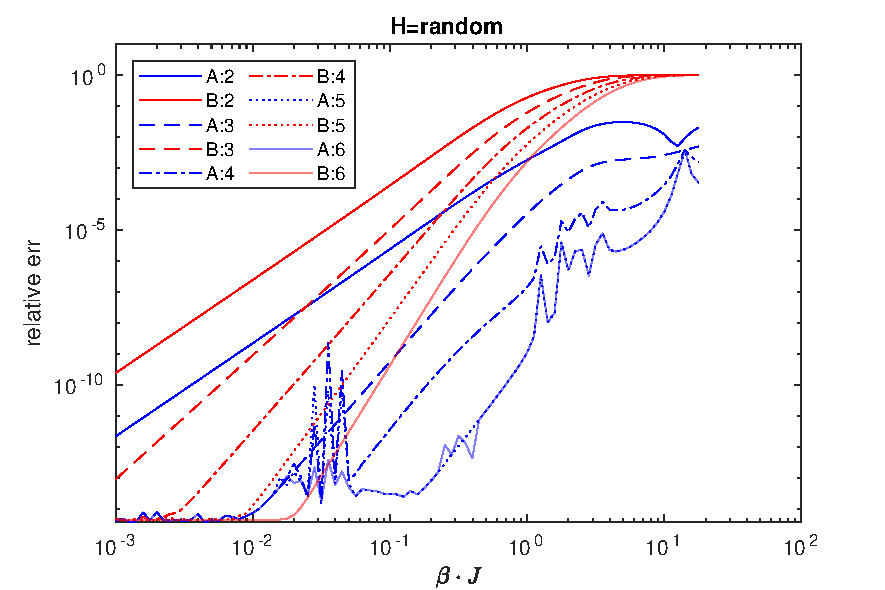
\includegraphics[width=\textwidth]{Figuren/benchmarking/random_copmAB6.pdf}
        \subcaption{test}
    \end{subfigure}

    \medskip

    \begin{subfigure}[]{\textwidth}
        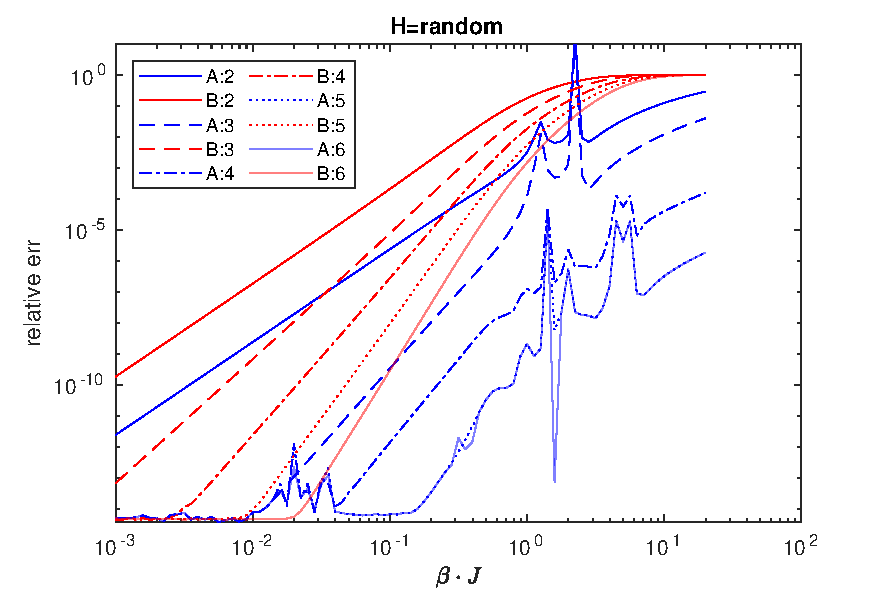
\includegraphics[width=\textwidth]{Figuren/benchmarking/random_copmAB6_2.pdf}
        \subcaption{test}
    \end{subfigure}

    \caption{test }
\end{figure}

\begin{figure}[H]\ContinuedFloat
    \begin{subfigure}[]{\textwidth}
        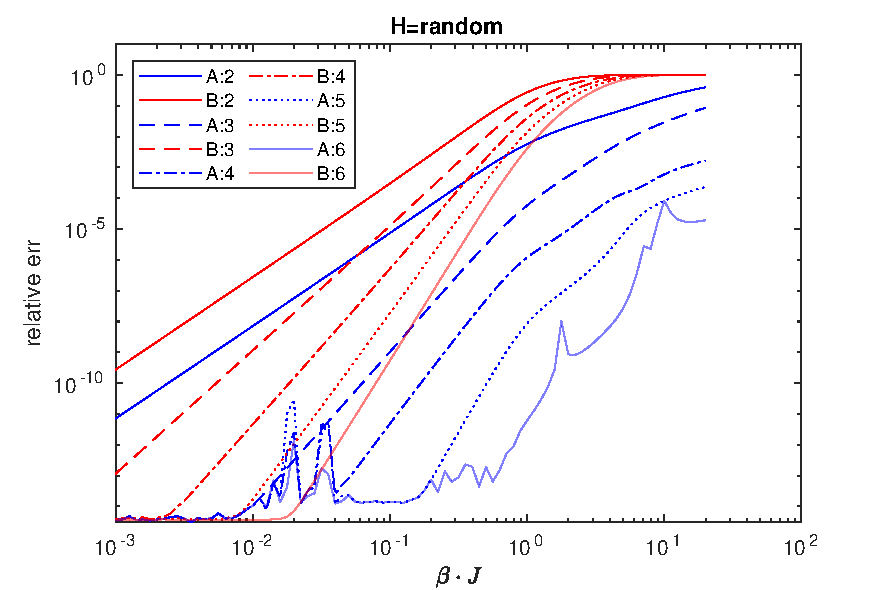
\includegraphics[width=\textwidth]{Figuren/benchmarking/random_copmAB6_3.pdf}
        \subcaption{test}
    \end{subfigure}

    \begin{subfigure}[]{\textwidth}
        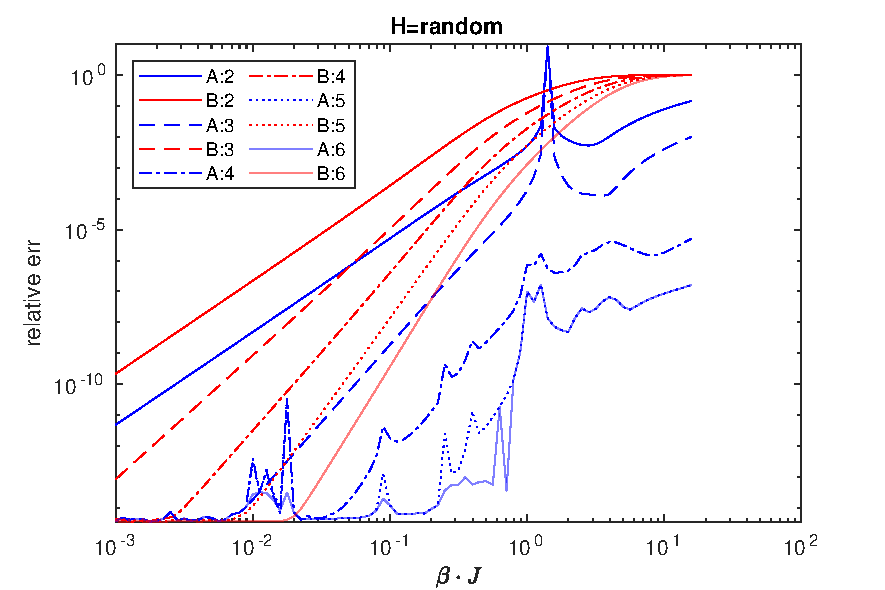
\includegraphics[width=\textwidth]{Figuren/benchmarking/random_copmAB6_4.pdf}
        \subcaption{test}
    \end{subfigure}
    \caption{test (cont.) }
    \label{fig:benchmark:Random}
\end{figure}


\subsection{analytical results}

\section{Introduction}
This section explains the acuracy and performance of the given cluster expansions. The first section compares the different constructions in 1D based on the error relative to the exact solution. The best algorithm will form the basis for the 2D results. First, similarly to 1D, the results will be checked based on the error relative to the exact solution. Then, the expansion is used to calculate the phase diagram of the 2D transversal field Ising model.

\section{Results 1D}\label{sec:results1d}
In this section the results of the MPO construction detailed in

\subsection{Exact tensor matrix exponential } \label{chap_bench}

The performance of the MPO construction can be compared with the exact diagonalisation of the hamiltonian for a given number of sites. To obtain a faithful results, the number of sites should be as high as possible. In practice, diagonalisation of large matrices becomes slow and memory consuming. The size grows exponentially in the number of sites: $d^{n} \times d^{n} $. A double takes 8 bytes of memory.A Rough estimated of the amount of RAM $R$ needed to store this complex array is:

\begin{equation}
    R = d^{2 n} \times 16 bytes
\end{equation}

Which means a 14 site chain already takes up more than 4 GB of RAM. The complexity to calculate a matrix exponential scales as $O(n^3)$ \cite{Moler2003}. In practice this means that, without any tricks, the matrix exponential can be calculated for 12 sites.

State of the art algorithm for exact diagonalisation, which include all symmetries and are optimised for parallelisation, can calculate up to 50 sites. \cite{Wietek2018}

\subsubsection{Norms} \label{mponormdef}
\def \expHBlock {\expH{4}{ $e^{- \beta \hat{H}_{n}}$   }{ {,,"...",} }{ {,,"...",} }{}{} }
\def \Mn {\mpo{4}{ {0,,,,0}  }{}{}{{0,0,1,0,0}}{}}

The schatten 2 norm is used in the following analysis, denoted by ${\| \cdot \|} _{2}$. In the figures the relative error $\epsilon$ is reported.

\begin{equation}
    \epsilon = \frac{  {  \left \|  \expHBlock - \Mn  \right \|} _{2}  }{ {  \left\|  \expHBlock \right \|}_2}
\end{equation}

This norm can only be calculated for a finite number of sites. The influence of the number of sites for a linear  and cyclic \cref{benchmarking:systemsize}. As expected, the cyclic norm represents large systems better for the same number of sites. The linear norm keeps increasing with every added site.

Calculating the cyclic norm comes at the extra cost of contracting a cyclic tensor network. In this chapter, the cyclic norm will be given for M=11 sites.

\begin{figure}
    \begin{subfigure}[]{\linewidth}
        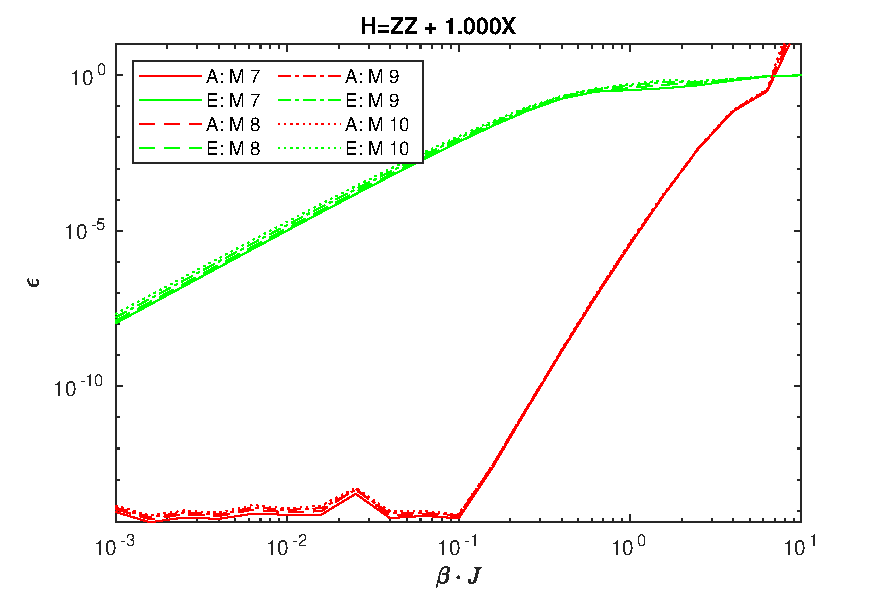
\includegraphics[width=\textwidth]{Figuren/benchmarking/comp_M_cycl.pdf}
        \subcaption{Cyclic error}
    \end{subfigure}
    \begin{subfigure}[]{\linewidth}
        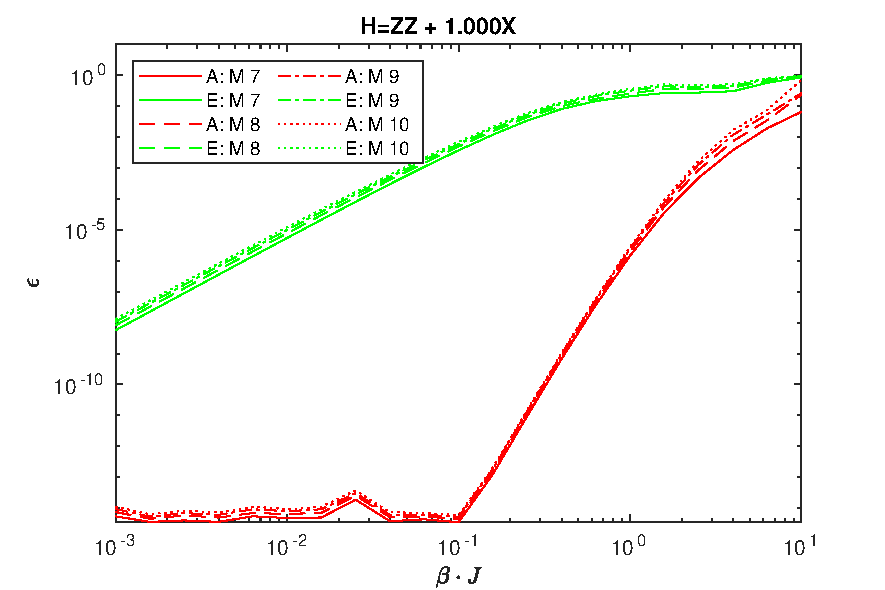
\includegraphics[width=\textwidth]{Figuren/benchmarking/Comp_M_lin.pdf}
        \subcaption{Linear error}
    \end{subfigure}
    \caption{ Different error measures for 1D transversal Ising model }
    \label{benchmarking:systemsize}
\end{figure}

\subsection{Inversion procedure}\label{subsec:inversion_procedure}

\subsubsection{Full pseudo-inversion}

The procedure for inversion of the linear blocks was detailed in \cref{subsec:linear_solver}. To demonstrate the need for a pseudoinverse, the error for transversal Ising models is shown in \cref{benc:fig:fullinv}. The pseudoinversion has 1 parameter $\sigma_0$, the cutoff below which the singular values are set to zero. A value of $10^{-12}$ seems optimal in the sense that it doesn't introduce large fluctuations, but still is able to produce good inverses.

\begin{figure}
    \center
    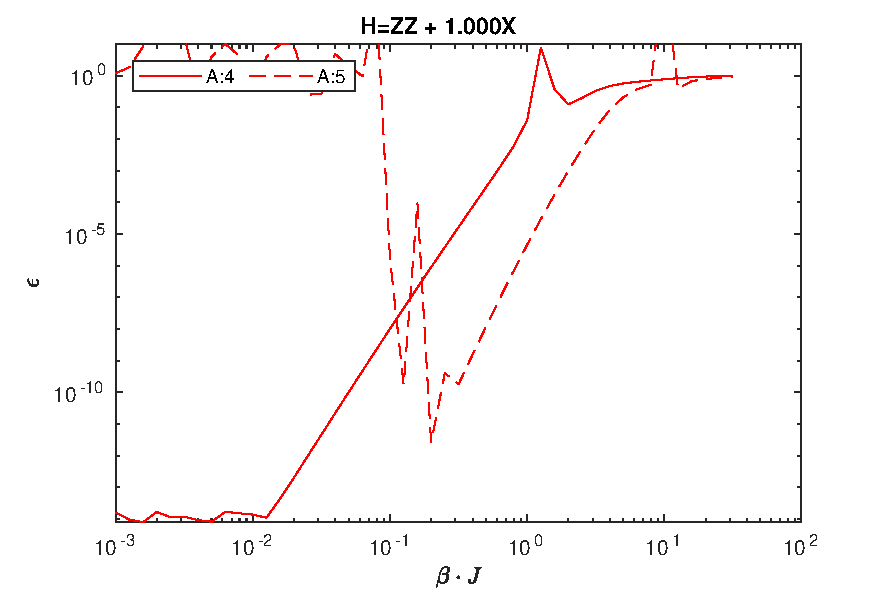
\includegraphics[width=\textwidth]{Figuren/benchmarking/t_ising_full_inverse.pdf }
    \caption{Error for transversal Ising, computed with full inversion }
    \label{benc:fig:fullinv}
\end{figure}

\paragraph{Truncation}

The original 1D code does not yet have this full inversion procedure. Instead, an optimality criterium was devised to truncate the series. Needless to say, even with this criterium, the results were a lot worse at low beta.

\subsection{Models}

With these basic definitions and findings out of the way, the different series expansions can be tested against some different physical models.

\subsubsection{Ising}

The results for the different types are all bundled in \cref{fig:benchmark:tising}. The vertical axis show the logarithm of the relative error $\epsilon$, horizontal axis the normalised inverse $beta= \frac{J}{T}$. The most surprising finding is the fact that the strict type E performs worse than the others. For low $\beta$, it is more than 5 orders of magnitude worse, Taken together with its large bond dimension, this expansion  and all other strict variants are seen to be of no use.

Now lets focus on the 2 other variants. Type A clearly outperforms type F for all $\beta<2$ by quite some margin. Only for large $\beta$, type F has the upper hand. While not completely clear in the picture, type A has quite a large error for some orders at $\beta \in (2,10) $, but higher orders seems to solve the problem. The construction of type F requires twice the bond dimension, and hence type A performs clearly better overal

\begin{figure}
    \center
    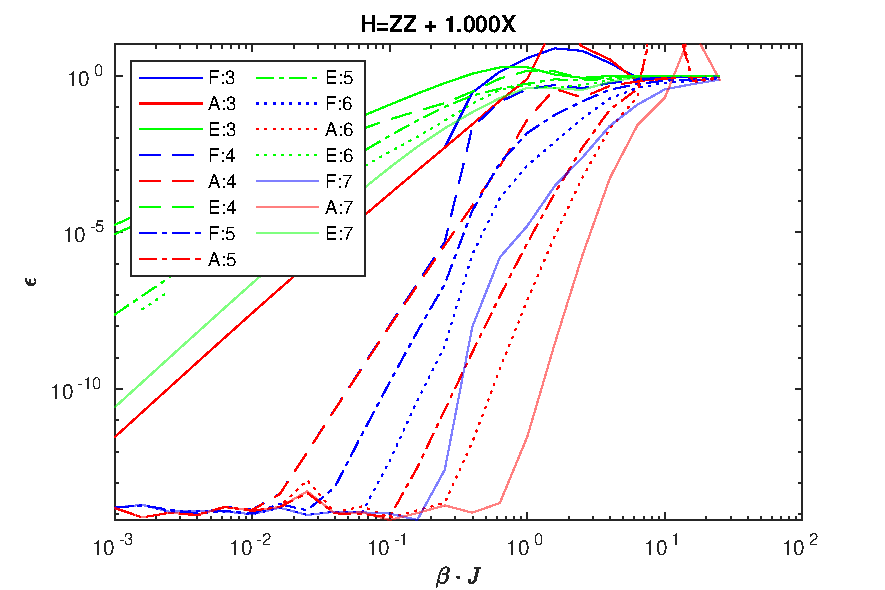
\includegraphics[width=\textwidth]{Figuren/benchmarking/t_ising.pdf}
    \caption{Comparison type A, E and F for Transversal Ising. }
    \label{fig:benchmark:tising}
\end{figure}

\subsubsection{Heisenberg}

Now we focus on the spin 1/2 Heisenberg model on a chain. The results are again displayed in \cref{fig:benchmark:tHeisenberg}. The exact type seems to perform a lot better here, but still has consistently the largest error of the 3 methods for a given order. For low $\beta$, type A again performs better than type F. At $\beta \approx 1$ and larger, F starts to improve upon the result of A, and doesn't have an divergent error.

\begin{figure}
    \center
    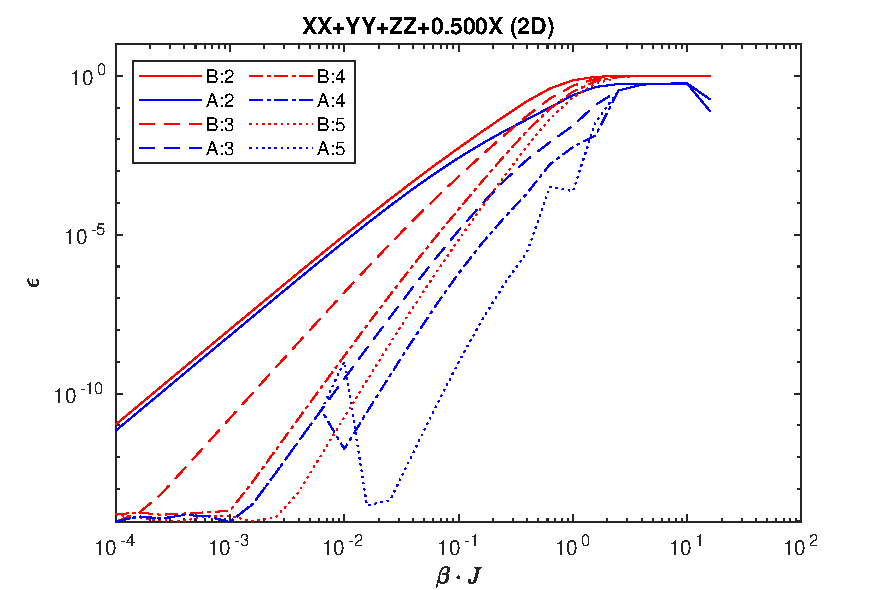
\includegraphics[width=\textwidth]{Figuren/benchmarking/t_heis_XXX.pdf}
    \caption{Comparison type A, E and F for Heisenberg model.}
    \label{fig:benchmark:tHeisenberg}
\end{figure}

\subsubsection{Random}

To give a representative overview for random hamiltonians, several simulations were run. The single site and nearest neighbour hamiltonians are generated by making hermitian matrices with random real and complex numbers between -1 and 1. In order to compare the different graphs, the energy scale is set such that the norm of the hamiltonian evaluated on 2 sites is 1.

\cref{fig:benchmark:trand} shows the results for 2 random hamiltonians. This is done to ensure that the chosen models are not too 'simple'. The results show once again that the strict variant performs worse than the other 2. In comparison to the previous models, Type F performs very well, especially at high $\beta$.

\begin{figure}
    \begin{subfigure}[]{\textwidth}
        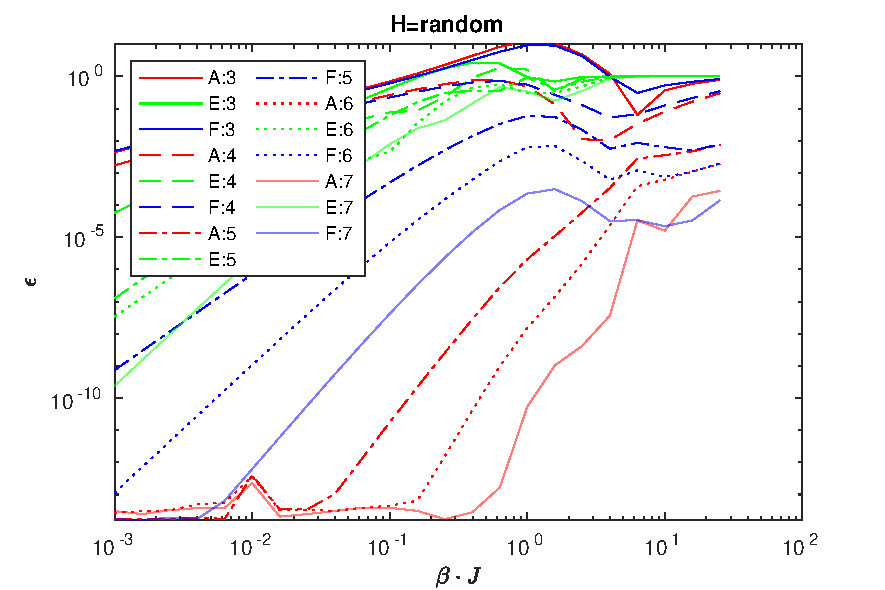
\includegraphics[width=\textwidth]{Figuren/benchmarking/1D_Raand.pdf}
        \subcaption{}
    \end{subfigure}

    \begin{subfigure}[]{\textwidth}
        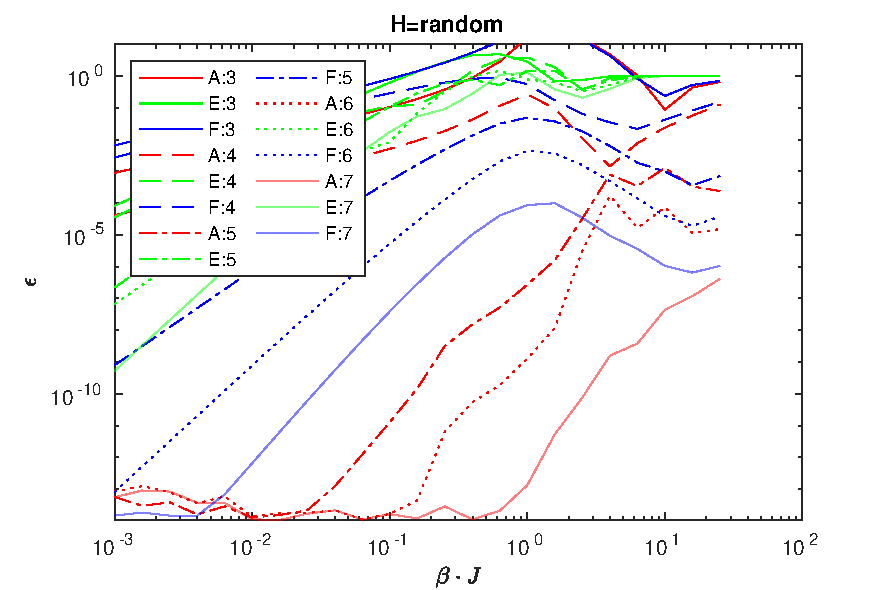
\includegraphics[width=\textwidth]{Figuren/benchmarking/1D_Raand_2.pdf}
        \subcaption{}
    \end{subfigure}

    \caption{Comparison type A, E and F for 2 random generated hamiltonians.}
    \label{fig:benchmark:trand}
\end{figure}

% \begin{figure}
%     \begin{subfigure}[]{\textwidth}
%         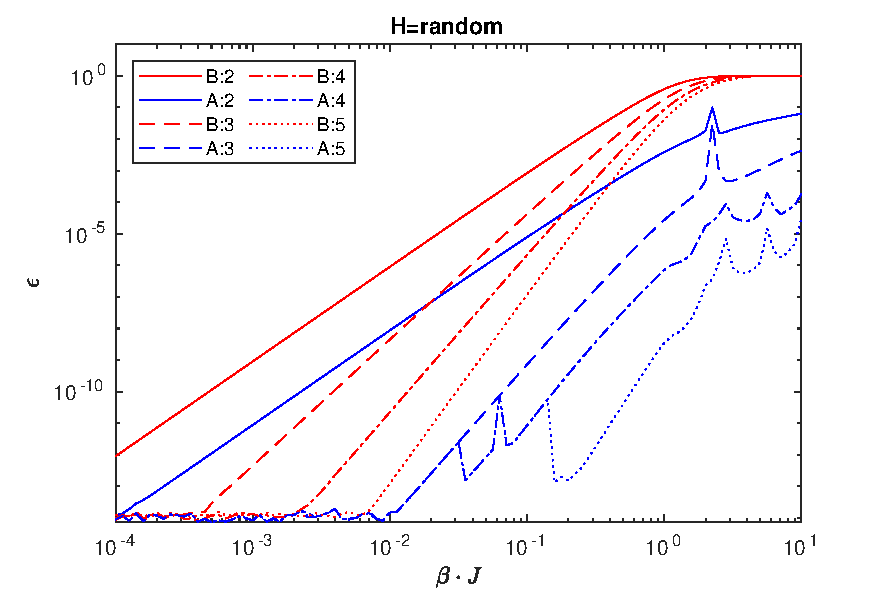
\includegraphics[width=\textwidth]{Figuren/benchmarking/rand_01.pdf}
%         \subcaption{test}
%     \end{subfigure}

%     \medskip

%     \begin{subfigure}[]{\textwidth}
%         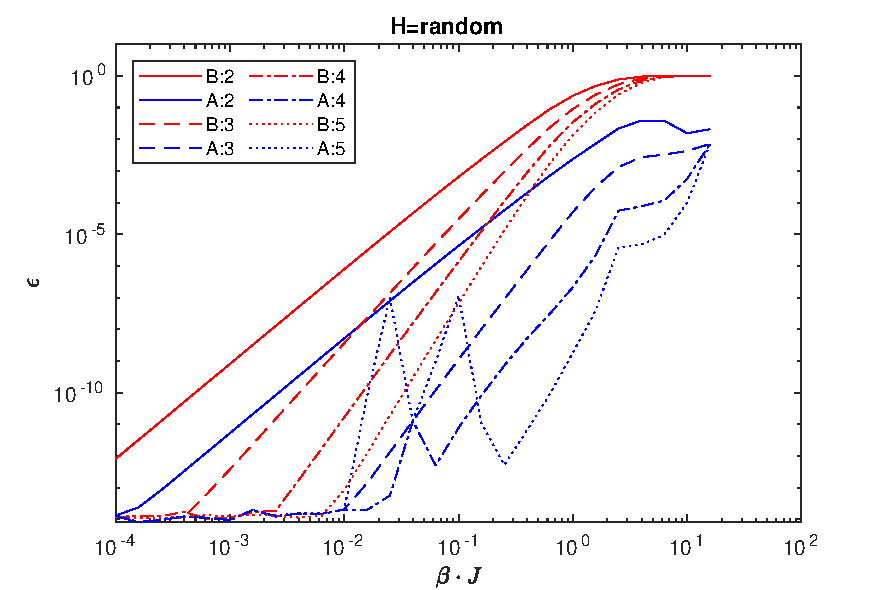
\includegraphics[width=\textwidth]{Figuren/benchmarking/rand_02.pdf}
%         \subcaption{test}
%         \label{benchmark:rand2}
%     \end{subfigure}

%     \caption{test }
% \end{figure}

% \begin{figure}[H]\ContinuedFloat
%     \begin{subfigure}[]{\textwidth}
%         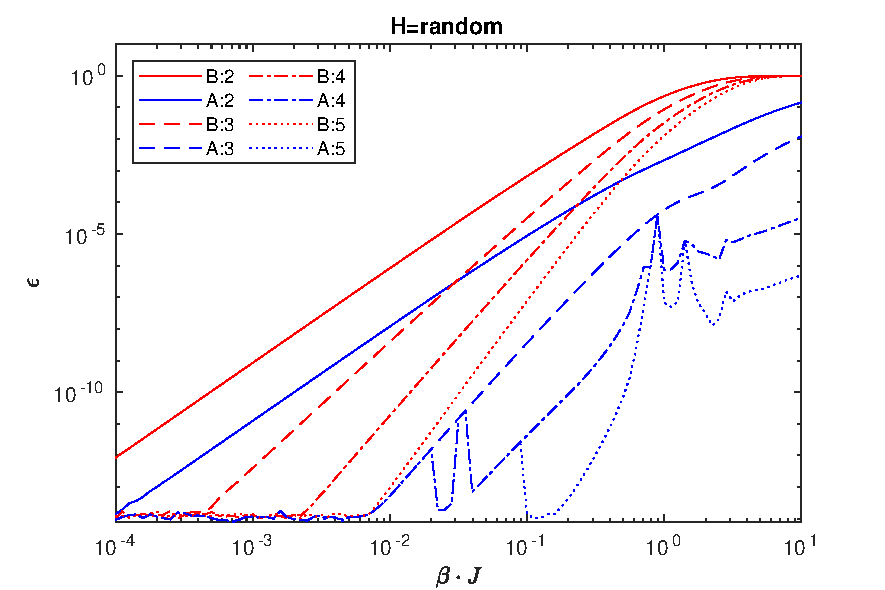
\includegraphics[width=\textwidth]{Figuren/benchmarking/rand_03.pdf}
%         \subcaption{test}
%     \end{subfigure}

%     \begin{subfigure}[]{\textwidth}
%         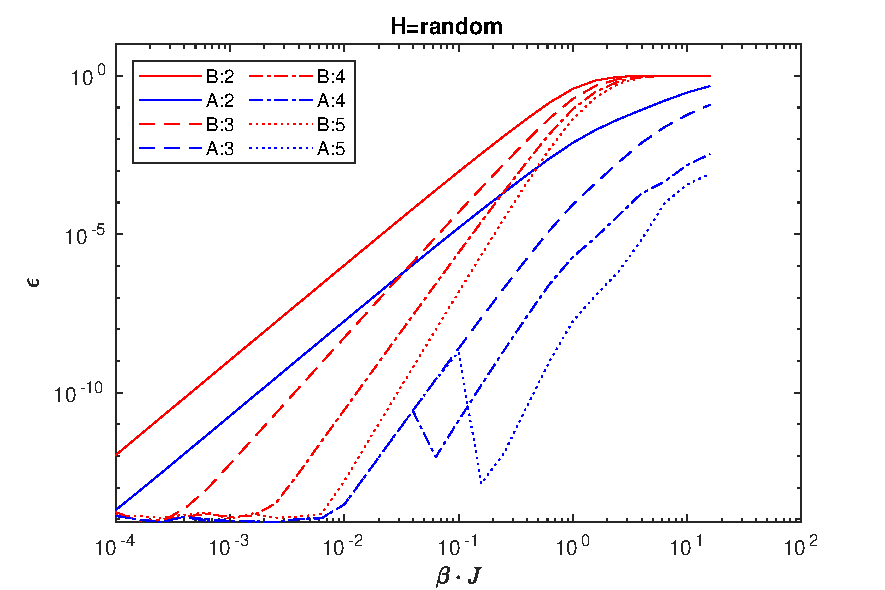
\includegraphics[width=\textwidth]{Figuren/benchmarking/rand_04.pdf}
%         \subcaption{test}
%     \end{subfigure}
%     \caption{test (cont.) }
%     \label{fig:benchmark:Random}
% \end{figure}

\subsection{Real time evolution} \label{subsec_rt_evo}

The method can also be used to construct real time evolution. \Cref{fig:benchmark:tising_time} shows the error of the matrix exponential in function of the time step $t = -i \beta $.

Also here, the results are promising. The construction handles complex matrices well. Similar to previous conclusion, type A performs better than type F, which performs better than type E.

The error of type A becomes quite large for high temperatures (not visible on figure), while type F keeps the errors low.

\begin{figure}
    \center
    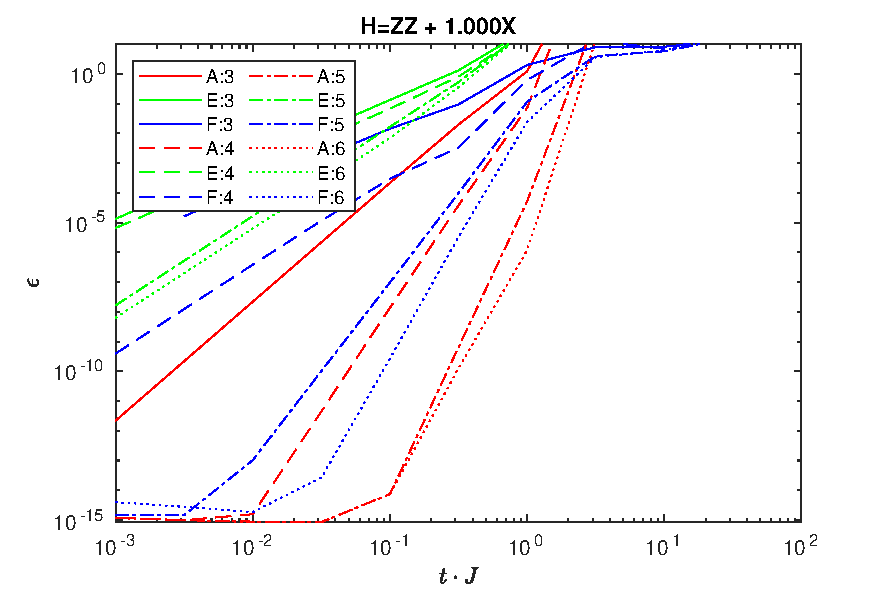
\includegraphics[width=\textwidth]{Figuren/benchmarking/1D_t_ising_time.pdf}
    \caption{Comparison type A, E and F for transversal Ising model. The horizontal axis represents the time step, not the inverse temperature. Virtual level 3 is truncated to $\chi=20$.  }
    \label{fig:benchmark:tising_time}
\end{figure}

This is not by any means a complete analysis of the real time evolution operator, but just a numeric example.

\subsection{Conclusion}

The biggest lesson, which took some time to figure out, was the correct way to implement the inversion procedure. It is essential that the pseudoinverse is taken for all the legs at once.
The different types were tested against each other, and it is clear that type A is clear that type A is better in almost all situations. The strict variants score worse. Type F keeps the inverses well-defined, and this shows at large $\beta$. Also, real time evolution works well.
The truncation procedure works as expected. A longer chain should not be constructed when a shorter chain was not solved fully (e.g. due to a truncation of the previous level)
Constructions with explicit rotation symmetry (see \cref{sec:symm}) perform exactly as good as the ones without.

\section{Results 2D}\label{sec:results2d}
The results in 1D are very promising, but the real open challenges are situated in 2 (or higher) dimensions. Therefore, it is an interesting and relevant question whether the results generalise to 2D. These results are twofold. On the one hand, a similar measure as in 1D is calculated to measure how good a method works on a specific 2D grid. Here, we will need to settle for what can be computed. As a second measure, and from physical point of view the most interesting one, some phase transitions of the 2D \Gls{TFI} model are determined, and compared against values in literature.

\subsection{Norm}

Once again, a suitable norm has to be derived. The situation is more difficult than in 1D, because contracting a PEPO \Gls{TN} has a much larger computational complexity than in 1D. Ideally, the norm would be calculated on an n by n cyclical grid (2D grid on a torus). Here n has to be at least 1 larger than the largest explicitly constructed chain. In practice, this is not achievable in a reasonable amount of time. The limitations are twofold: the maximum number of sites to calculate the matrix exponential is still around 14, and the contraction of the \Gls{TN} on a torus is limited to 3 by 3. This not capture the long chains.  The limitations on the PEPO contraction can be somewhat relaxed by not computing the full network, but computing the reduced density matrix. Here, most of the sites have their physical indices traced out, except for one site.

The final error measures are defined by:
\begin{equation}\label{res2d:err_Def}
    \rho^1_{i,j} =\vcenter{ \hbox{ \pepob{8}{8}{{
                        "-","-", "-","-","-","-","-",
                        "",  "", "","","","","",
                        "",  "", "","","","","",
                        "",  "", "","","","","",
                        "",  "", "","","","","",
                        "",  "", "","","","","",
                        "",  "", "","","","","",
                        "-", "-", "-","-","-","-","",}}{{
                        "-","-", "-","-","-","-","-",
                        "","", "","","","","",
                        "","", "","","","","",
                        "","", "","","","","",
                        "","", "","","","","",
                        "","", "","","","","",
                        "","", "","","","","",
                        "-","-", "-","-","-","-","",}}{{
                        1,13,1,1,1,1,1,1,
                        1,0,1,1,1,1,1,1,
                        1,0,1,1,1,1,1,1,
                        1,0,1,1,1,1,1,1,
                        1,0,1,1,1,1,1,1,
                        1,0,0,0,1,1,1,1,
                        13,12,0,0,0,0,0,13,
                        1,13,1,1,1,1,1,1,
                    }} }}
\end{equation}
and
\begin{equation}\label{res2d:err_Def_2}
    \rho^2_{i,j} =\vcenter{ \hbox{ \pepob{8}{8}{{
                        "-","-", "-","-","-","-","-",
                        "",  "", "","","","","",
                        "",  "", "","","","","",
                        "",  "", "","","","","",
                        "",  "", "","","","","",
                        "",  "", "","","","","",
                        "",  "", "","","","","",
                        "-", "-", "-","-","-","-","",}}{{
                        "-","-", "-","-","-","-","-",
                        "","", "","","","","",
                        "","", "","","","","",
                        "","", "","","","","",
                        "","", "","","","","",
                        "","", "","","","","",
                        "","", "","","","","",
                        "-","-", "-","-","-","-","",}}{{
                        1,1,1,1,1,1,1,1,
                        1,1,1,1,1,1,1,1,
                        1,1,1,1,1,1,1,1,
                        1,1,1,1,1,1,1,1,
                        1,1,1,0,0,1,1,1,
                        1,0,0,12,0,0,0,1,
                        1,0,0,0,0,0,0,1,
                        1,1,1,1,1,1,1,1,
                    }} }}
\end{equation}
For the first one, all the blocks in the expansion can be fitted into the geometry. The norms is cyclical in both x and y, given less biased results as in 1D. The second reduced density matrix is not cyclic, but includes more loop type contributions. Both relative errors will be used, defined by
\begin{equation}\label{eq:2d_norms}
    \epsilon^{\alpha} = \frac{  {  \left \|  \rho^{\alpha}_{exact,  i,j}- \rho^{\alpha}_{ i,j}  \right \|} _{2}  }{ {  \left\|  \rho^{\alpha}_{exact,  i,j} \right \|}_2} \quad \alpha \in [1,2] .
\end{equation}
For the given error measures, cluster expansions up till order 5 can be tested. The second norm takes the most time to compute, due to the larger complexity of contracting the \Gls{TN}.

\subsection{Models}

\subsubsection{Ising}

For this test, the cluster expansion is of order 5, and the transversal field is of magnitude $g=2.5$. The results can be seen in \cref{fig:res2d:n1:tising}.

There are 3 different constructions: without loops, only plaquette term (\cref{tikzfig:plaquetter}) and with loop extensions from one corner (\cref{eq:s_loop_ext}). This is tested for both norms (see \cref{eq:2d_norms}).

The plaquette term (\cref{tikzfig:plaquetter}) is mainly important at low $\beta$. It also improves the error at $\beta \approx 1$ considerably. The extensions improve the results slightly, but at large cost in bond dimension.

Both norms show the same trend, with norm $\epsilon^2$ being somewhat more strict. Of course, the real norm for an infinite lattice is even more restrictive than both norms calculated.

\begin{figure}[!htbp]
    \center
    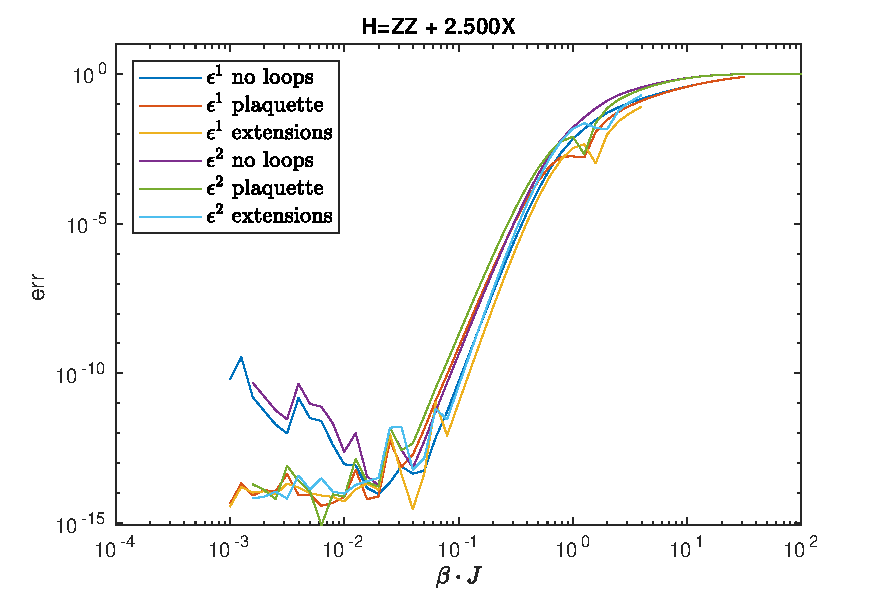
\includegraphics[width=\textwidth]{Figuren/benchmarking/2D_Err01_t_sing.pdf}
    \caption{The errors $\epsilon^i$ for 2D \Gls{TFI} model. }
    \label{fig:res2d:n1:tising}
\end{figure}

\subsubsection{Heisenberg}

The results for the harder to simulate Heisenberg model are shown in \cref{fig:res2d:n1:heis}. The conclusion is once again that the error $\epsilon^2 > \epsilon^1$ most of the time. The loops are absolutely a big improvement for  the results at low $\beta$. The loop extension also help to lower the error considerably.

\begin{figure}[!htbp]
    \center
    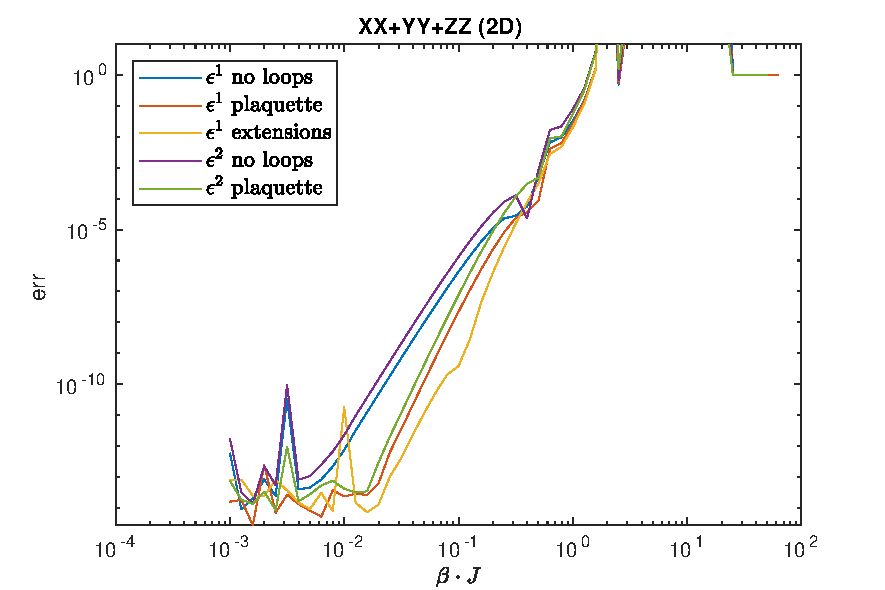
\includegraphics[width=\textwidth]{Figuren/benchmarking/2D_Err01_heis.pdf}
    \caption{The errors $\epsilon^i$ for 2D Heisenberg model. }
    \label{fig:res2d:n1:heis}
\end{figure}

\subsection{Conclusion}

It is interesting to compare the no loops errors from 2D with (\cref{fig:benchmark:tising} A:5) and (\cref{fig:benchmark:tHeisenberg} A:5), the equivalent 1D errors.  They roughly match up, as can be expected. A similar observation can be made for lower order constructions.

This places the additional improvement of the error due to single extensions into context: they make an improvement, but one can expect the higher order expansion with same bond dimension to be just as successful.

In general, the results above show that the cluster expansions are also promising in 2D setting. The fact that the version with plaquette extensions works well also opens up the pathway for simulations in higher dimension. The computation of the 'linear' blocks scale with the number of legs. The generalisation from 2x2 plaquette term to 2x2x2 cube should still be feasible, as the solvers are cable of handling systems with 8 sites.

\section{Phase diagram 2D Transverse Field Ising model} \label{subsec:2dpahsediag}

Now we have an idea how accurate the cluster expansions is, we can use it to calculate the thermodynamic properties of the transvere field Ising model. The sampling of points was explained in \cref{sec:phase_diag}.

As a reference, \cref{2dtisingphasediag} is shown once more

\begin{figure}[H]
    \center
    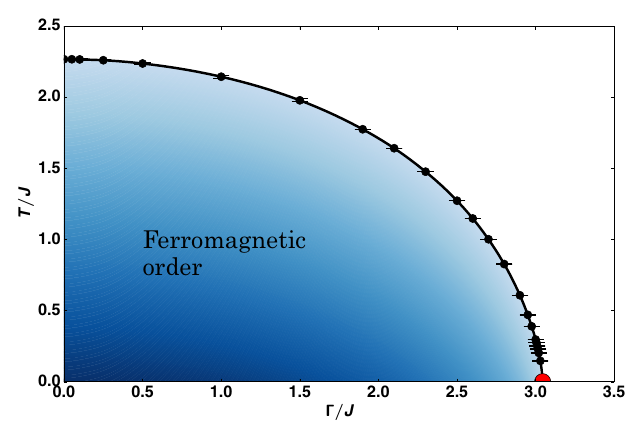
\includegraphics[width=\textwidth]{Figuren/phsyics/2disingphase.png}
    \caption{Phase diagram for 2D transversal Ising model. Figure taken from \cite{Hesselmann2016}}
    \label{2dtisingphasediag2}
\end{figure}

At the relevant temperature, an order 5 series expansion without loops is sufficient. This keeps the bond dimension small and hence the environment can be computed faster with VUMPS.

\subsection{Classical Ising phase transition}
The classical ising model on a square lattice has an exact solution. Onsager calculated the critical temperature to be $T_c = \frac{2 J}{k \ln(1+\sqrt{2}) } \approx 2.69185$. A test for the construction is to simulate this and compare the fitted (see \cref{subsec:qphasediag} ) results.

The results are shown in \cref{fig:phase:g0:full}. Each of the figures has 4 different subplots. Left upper corner shows m vs T. For low T, there is clearly a nonzero macroscopic magnetisation, while high T has a zero expectation value as expected. The other three plots show the data collapse of the finite size scaling of the entanglement entropy $S$, the correlation length $\xi$ and the magnetisation $m$. $\delta$ is marek gap, a measure for the system size as explained in \cref{subsec:fss}.

\begin{figure}
    \center
    \includegraphics[width=\textwidth]{Figuren/phasediag/g0/Full.pdf}
    \caption{  }
    \label{fig:phase:g0:full}
\end{figure}

\todo{new figure with entropy formula fixed 6S/c instead of cS/6}

Near criticality they collapse well, but away from the critical point there is quite some systematic variation. The reason is shown in \cref{fig:crit:qtran}. Only in some limited range around the critiacal region, the universal scaling holds.

A more zoomed in version is shown in \cref{fig:phase:g0:zoomed}. Clearly. the data collapses a lot better as expected.
\begin{figure}
    \center
    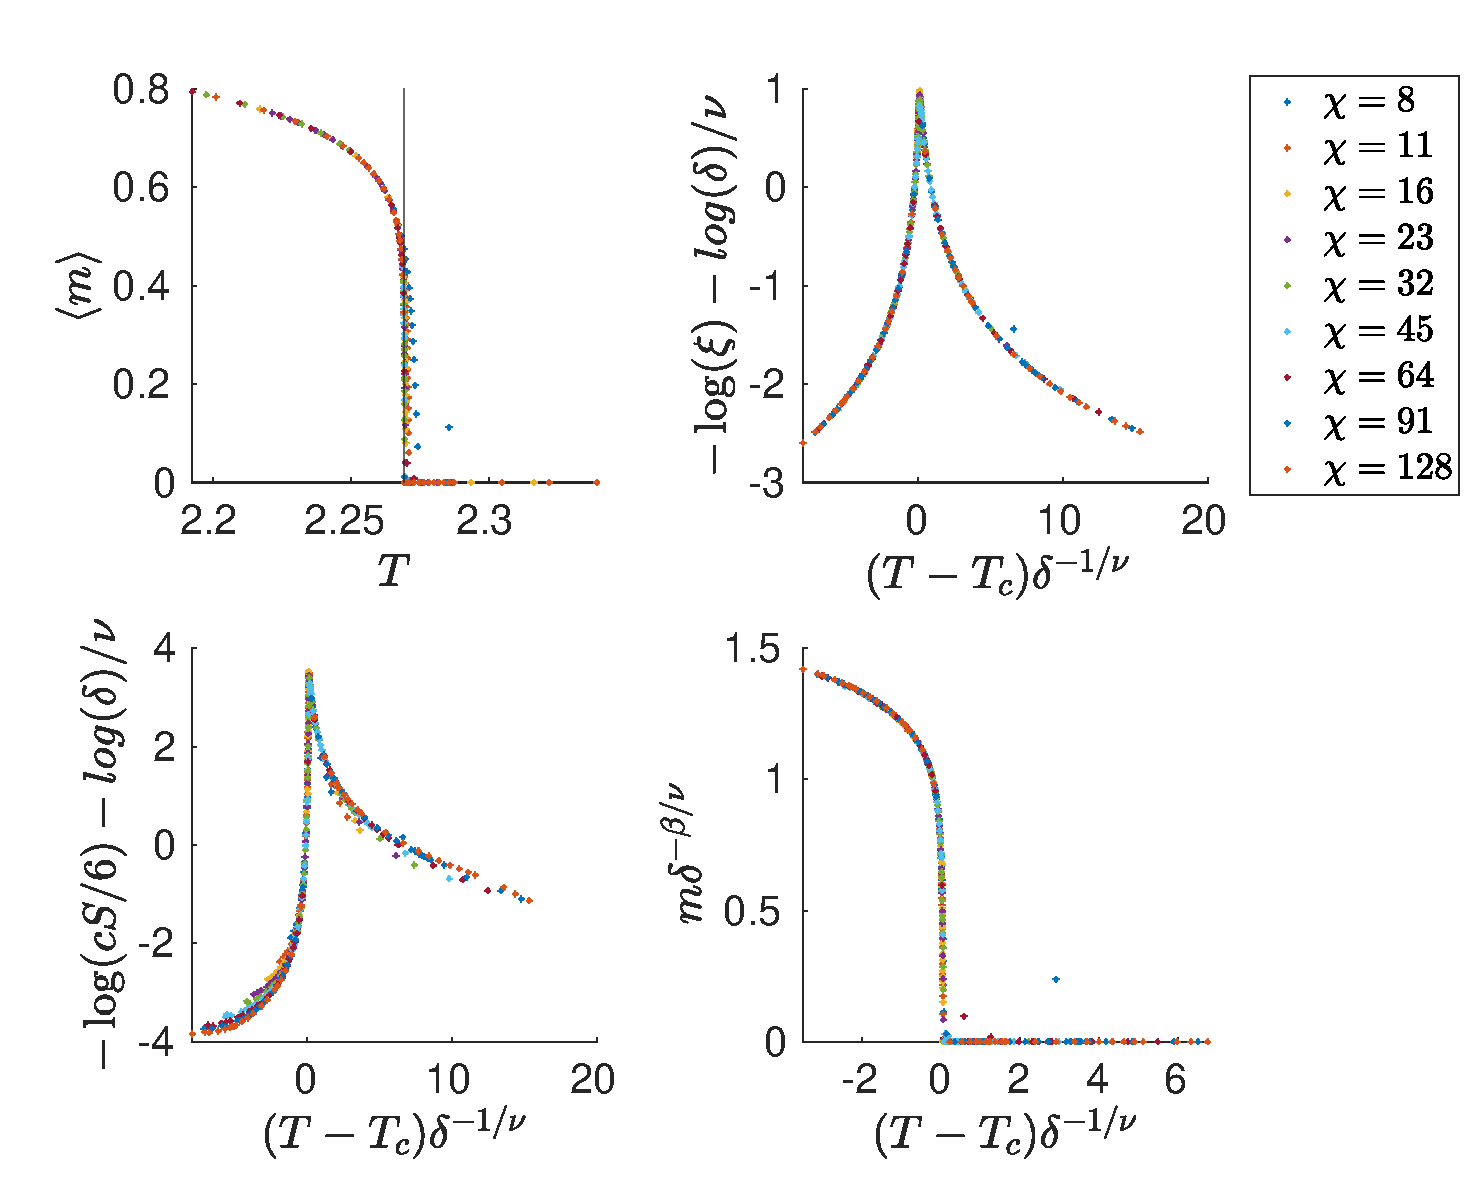
\includegraphics[width=\textwidth]{Figuren/phasediag/g0/zoomed.pdf}
    \caption{  }
    \label{fig:phase:g0:zoomed}
\end{figure}
In fact, the data collapses so well we could determine the the critical exponents and the temperature with the given data.

\todo{provide numbers for fit}

\subsection{g=2.5 phase transition }

The previous example simulated the classical 2D ising model. The question is whether this result will carry on into the quantum regime.The results for the full phase diagram \cref{fig:phase:g25:full} and or points in direct neighbourhood of the phase transition \cref{fig:phase:g25:zoomed} are similar to the 1D case.

Of course, quantitive details are different: the phase transition happens at $T\approx 1.274$ and the maximum magnetisation is lower than 1, in accordance to \cref{2dtisingphasediag}. The variation of m around the critical temperature for different bond dimensions is much higher. A much larger $\chi$ is needed for the fixed point MPS. This is not necessarily a problem, as this gives better data for the finite size scaling.

\begin{figure}
    \center
    \includegraphics[width=\textwidth]{Figuren/phasediag/g25/Full.pdf}
    \caption{  }
    \label{fig:phase:g25:full}
\end{figure}

\begin{figure}
    \center
    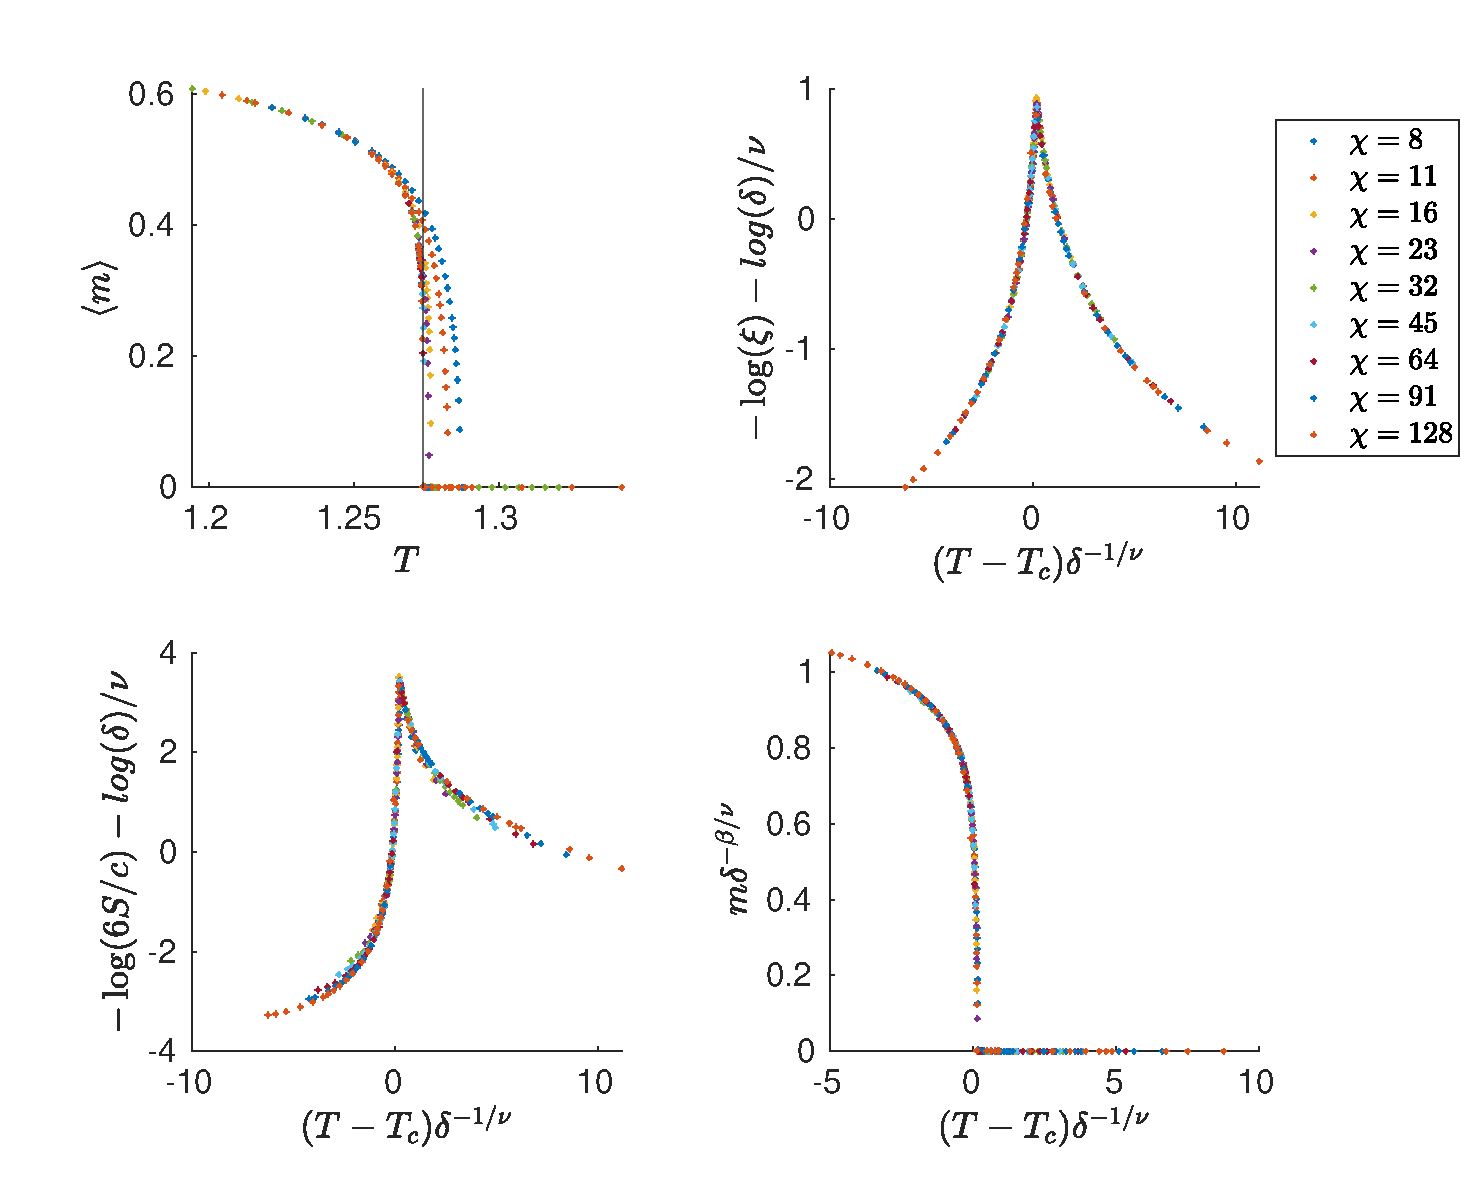
\includegraphics[width=\textwidth]{Figuren/phasediag/g25/zoomed.pdf}
    \caption{  }
    \label{fig:phase:g25:zoomed}
\end{figure}

There is no analytical expression for critical temperature known. With quantum monte carlo techniques, a value of $T_c=1.2737(6)$ is obtained, while state of the art tensor network techniques provide a value of $T_c=1.2737(2)$ \cite{Czarnik2019}

With the series expansion from this paper and Vumps, $T_c=1.2736(6)$, indicating that this faithfully captures the physics. To put his into context: the directly calculated error $\epsilon^{2}$  at $T=1.2$ was around $0.006$.

\subsection{T=0.7 quantum phase transition }\label{tphasetranssubsec}

Up until now, the phase diagram in \cref{2dtisingphasediag2} was explored at constant g in function of T, but of course there is also a transition at constant T and varying g.  T = 0.7 is chosen. The results are shown in \cref{fig:phase:t07:full}.

\begin{figure}
    \center
    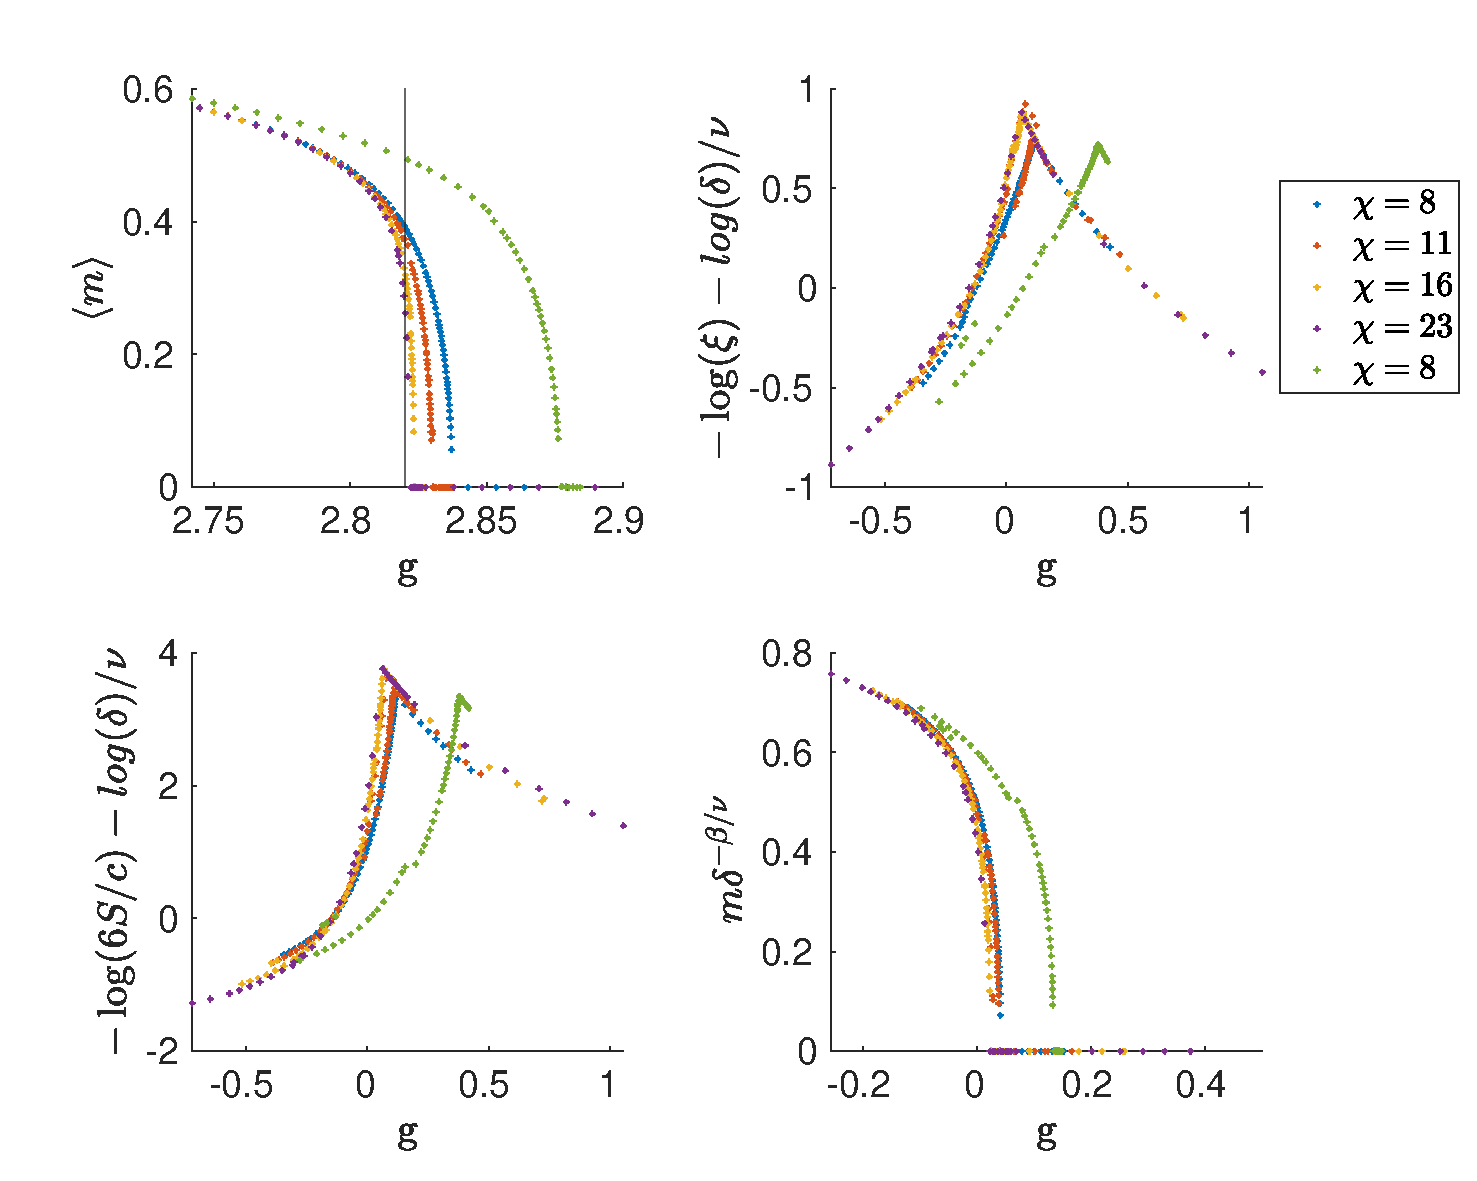
\includegraphics[width=\textwidth]{Figuren/phasediag/t07/full.pdf}
    \caption{Results for $T=0.7$ phase transition. The green points are a truncated order 6 construction, the others order 5.  }
    \label{fig:phase:t07:full}
\end{figure}

Clearly, the results do not collapse as well as for the other models. The reason is that the order of the expansion is not high enough. The green curve is order 6, where virtual level is truncated to dimension 20. The others are order 5. Both include loop contributions, as opposed to the previous results. The green and blue curve both have MPS bond dimension $\chi=8$, but predict quite different magnetisation for large g. This shows that for $g>0.7$, order 5 is not sufficient anymore.

\begin{figure}
    \center
    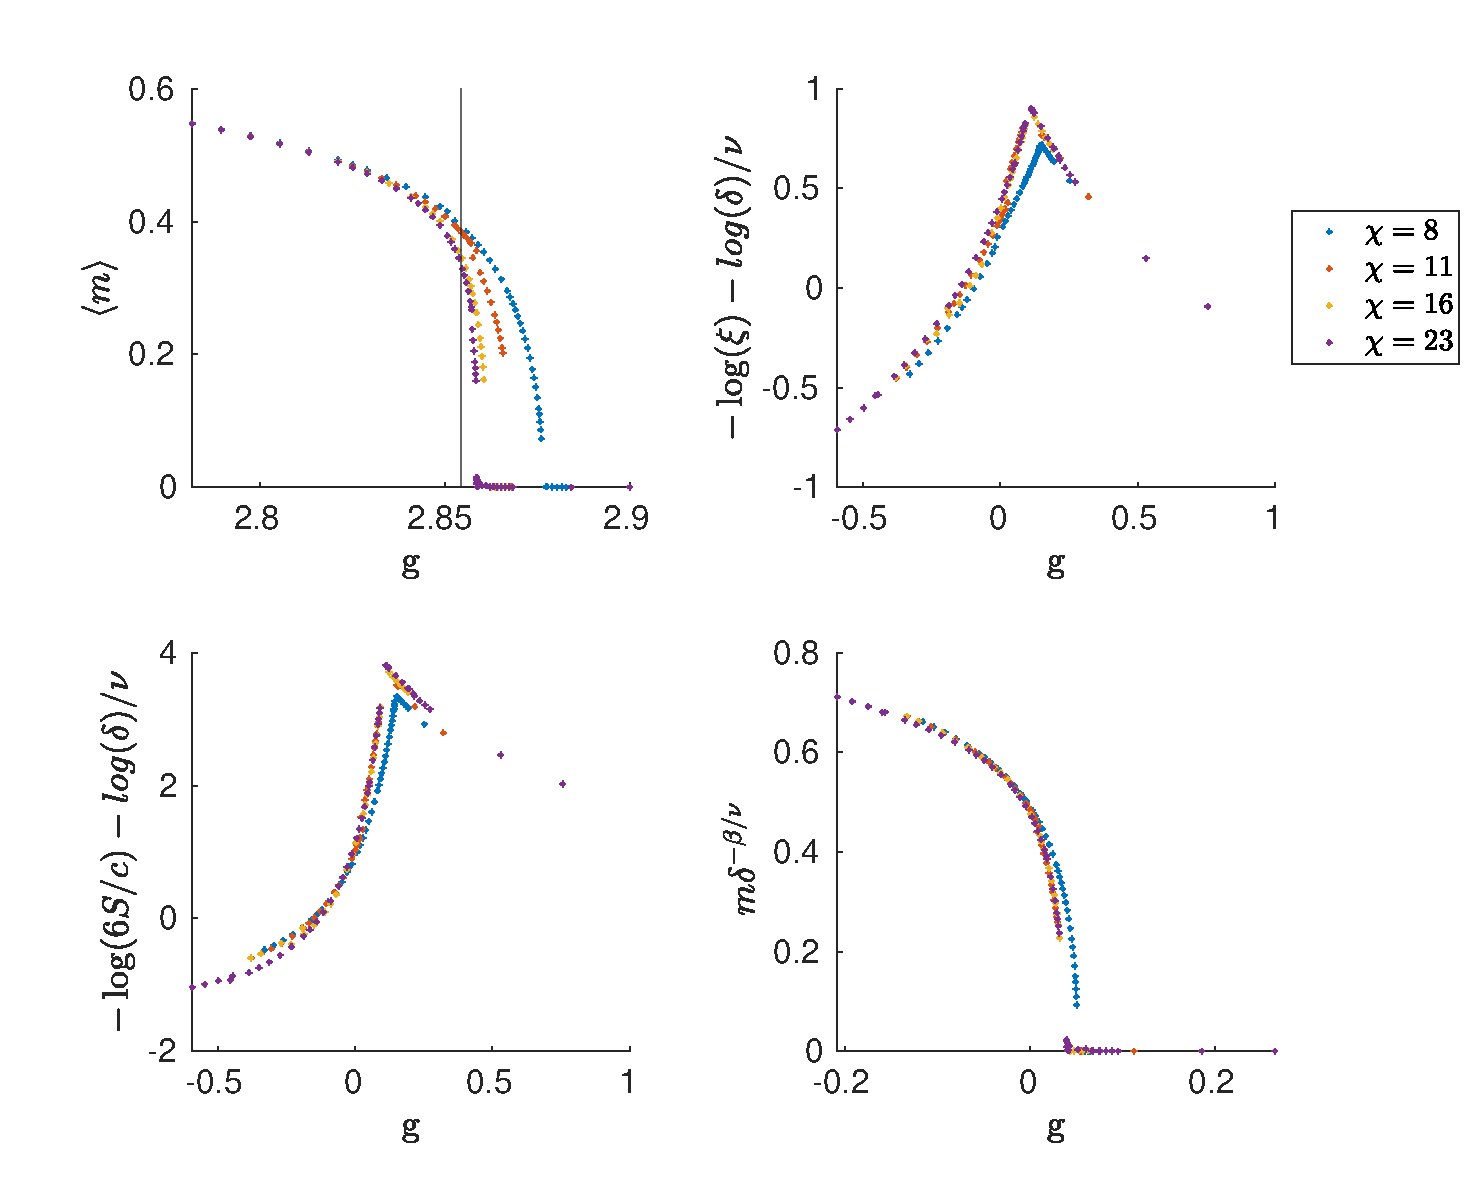
\includegraphics[width=\textwidth]{Figuren/phasediag/t07/zoomed2.pdf}
    \caption{Results for $T=0.7$ phase transition. The cluster expension is of order 6.}
    \label{fig:phase:t07:full2}
\end{figure}

A more accurate version is shown in \cref{fig:phase:t07:full2}. Here, all the cluster expansions are of order 6 with a total bond dimension of ($D = 1+4+16+20$) instead of ($D = 1+4+16$). The results, fitted without $\chi=8$ due to obvious finite size effects, show a much better collapse.

\subsection{Tricritical point}

Now that we know the critical transveral field can be determined, all the tools are present to extrapolate the tricritical point, indicated by a red dot in \cref{2dtisingphasediag2}. To achieve this, the following scaling relation can be used:
\begin{equation}
    T_c = \left| g_c-g_{c,q} \right|^{z \nu_{3D}}
\end{equation}
Near the critical point, the critical temperature $T_c$ and the critical transversal field $g_c$ are related to each other by the value of the quantum critical point $g_{c,q}$ and critical exponent $z=1$ and $\nu_{3D} \approx 0.62998$ \cite{Hesselmann2016}.

This could perfectly be done, given enough computation time to calculate for many temperatures the critical transversal field with a finite size scaling, similar to \cref{tphasetranssubsec}. Possibly, also a scaling in truncation dimension D for the cluster expansion is needed.

\subsection{Going beyond }
With all the built machinery to construct cluster expansions, is logical to calculate the phase diagram with increased precision.

\subsubsection{Higher order}

Going to higher order (i.e. longer linear chains) and adding the single loop contribution works well. The bond dimension of largest virtual level (3 in this case) can be truncated in the construction. The linear and non-linear solver find the least squares solution to the problems.

Care has to be taken in order to not violate one of the conclusions in 1D: never construct a longer chain than the previously fully solved one. For instance if the bond is truncated to 10, the linear chains can be constructed up till order 4. This means \cref{eq:cross_terms:order4} can be added but not \cref{eq:cross_terms:order5}, because the longest chains are order 5. Level 5 can still be constructed and contracted easily, but virtual level 3 has a bond dimension of 64. Compared to the previous bond dimensions (1,4 and 16) this is quite large and needs to be truncated.

\subsubsection{Loops and extensions}\label{subsec:results:loops_and_ext}
Adding loops decreases the error. but there is also a surprising result: all possible loop extensions result in a higher error. The fluctuation increases drastically. With increasing bond dimension $\chi$, this is somewhat better but still not good enough.
The question is wether this is a result of a failing cluster expansion, or inability VUMPS to calculate the correct environment. During my thesis, my focus has largely been on the first case. After all, the framework was completely build from scratch and errors happen, and there is no guarantee that the series even converges. But introduction of very strict variants, such as the generalization to type E, where left/upper extension have level a and the right/lower extensions are of type a':
\begin{equation}
    \vcenter{ \hbox{  \pepob{5}{3}{{
                        "-","-","-","-",
                        "-","a","$\alpha$","-",
                        "-","-","$\alpha$","-"}}{{
                        "-","-",
                        "-","-",
                        "-","$\alpha$",
                        "-","$\alpha$",
                        "-","-"}}{{
                        1,1,1,1,1,
                        1,0,0,0,1,
                        1,1,0,0,1}} }} \\
    \vcenter{ \hbox{  \pepob{5}{3}{{
                        "-","-","-","-",
                        "-","0","$\alpha$","-",
                        "-","-","$\alpha$","-"}}{{
                        "-","-",
                        "-","-",
                        "a'","$\alpha$",
                        "-","$\alpha$",
                        "-","-"}}{{
                        1,1,0,1,1,
                        1,1,0,0,1,
                        1,1,0,0,1}} }}
\end{equation}
Introduce these variations.

The VUMPS producedure come with 2 implicit assumptions: the original version was derived for hermitian hamiltonians. The MPO resulting from the traced PEPO  from the culster expansion is not an hermition MPO.

A second assumption made during this thesis is that the wave function can be represented by a 1by1 unit cell. Despite efforts made, the multisite version \cite{Nietner2020} doesn't seem to produce sensible results, even for version where 1by1 unit cell does give the right results.

It's clear that more research is needed here. One way to locate the problem would be to use another algorithm to contract the network, such as corner transfer matrix renormalization group (CTMRG) as used in  cite{Czarnik2019}, or even using the single site VUMPS algorithm combined with blocking:

\begin{equation}
    \vcenter{ \hbox{  \pepob{4}{4}{{
                        "","-","",
                        "","","",
                        "","","",
                        "","-","",}}{{
                        "","-","",
                        "","","",
                        "","","",
                        "","-","",}}{{
                        1,4,4,1,
                        4,0,0,4,
                        4,0,0,4,
                        1,4,4,1}} }} \cong  \vcenter{ \hbox{  \pepob{3}{3}{{
                        "","",
                        "","",
                        "","",}}{{
                        "","","",
                        "","","",}}{{
                        1,4,1,
                        4,0,4,
                        1,4,1}} }}
\end{equation}

\todo{complex matrices instead of real ones??}

\subsubsection{Better extrapolation}\label{sssec:better_Extrap}

The spirit behind finite size scaling is to calculate more with the data availalbe. In \cref{subsec:fss}, 2 additional varariations were suggested. One is to account for the subleading finite size corrections, the other to cange the way of calculating $\delta$.

\paragraph{Subleading corrections}
Intruducing subleading corrections requires 4 parameters for each fitted universal function: $\omega$,$\phi$,$c$ and $d$ from \cref{ea:subleadparam}. Compared to the one parameter $T_c$ or $g_c$, this is a lot and can be used to make many graphs collapse into a singlge graph. The analysis in \cite{Wang2006} curefully estimates the error made with the fitting procedure. A similar amount of rigour would be required to fully trust the results.

Nevertheless, fitting with subleading corrections results in critical temperatures close to the ones fitted without, and the subleading exponents are close to 1, as expected from the subleading series expansion.

\paragraph{ Choice  $\delta$  }

Different choices of $c_i$ in \cref{eq:cit_delta} are possible to construct $\delta$.  Variantional optimisation was doen as suggested in \cite{Nietner2020}. Both the x and y axis should be normalised, because depending on $\delta$ the scale changes. If scaled based on the outer points, there is a flaw in the fitting procedure.  The variational minimum goes to a point where at least for one point $\delta$ is extremely close to 0, and hence everything on the x axis except that point is pinched together, resulting in very small relative error. Therefore, it is better to normalise according to the points a e.g. 25th percentile and 75th percentile of the range on the  axis.

This improves the collapse, but is not clear how much the prediction of $T_c$ or $g_c$ is improved.

\subsection{Conclusion}

The conclusion from the direct results in \cref{sec:results2d} seems to carry over to a lattice in the thermodynamic limit very well. Comparison with the critical temperatures from literature confirmed that this method is able to approximate the operator $\exp(-\beta \hat{H})$ very well, even for a cluster expansion of order 5 without loops. This has only a bond dimension of 21, enabling the use of larger VUMPS bond dimension.

The path for determining a value for the tricritical, an important test for any method, is clear and mostly requires more precise data. With more data points, and carefull analysis of the end results, the techniques of \cref{sssec:better_Extrap} could be used to calculated even more precise results.



\section{Conclusion}
This chapter tested the proposed cluster expansion in a number of different ways. In \cref{sec:results1d}, the accuracy of the constructions introduced in \cref{H4_mpo_cons} were measured against the exact exponentiation of the Hamiltonian on a cyclic chain. It was shown that taking the pseudoinverse as explained in \cref{subsec:linear_solver} is absolutely necessary to obtain a converging cluster expansion.
A surprising result is that the strict types, which only add the explicitly calculated blocks to the expansion but not longer chains, result in a less performant cluster expansion. Independent of the Hamiltonian, type A results in the smallest errors and the smallest bond dimension. The largest virtual level can be truncated to any desired bond dimension. Constructing an explicit rotationally invariant \Gls{MPO} does not result in a lower error.
Overall, the 1D results show that an order 7 construction (bond dimension 86) can represent  $e^{\beta \hat{H}}$ up to machine precision for larger imaginary time steps. For the transverse Ising model, $\beta_{exact} = 0.6$ while for Heisenberg it amounts to $\beta_{exact} = 0.05$.
The construction from 1D was generalised to 2D in \cref{H4_pepo_cons}. \cref{sec:results2d} presented the 2D results in a manner very similar to the 1D results. It was found that the 1D construction generalises well to 2D. Beside the equivalent blocks from 1D, also the loop contribution are important to keep the error low. Higher extensions improve upon the result, but they also require a large bond dimension. The results are somewhat less reliable than the 1D counterpart, because even with reduced density matrices, it is hard to contract a \Gls{TN} large enough to capture all the details of the model.
The fact that linear blocks and only one single loop are able to capture the essence of the exponential opens up the possibility to generalise the method to 3D setting.
With the results from these sections, it is clear that this method holds some real potential. In \cref{subsec:2dpahsediag}, some phase transitions are calculated with the constructed tensor exponentials in combination with \Gls{VUMPS}. The $g=0$ and $g=2.5$ critical temperatures $T_c$ match very well with the values found in literature. Calculation of the $T=0.7$ phase transition shows that also closer to the quantum critical point, (quantum) critical behaviour is found. The path is open to calculate the tricritical point of the 2D \Gls{TFI} model with the current methods.

\chapter{Conclusion and Outlook}\label{Chap7}
\section{Conclusion}

In \cref{chap1} the quantum many-body problem was introduced as one of the challenges facing modern physics. The problem is not related to the theory, but to the practical difficulty of calculating and simulating the properties of strongly correlated matter. A macroscopic overview of one class of techniques, tensor networks, was given.
In \cref{chap2}, a brief introduction to tensor networks was given. The focus was mainly to provide some insight in the algorithm using the graphical tensor network notation. In particular, the VUMPS algorithm was explained. Also a technique was suggested to close the environment from below, because the current procedure only seems to work in specific cases \cref{subsec:results:loops_and_ext}.
\Cref{chap3} explains some concepts related to phases and phase transitions. The critical exponents associated with continuous phase transitions are discussed, together with a practical way called finite size scaling to obtain them from simulations. This sections also gives an overview of 2 important models in the field: the Heisenberg model and the Ising model in different dimension. Finally, the need for operator exponentials and tensor network methods to simulate time evolution are discussed.
\Cref{chap4} is the center point of this dissertation: it explains how the cluster expansions are made. This is written down in a very compact way, making abstraction of all implementation details and results.
\Cref{chap5} details the working of the 3 different solvers: a linear solver, a non-linear solver and a sequential linear solver. The linear solver must be implemented with great care in order to handle the ill conditioned inverses. This is done by calculating the pseudo-inverse instead of a full inverse. This can be done at the cost of an SVD decomposition per leg, while maintain the accuracy of inverting all the legs at once. Also, an algorithm for determining all possible virtual indices of a given map using PEPS contraction is given.  A starting point for exploring the source code is given.
\Cref{chap:results} finally quantifies the quality of the cluster expansions. This is done with respect to the exact solution in 1D and 2D. As second test, the thermal phase diagram of the transversal field Ising model is calculated. The numerical temperatures of the phase transition at constant transversal field correspond to the values in literature. A clear path is set out to calculate the quantum critical point.

\section{Outlook}

The cluster expansions have a lot of potential. In the course of one master dissertation, it is not possible to look into every possibility because a lot of groundwork need to be covered. Here are some interesting prospects: 

\paragraph{Real time evolution}

Some first test in 1D \cref{subsec_rt_evo} show that the method also works for real time evolution. \Cref{rt_tn_methods} introduced some methods to calculate time evolutions with tensor networks. Crucially, all these methods come with a detailed error analysis. For instance, some methods have a proven error per step of $O \left( \frac{t}{N}^2  \right)$ , resulting in an error of $O \left( \frac{t^2}{N}  \right)$ at time t. This can be made arbitrarily small.

\paragraph{Quantum critical point}

As stated in \cref{subsec:tricrit}, it should be possible to calculate the quantum critical point of the transverse Ising model using the current methods. This would allow to compare this method better with other methods in literature.

\paragraph{Lattices}

The whole thesis, a square lattice was used. This is definitely not the only choice. Other lattices could potentially result in even lower errors. Due to the generality of the solvers, this should be within reach given more time.

\paragraph{Higher dimensions}

A promising conclusion from \cref{subsec:2dpahsediag} is that a combination of linear blocks and simple loops seems sufficient to construct a good tensor network. This opens up the path to create a 3D version of the the operator $e^{\beta \hat{H}}$.  

\paragraph{Symmetries}

The boundaries of simulation could be pushed beyond what is possible in the current framework by incorporating all symmetries available (both spatial and internal). This already exists for diagonalisation (e.g. see \cite{Wietek2018}). Pushing the results.

\todo{reference}

\clearpage
\addcontentsline{toc}{chapter}{\protect\numberline{}{Bibliography}}

\bibliographystyle{elsarticle-num}
\bibliography{bib}

\cleartoleftpage

\end{document}
